%% abtex2-modelo-trabalho-academico.tex, v-1.7.1 laurocesar
%% Copyright 2012-2013 by abnTeX2 group at http://abntex2.googlecode.com/ 
%%
%% This work may be distributed and/or modified under the
%% conditions of the LaTeX Project Public License, either version 1.3
%% of this license or (at your option) any later version.
%% The latest version of this license is in
%%   http://www.latex-project.org/lppl.txt
%% and version 1.3 or later is part of all distributions of LaTeX
%% version 2005/12/01 or later.
%%
%% This work has the LPPL maintenance status `maintained'.
%% 
%% The Current Maintainer of this work is the abnTeX2 team, led
%% by Lauro César Araujo. Further information are available on 
%% http://abntex2.googlecode.com/
%%
%% This work consists of the files abntex2-modelo-trabalho-academico.tex,
%% abntex2-modelo-include-comandos and abntex2-modelo-references.bib
%%

% ------------------------------------------------------------------------
% ------------------------------------------------------------------------
% abnTeX2: Modelo de Trabalho Academico (tese de doutorado, dissertacao de
% mestrado e trabalhos monograficos em geral) em conformidade com 
% ABNT NBR 14724:2011: Informacao e documentacao - Trabalhos academicos -
% Apresentacao
% ------------------------------------------------------------------------
% ------------------------------------------------------------------------

\documentclass[
	% -- opções da classe memoir --
	12pt,				% tamanho da fonte
	openany,			% capítulos começam em pág ímpar (insere página vazia caso preciso)
	oneside,			% para impressão em verso e anverso. Oposto a oneside
	a4paper,			% tamanho do papel. 
	% -- opções da classe abntex2 --
	%chapter=TITLE,		% títulos de capítulos convertidos em letras maiúsculas
	%section=TITLE,		% títulos de seções convertidos em letras maiúsculas
	%subsection=TITLE,	% títulos de subseções convertidos em letras maiúsculas
	%subsubsection=TITLE,% títulos de subsubseções convertidos em letras maiúsculas
	% -- opções do pacote babel --
	english,			% idioma adicional para hifenização
	brazil,				% o último idioma é o principal do documento
	]{abntex2}

\let\newfloat\undefined
% ---
% PACOTES
% ---

% ---
% Pacotes fundamentais 
% ---
\usepackage{cmap}				% Mapear caracteres especiais no PDF
\usepackage{lmodern}			% Usa a fonte Latin Modern			
\usepackage[T1]{fontenc}		% Selecao de codigos de fonte.
\usepackage[utf8]{inputenc}		% Codificacao do documento (conversão automática dos acentos)
\usepackage{lastpage}			% Usado pela Ficha catalográfica
\usepackage{indentfirst}		% Indenta o primeiro parágrafo de cada seção.
\usepackage{color}				% Controle das cores
% \usepackage{graphicx}			% Inclusão de gráficos
\usepackage[pdftex]{graphicx}
\usepackage{subcaption}
\usepackage{afterpage}
\usepackage{listings}
\usepackage{rotating}
\usepackage{pdfpages}
%\usepackage{subfigure}
% \usepackage{geometry}
\usepackage{pdflscape}
% \usepackage{lscape}
% \usepackage[demo]{graphicx}
% \usepackage{caption}
% \usepackage{subcaption}
% \overfullrule=2cm
%comand para marcar overfull
%package to format capa e folha de rosto
\usepackage{ufmg}
\usepackage{float}
\setcounter{secnumdepth}{5}
% \usepackage{caption}
\usepackage[font=Large]{caption}
\usepackage{lipsum}
\usepackage{listings}

\renewcommand*{\cftdotsep}{1}
\setpnumwidth{3em}
\setrmarg{4em}

% \renewcommand\listfigurename{Lista de Figuras}
% \renewcommand\listtablename{Lista de Tabelas}
\addto\captionsbrazil{
%% ajusta nomes padroes do babel
\renewcommand{\bibname}{Refer\^encias}
\renewcommand{\indexname}{\’Indice}
\renewcommand{\listfigurename}{Lista de Figuras}
\renewcommand{\listtablename}{Lista de Tabelas}
\renewcommand\lstlistingname{Arquivo}
\renewcommand\lstlistlistingname{Lista de Anexos}
\renewcommand*{\lstlistingname}{Código}
%% ajusta nomes usados com a macro \autoref
\renewcommand{\pageautorefname}{p\’agina}
\renewcommand{\sectionautorefname}{se{\c c}\~ao}
\renewcommand{\subsectionautorefname}{subse{\c c}\~ao}
\renewcommand{\paragraphautorefname}{par\’agrafo}
\renewcommand{\subsubsectionautorefname}{subse{\c c}\~ao}
}

%for showing python code

\usepackage[scaled]{beramono}
\usepackage{minted}

% \usepackage{listings}
%  
% \lstset{
%   language=Python,
%   showstringspaces=false,
%   formfeed=\newpage,
%   tabsize=4,
%   commentstyle=\itshape,
%   basicstyle=\ttfamily,
%   morekeywords={models, lambda, forms}
% }
%  
% \newcommand{\code}[2]{
%   \hrulefill
%   \subsection*{#1}
%   \lstinputlisting{#2}
%   \vspace{2em}
% }

% ---
		
% ---
% Pacotes adicionais, usados apenas no âmbito do Modelo Canônico do abnteX2
% ---
% \usepackage{lipsum}				% para geração de dummy text
% ---

% \newcommand{\textbackslash}{\\}
% \newcommand{\textbackslash}{\\}
% \renewcommand{\textbackslash}{\}
% \providecommand{\&}{&}
% \providecommand{\bsl}{}%

% \renewcommand\contentsname{whatever}



% ---
% Pacotes de citações
% ---
\usepackage[brazilian,hyperpageref]{backref}	 % Paginas com as citações na bibl
%\usepackage[alf]{abntex2cite}	% Citações padrão ABNT
\usepackage[alf,abnt-url-package=url]{abntex2cite}

%\usepackage[alf,abnt-url-package=url]{abntex2cite}

% \usepackage[num]{abntex2cite}	% Citações padrão ABNT
% --- 
% CONFIGURAÇÕES DE PACOTES
% --- 
\providecommand{\textbackslash}{} 


% ---
% Configurações do pacote backref
% Usado sem a opção hyperpageref de backref
\renewcommand{\backrefpagesname}{Citado na(s) página(s):~}
% Texto padrão antes do número das páginas
\renewcommand{\backref}{}
% Define os textos da citação
\renewcommand*{\backrefalt}[4]{
	\ifcase #1 %
		Nenhuma citação no texto.%
	\or
		Citado na página #2.%
	\else
		Citado #1 vezes nas páginas #2.%
	\fi}%
% ---

\newcommand{\HRule}{\rule{\linewidth}{0.5mm}} % New command to make the lines in the title page

\graphicspath{{./Figures/}} % Specifies the directory where pictures are stored

% ---
% Informações de dados para CAPA e FOLHA DE ROSTO
% ---
\titulo{Mendel,MD: Desenvolvimento e validação de uma ferramenta online para análise de exomas humanos e investigação de doenças Mendelianas.}
\autor{Raony Guimarães Corrêa Do Carmo Lisbôa Cardenas}
\local{Belo Horizonte}
\data{2015}
\orientador{Prof. Dr. Sérgio Danilo Junho Pena}
\coorientador{}
\instituicao{%
  Universidade Federal de Minas Gerais - UFMG
  \par
  Instituto de Ciências Biológicas
  \par
  Programa de Pós-Graduação em Bioinformática}
\tipotrabalho{Tese (Doutorado)}
% O preambulo deve conter o tipo do trabalho, o objetivo, 
% o nome da instituição e a área de concentração 
\preambulo{Relatório final do projeto de tese apresentado ao colegiado do curso de Doutorado em Bioinformática como parte integrante dos requisitos para obtenção do título de Doutor em Bioinformática.}
% ---

% ---
% Configurações de aparência do PDF final

% alterando o aspecto da cor azul
\definecolor{blue}{RGB}{41,5,195}

% informações do PDF
\makeatletter
\hypersetup{
     	%pagebackref=true,
		pdftitle={\@title}, 
		pdfauthor={\@author},
		pdfsubject={\imprimirpreambulo},
		pdfcreator={LaTeX with abnTeX2},
		pdfkeywords={abnt}{latex}{abntex}{abntex2}{trabalho acadêmico}, 
		colorlinks=true,       		% false: boxed links; true: colored links
		linkcolor=blue,          	% color of internal links
		citecolor=blue,        		% color of links to bibliography
		filecolor=magenta,      		% color of file links
		urlcolor=blue,
		bookmarksdepth=4
}
\makeatother
% --- 

% --- 
% Espaçamentos entre linhas e parágrafos 
% --- 

% O tamanho do parágrafo é dado por:
\setlength{\parindent}{1.3cm}

% Controle do espaçamento entre um parágrafo e outro:
% \setlength{\parskip}{0.2cm}  % tente também \onelineskip \doublespacing
\DoubleSpacing
% ---
% compila o indice
% ---
\makeindex
% ---

% ----
% Início do documento
% ----
\begin{document}

\frontmatter
% Retira espaço extra obsoleto entre as frases.
\frenchspacing 

% %%%CAPA

\begin{center}
% image


\includegraphics[width=0.2\textwidth]{./Pictures/Logo_UFMG.jpg}


% 
\includegraphics[scale=0.1,keepaspectratio=true]{./Pictures/Logo_UFMG.jpg}
% Logo_UFMG.jpg: 860x336 pixel, 100dpi, 21.84x8.53 cm, bb=0 0 619 242

\textsc{\LARGE Universidade Federal de Minas Gerais}\\[1.5cm] % University name
\HRule \\[0.4cm] % Horizontal line
{\huge \textbf{Mendel,MD: Desenvolvimento e validação de uma ferramenta online para análise de exomas humanos e investigação de doenças Mendelianas.} }\\[0.4cm] % Thesis title
\HRule \\[1.5cm] % Horizontal line
\vspace{6em}

\begin{minipage}{0.4\textwidth}
\begin{flushleft} \large
\emph{Autor:}\\
\href{http://lattes.cnpq.br/0263349039132540}{Raony GCCL Cardenas} % Author name - remove the \href bracket to remove the link
\end{flushleft}
\end{minipage}
\begin{minipage}{0.4\textwidth}
\begin{flushright} \large
\emph{Orientador:} \\
\href{http://lattes.cnpq.br/5969241975196292}{Sérgio DJ Pena} % Supervisor name - remove the \href bracket to remove the link  
\end{flushright}
\end{minipage}\\[1cm]
 
\large \textit{Documento apresentado em cumprimento aos requisitos para obtenção do título de  Doutor em Bioinformática}\\[0.3cm] % University requirement text
\textit{no}\\[0.4cm]
Instituto de Ciências Biológicas\\[2cm] % Research group name and department name
{\large \today}\\[4cm] % Date
%\includegraphics{Logo} % University/department logo - uncomment to place it
\vfill
\clearpage % Start a new page


\end{center}

% ----------------------------------------------------------
% ELEMENTOS PRÉ-TEXTUAIS
% ----------------------------------------------------------
\pretextual

% ---
% Capa
% ---
\imprimircapa
% ---

% ---
% Inserir folha de aprovação
% ---

% Isto é um exemplo de Folha de aprovação, elemento obrigatório da NBR
% 14724/2011 (seção 4.2.1.3). Você pode utilizar este modelo até a aprovação
% do trabalho. Após isso, substitua todo o conteúdo deste arquivo por uma
% imagem da página assinada pela banca com o comando abaixo:
%
% \includepdf{folhadeaprovacao_final.pdf}
% %
% \begin{folhadeaprovacao}
% 
%   \begin{center}
%     {\ABNTEXchapterfont\large\imprimirautor}
% 
%     \vspace*{\fill}\vspace*{\fill}
%     {\ABNTEXchapterfont\bfseries\Large\imprimirtitulo}
%     \vspace*{\fill}
%     
%     \hspace{.45\textwidth}
%     \begin{minipage}{.5\textwidth}
%         \imprimirpreambulo
%     \end{minipage}%
%     \vspace*{\fill}
%    \end{center}
%     
%    Trabalho aprovado. \imprimirlocal, 24 de novembro de 2012:
% 
%    \assinatura{\textbf{\imprimirorientador} \\ Orientador} 
%    \assinatura{\textbf{Professor} \\ Convidado 1}
%    \assinatura{\textbf{Professor} \\ Convidado 2}
%    %\assinatura{\textbf{Professor} \\ Convidado 3}
%    %\assinatura{\textbf{Professor} \\ Convidado 4}
%       
%    \begin{center}
%     \vspace*{0.5cm}
%     {\large\imprimirlocal}
%     \par
%     {\large\imprimirdata}
%     \vspace*{1cm}
%   \end{center}
%   
% \end{folhadeaprovacao}
% % ---
% 
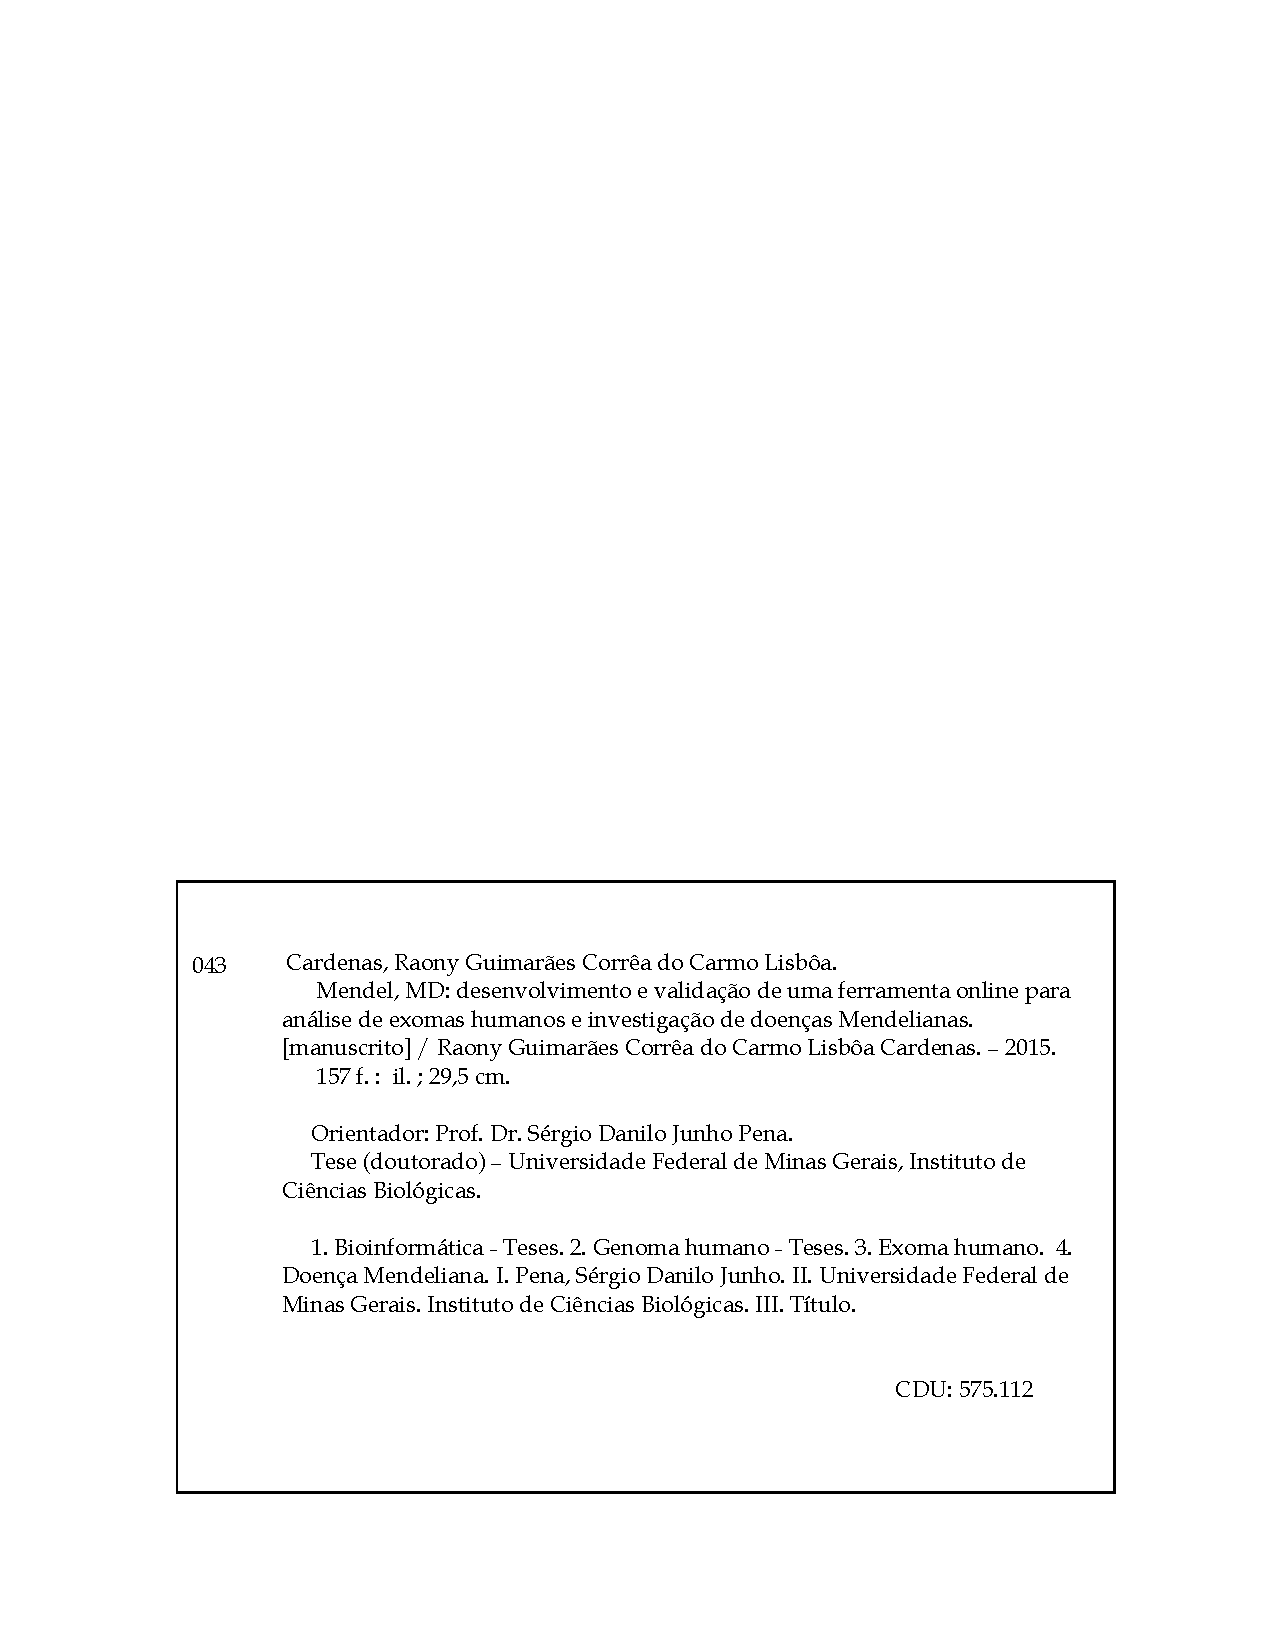
\includepdf{extras/ficha_catalografica.pdf}

\includepdf{extras/folha_de_aprovacao.pdf}

\pagenumbering{roman}

% % ---
% Dedicatória
% ---
\begin{dedicatoria}
 \vspace*{\fill}
 \centering
 \noindent
 \textit{Dedicado as minhas irmãs, Cecília, Duda e Isabel e ao meu irmão Pedro Henrique.} \vspace*{\fill}
\end{dedicatoria}
% % ---
% 
% % ---
% Agradecimentos
% ---


\begin{agradecimentos}

Gostaria antes de tudo de agradecer a minha família, em especial a minha querida avó Edna Guimarães Corrêa e a minha mãe Patrícia Do Carmo Lisboa Mouro que sempre fizeram de tudo para me dar a melhor educação possível.

A minha esposa Anna Kowalska Guimarães por todo amor e carinho que recebi e por sempre ter me apoiado muito quando decidi vir fazer meu Doutorado aqui em Belo Horizonte. Kocham Cię!

Ao Prof. Sérgio Danilo Junho Pena pela sua orientação e dedicação, por me ensinar os valores de um verdadeiro cientista e pelas valiosas lições que aprendi ao longo de meu Doutorado sob sua orientação.

Aos membros do Laboratório de Genômica Clínica Raquel Liboredo, Michele Pena, Tiago Magalhães, Lucas Santos, Natália Linhares, Maíra Freire e Fernanda Soardi e aos amigos do Laboratório de Genética e Bioquímica.

Aos pesquisadores Dr. Cascon Alberto, Dr. Christopher Carroll, Dr. Fowzan S. Alkuraya, Dr. Pia Ostergaard e Dr. Yaniv Erlich que contribuíram para este trabalho enviando seus exomas para serem analisados e validados pelo Mendel,MD. Sem essa contribuição esse trabalho não poderia ter sido realizado.

A pesquisadora Dra. Judith Conroy pela colaboração e as valiosas sugestões que foram feitas ao Mendel,MD.

Aos amigos do ICB em especial Thiago Mafra e Rondon Neto pelas valiosas discussões sobre Bioinformática que tivemos ao longo desse tempo.

Aos amigos do Hackerspace Área31 e Python User Group de Minas Gerais (PUG-MG) pela grande amizade e pelos encontros que tivemos nos bares de Belo Horizonte.

Aos meus amigos de infância Martielo Borelli e Miguel Rivero por terem me incentivado a estudar e a continuar aprendendo coisas novas.

Por último, mas não menos importante, gostaria de agradecer ao meu cachorro Einstein que sempre me acompanhou durante todo esse tempo nos passeios diários de reflexão e raciocínio.

\end{agradecimentos}
% % ---
% 
% % ---
% Epígrafe
% ---
% \begin{epigrafe}
%     \vspace*{\fill}
% 	\begin{flushright}
% 		\textit{``Meus estudos científicos têm me proporcionado grande satisfação \\
% 		e eu estou convencido que não demorará muito para que o mundo inteiro \\
% 		reconheça os resultados de meu trabalho. \\
% 		(Gregor Mendel)}		
% 	\end{flushright}
% \end{epigrafe}
%---

% ---
% RESUMOS
% ---
% addcontentsline{toc}{chapter}{Resumo}
% \section*{Resumo}
% \addcontentsline{toc}{section}{Resumo}

\addcontentsline{toc}{section}{Resumo}
% \section*{Resumo}

% resumo em português
\begin{resumo}

Com o advento dos métodos de sequenciamento de nova geração, o seqüenciamento de todo o exoma de um paciente tornou-se economicamente viável para realizar o diagnóstico clínico de doenças genéticas, incluindo as raras e complexas. 

A estratégia para a identificação de variantes patogénicas é complexa, uma vez que em todos os exomas existem entre 40-50.000 variantes em comparação com o genoma humano de referência. Para simplificar este procedimento, filtros computacionais são aplicados de forma sequencial com o objetivo de eliminar variantes comuns e sinônimas, reduzindo o tamanho da amostra total. 

Esse trabalho apresenta o desenvolvimento de uma ferramenta de Bioinformática chamada Mendel,MD, que é eficiente e sofisticada do ponto de vista computacional, e ao mesmo tempo, simples e amigável para ser utilizada por médicos e cientistas para auxiliar no diagnóstico de pacientes com doenças mendelianas.

A Análise de Filtros é um método que combina diferentes anotações, bases de dados e escores de patogenicidade, permitindo com isso reduzir o número de variantes e genes de cada caso clínico de milhares de candidatos para apenas algumas poucas dezenas.

Essa ferramenta foi validada com dados de 15 casos clínicos diferentes recebidos a partir de laboratórios especializados de diferentes países. Foi consistentemente possível identificar uma pequena lista de candidatos de genes causais, que incluiu o diagnóstico correto em todos os casos investigados.

Mendel, MD é uma ferramenta eficiente, segura e confiável na exploração de variantes de exomas de pacientes com Doenças Mendelianas, sofisticados do ponto de vista da bioinformática e ainda assim simples o suficiente para ser usado por médicos e cientistas para analisar rapidamente seus pŕoprios dados genômicos.

 \vspace{\onelineskip}
 \noindent
 \textbf{Palavras-chaves}: bioinformática, exoma humano, genoma humano, doença mendeliana, filtragem de variantes, anotação de variantes, análise de exomas, sequenciamento de nova geração.
\end{resumo}

% 
% resumo em inglês

\begin{resumo}[Abstract]
 \begin{otherlanguage*}{english}

With the emergence of next-generation methodology, the sequencing of the whole exome of a patient has become economically viable to perform the clinical diagnosis of genetic diseases, including rare and complex. 

The strategy for identification of pathogenic variants is complex, since in every exome there are between 40-50000 variants compared to the reference human genome. To simplify this procedure, computer filters are applied sequentially in order to remove common and synonymous variants, reducing the total sample size.

The study presents the development of a bioinformatics tool called Mendel,MD, which is efficient and sophisticated from the computational point of view, and at the same time, simple and friendly to be used by doctors and scientists to assist in the diagnosis of patients with Mendelian Disorders. 

The Filter analysis is a method that combines hundreds of different annotations, databases and pathogenicity scores, thereby allowing for reducing the number of gene and variants in each clinical case of thousands of candidates for only a few tens. 

This tool has been validated with data from 15 different clinical cases received from specialized laboratories in different countries. It was consistently able to identify a short list of candidates of causal genes, which included the correct diagnosis in all cases investigated.

Mendel, MD is an efficient, safe and reliable tool in the exploration of exome variants of patients with Mendelian disorders, sophisticated from the bioinformatics point of view and yet simple enough to be used by physicians and scientists to quickly analyze their own genomic data .

   \vspace{\onelineskip}
 
   \noindent 
   \textbf{Key-words}: exome sequencing, exome analysis, Mendelian disorder, next generation sequencing, variant calling, variant annotation.
 \end{otherlanguage*}
\end{resumo}


% 
% % resumo em francês 
% \begin{resumo}[Résumé]
%  \begin{otherlanguage*}{french}
%     Il s'agit d'un résumé en français.
%  
%    \vspace{\onelineskip}
%  
%    \noindent
%    \textbf{Mots-clés}: latex. abntex. publication de textes.
%  \end{otherlanguage*}
% \end{resumo}
% 
% % resumo em espanhol
% \begin{resumo}[Resumen]
%  \begin{otherlanguage*}{spanish}
%    Este es el resumen en español.
%   
%    \vspace{\onelineskip}
%  
%    \noindent
%    \textbf{Palabras clave}: latex. abntex. publicación de textos.
%  \end{otherlanguage*}
% \end{resumo}
% ---

% ---
% inserir lista de ilustrações
% ---
\phantomsection
\addcontentsline{toc}{section}{Lista de Figuras}
\pdfbookmark[0]{\listfigurename}{lof}
\listoffigures*
% \cleardoublepage
\clearpage
% ---

% ---
% inserir lista de tabelas
% ---

\phantomsection
\addcontentsline{toc}{section}{Lista de Tabelas}
\pdfbookmark[0]{\listtablename}{lot}
\listoftables*
% \cleardoublepage
\clearpage

%Inserir listings
%\addcontentsline{toc}{section}{Lista de Anexos}

% \phantomsection
% \addcontentsline{toc}{section}{\lstlistlistingname}
% \pdfbookmark[0]{\lstlistlistingname}{loa}

% \lstlistoflistings

% \clearpage
% \cleardoublepage

% ---

% ---
% inserir lista de abreviaturas e siglas
% ---

\phantomsection
\addcontentsline{toc}{section}{Lista de Abreviaturas e Siglas}
\begin{siglas}
  \item[AB3C] \textit{Associação Brasileira de Bioinformática e Biologia Computacional}
  \item[BFAST] \textit{Blat-like Fast Accurate Search}
  \item[BWA] \textit{Burrows-Wheeler Aligner}
  \item[CADD] \textit{Combined Annotation Dependent Depletion}
  \item[CENAPAD] Centro Nacional de Processamento de Alto Desempenho
  \item[CNV] \textit{Copy Number variations}
  \item[CSV] \textit{Comma Separated Values}
  \item[ESP] \textit{Exome Sequencing Project}
  \item[FSS] Síndrome de Freeman-Sheldon (\textit{Freeman-Sheldon Syndrome})
  \item[GATK] \textit{Genome Analisys ToolKit}
  \item[GL] \textit{Genome Library}
  \item[HGMD] \textit{Human Genome Mutation Database}
  \item[HGNC] \textit{HUGO Gene Nomenclature Committee}
  \item[HUGO] \textit{Human Genome Organisation}
  \item[INDEL] Inserção/Deleção (\textit{Insertion/Deletion})
  \item[LGC] Laboratório de Genômica Clínica
  \item[MVC] \textit{Model View Controller}
  \item[NCBI] \textit{National Center for Biotechnology Information}
  \item[NMD] \textit{Nonsense-mediated decay}
  \item[OMIM] \textit{Online Mendelian Inheritance in Man}
  \item[ORM] \textit{Object-relational mapping}
  \item[PB] Par de Base
  \item[SAM] \textit{Sequence Alignment/Map}
  \item[SBIS] \textit{Sociedade Brasileira de Informática em Saúde}
  \item[SGBD] Sistema Gerenciador de Banco de Dados
  \item[SIFT] \textit{Sort Intolerant From Tolerant}
  \item[SNP] Polimorfismo de Nucleotídeo Único (\textit{Single Nucleotide Polimorphism})
  \item[SQL] \textit{Structured Query Language}
  \item[SV] Variante Estrutural (\textit{Structural Variant})
  \item[TF] \textit{Transcription factor}
  \item[TFBS] \textit{Transcription Factor Binding Sites}
  \item[UTR] \textit{Untranslated Region}
  \item[VCF] \textit{Variant Call Format}
  \item[VEP] \textit{Variant Effect Predictor}
  
  
  
  
  
  
\end{siglas}
% % ---
% 
% \lhead{\emph{Abreviações}} % Set the left side page header to "Abbreviations"
% \listofsymbols{ll} % Include a list of Abbreviations (a table of two columns)
% {
% \textbf{SNP} & Single Nucleotide Polimorphism \\
% \textbf{Indel} & Insertion/Deletion \\
% \textbf{SV} & Structural Variantt \\
% \textbf{FSS} & Síndrome de Freeman-Sheldon \\
% \textbf{HGMD} & Human Genome Mutation Database \\
% \textbf{GATK} & Genome Analisys ToolKit \\
% \textbf{OMIM} & Online Mendelian Inheritance in Man \\
% 
% 
% \textbf{LAH} & \textbf{L}ist \textbf{A}bbreviations \textbf{H}ere \\
% \textbf{Acronym} & \textbf{W}hat (it) \textbf{S}tands \textbf{F}or \\
% }

% ---
% inserir lista de símbolos
% ---
% \begin{simbolos}
%   \item[$ \Gamma $] Letra grega Gama
%   \item[$ \Lambda $] Lambda
%   \item[$ \zeta $] Letra grega minúscula zeta
%   \item[$ \in $] Pertence
% \end{simbolos}
% ---

% ---
% inserir o sumario
% ---
\renewcommand\contentsname{Índice}

\pdfbookmark[0]{\contentsname}{toc}
\tableofcontents*
% \cleardoublepage
\clearpage
% ---

\mainmatter


% ----------------------------------------------------------
% ELEMENTOS TEXTUAIS
% ----------------------------------------------------------
%\textual




%start counting 1,2,3,4


% ----------------------------------------------------------
% Introdução
% ----------------------------------------------------------
% (1) Resumo, 
% (2) Introdução e Justificativa, 
% (3) Objetivos, 
% (4) Metodologia, 
% (5) Resultados preliminares, 
% (6) Cronograma das etapas a serem realizadas até o final do prazo de 48 meses de Doutorado e 
% (7) Bibliografia. 


\pagenumbering{arabic}

\chapter[Introdução e Justificativa]{Introdução e Justificativa}

Desde a invenção dos primeiros computadores em 1950, já existia uma certa discussão sobre o potencial de sua aplicação em áreas como a Medicina e a Biologia. Em 1968, A. A. Robertson  publicou um artigo com o título ``\textit{The use of computers in medicine with particular reference to general practice}'', porém, uma definição mais concreta sobre esta nova área da ciência que estava surgindo só começou a ser formulada em 1980 quando Edward Shortlife, Larry Fagan e Gio Wiederhold começaram a escrever o primeiro livro sobre Informática Médica para um curso de Medicina na Universidade de Stanford \cite{biomed_info}.

\section{Informática Biomédica}

De acordo com a terceira versão do livro ``\textit{Biomedical Informatics}'' publicada em 2006 por Shortlife, essa área de conhecimento corresponde ao estudo da informação biomédica, conectando dados e conhecimento, sendo responsável pelo armazenamento e recuperação dos dados, e da utilização de computadores para a solução de problemas médicos e auxílio na tomada de decisão.

Inicialmente esta área foi chamada de Informática Médica, sendo que o termo Informática Biomédica só começou a surgir a partir dos anos 90, com a expansão do Projeto Genoma Humano e da investigação e análise de dados aplicados em Biologia, através da conscientização de que os métodos e processos utilizados também poderiam ser aplicados na Biomedicina de uma maneira mais ampla e geral \cite{Kulikowski2012}.

Apesar de Informática Biomédica ser o termo mais adotado atualmente, ainda existe uma grande discussão sobre a real definição do seu significado e quais são as suas áreas de atuação. Um exemplo dessa discussão é o fato de que as associações representantes da área nos Estados Unidos ainda são chamadas de ``informática médica'' como a ``\textit{American Medical Informatics Association}'' e ``\textit{International Medical Informatics Association}''. No Brasil a associação representante desta área chama-se Sociedade Brasileira de Informática em Saúde (SBIS) \footnote{\url{http://www.sbis.org.br/}}, essa associação foi fundadada em 1986 pelo Prof. Renato Sabbatini com o objetivo de promover a troca de idéias e a apresentação de resultados nas área de Informática em Saúde, Telemedicina e Bioinformática.

De acordo com Bernstam \cite{Bernstam2010} em seu artigo ``\textit{What is Biomedical Informatics}'' publicado em 2010, a Informática Biomédica pode ser definida como a aplicação da Ciência da Informação e da Computação como dados e conhecimento para solução de problemas de interesse biomédicos.

\section{Bioinformática}

A Bioinformática é uma área multidisciplinar que integra os conhecimentos de diversas áreas diferentes como por exemplo: Biologia, Computação, Estatística, Matemática e Engenharia para realizar a análise de dados biológicos, além de construir ferramentas que permitam o armazenamento, organização, visualização e interpretação dos dados através do uso de um computador para realizar essas tarefas e gerar novo conhecimento.

A palavra Bioinformática foi utilizada pela primeira vez em um artigo publicado por Paulien Hogeweg em 1978 para descrever o estudo da informação em sistemas bióticos \cite{Hogeweg2011}. Desde então este termo se tornou mais abrangente, ganhando popularidade entre 1990 e 2000 no período chamado de revolução genômica quando passou a ser utilizado para representar a construção, manutenção e interpretação de grandes bancos de dados biológicos impulsionados pelo sucesso do Projeto Genoma Humano e o aumento da quantidade de dados biológicos disponíveis.

Apesar de Informática Biomédica e da Bioinformática serem áreas distintas, a pergunta que sempre surge neste ponto é qual seria então a interseção entre as duas áreas e esse assunto já foi amplamente discutido em estudos anteriores \cite{Practice2003, Martin-Sanchez2004}. De maneira geral podemos dizer que a Bioinformática possui um foco maior na Biologia Molecular enquanto a Informática Biomédica possui um foco maior na área Médica.

A associação que representa a área de Bioinformática no Brasil chama-se Associação Brasileira de Bioinformática e Biologia Computacional (AB3C) \footnote{\url{http://ab3c.cebio.org/}}.

\section{O Exoma}

Um éxon pode ser descrito como a parte do gene que fará parte do RNA maduro depois da remoção de todos os íntrons durante um processo de edição do RNA mensageiro que é chamado de \textit{RNA splicing}. A figura~\ref{fig:exon_image} apresenta o modelo de uma estrutura gênica com as suas regiões de íntrons, éxons e UTRs (\textit{Unstranslated Regions}) delimitadas com as cores vermelho, azul e cinza respectivamente.

\afterpage{
\begin{landscape}
\begin{figure}[p]
  \centering
    \Large\textbf{A estrutura de um Gene}\par\medskip
    \fbox{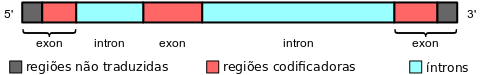
\includegraphics[width=1.4\textwidth]{../Figures/Gene_structure.png}}
    \caption[A estrutura de um Gene]{Esta figura mostra a estrutura simplificada de um gene com suas regiões de íntrons, éxons e UTRs (regiões não traduzidas). Fonte: \url{http://en.wikipedia.org/wiki/Exon}}
  \label{fig:exon_image} 
\end{figure}
\end{landscape}

\clearpage
}

Um exoma pode ser definido como a coleção de todos os éxons de um genoma. Essas  regiões correspondem a cerca de ~1.5\% do genoma humano (~30 Megabases) e estão divididas entre ~180,000 éxons. Apesar de constituir uma parte pequena do genoma, acredita-se que esta região contenha cerca de ~85\% das mutações associadas a doenças genéticas humanas \cite{Choi2009}. Isso demonstra a importância do estudo e da compreensão dessa região para ajudar na compreensão de doenças genéticas. Até fevereiro de 2015, 2937 genes associados a 4163 doenças mendelianas foram descobertos, porém cerca de 50\% das doenças mendelianas ainda não possuem um gene identificado. Portanto essa área ainda fornece grandes oportunidades para a descoberta de novos genes associados a doenças mendelianas \cite{Chong2015}. 


\section{Doenças Mendelianas}

Doenças Mendelianas são doenças genéticas que podem ser causadas por uma única mutação em um único gene. Além disso elas podem ser herdadas dos pais, ou seja, podem ser transmitidas de uma geração para outra de acordo com o modelo de herança proposto pelas leis de Mendel. Podemos citar como exemplos de doenças Mendelianas a anemia falciforme (OMIM:603903), a fibrose cística (OMIM:219700), a síndrome de Marfan (OMIM:154700) e a doença de Huntington (OMIM:143100). Existem atualmente mais de 4 mil doenças Mendelianas conhecidas de acordo com o site OMIM.

\section{Análise de Exomas para o diagnóstico de doenças Mendelianas}

Em 2008 \cite{Ng2008} publicaram um artigo contendo o sequenciamento do primeiro exoma humano (do pesquisador J. Craig Venter), mas apenas em 2009, foi publicado o primeiro artigo que utilizou o sequenciamento de exomas e o método de filtragem de variantes como uma prova de conceito para realizar a identificação do gene \textit{MYH3} (Gene ID: 4621) como sendo associado a Síndrome de Freeman-Sheldon (OMIM:193700) \cite{Ng2009}. Para identificar este gene foi necessário realizar o sequenciamento de 12 exomas, sendo 4 dos indivíduos afetados pela doença não relacionados e 8 indivíduos normais do projeto HapMap que foram utilizados como controles no processo de filtragem de variantes. Desde então centenas de outros estudos foram publicados com a utilização do sequenciamento de exomas de pacientes para descoberta de novas associações entre genes e doenças Mendelianas que até então ainda eram desconhecidas \cite{Bamshad2011a}.

A síndrome de Freeman-Sheldon (FSS) é uma doença genética causada por herança autossômica dominante, a forma mais conhecida pela literatura, e também por herança autossômica recessiva, ambas as formas são responsáveis por causar alterações ósseas e contraturas articulares levando a um fenótipo do paciente que é bastante característico.

A figura~\ref{fig:exome_filtering_example} mostra como foi o processo de filtragem de variantes que foi utilizado para a identificação do gene \textit{MYH3}. Podemos observar através desta figura que ao filtrar apenas por genes com mutações não sinônimas que estivessem presentes nos quatro indivíduos foi possível reduzir o número de genes candidatos para 2479 genes, ao eliminarem as mutações que estavam presentes apenas na última versão do dbSNP conseguiram diminuir a lista de genes candidatos para 53, ao utilizarem os dados dos 8 exomas controles do projeto HapMap conseguiram reduzir a lista de genes para 21, e por fim ao removerem os dados do dbSNP e do HapMap ao mesmo tempo, conseguiram reduzir a lista de genes candidatos para apenas 1 único gene. É importante notar que este gene também poderia ter sido encontrado utilizando outros critérios de filtragem como por exemplo o escore de SIFT e Polyphen-2 de cada variante. Este estudo mostrou que com a utilização de apenas 4 indivíduos não relacionados seria possível identificar o gene causador da doença Mendeliana investigada.

\afterpage{
\begin{landscape}
\begin{figure}[p]
  \centering
    \Large\textbf{Processo de Filtragem de Variantes para identificação de uma doença Mendeliana}\par\medskip
    \fbox{\includegraphics[width=1.4\textwidth]{../Figures/fss_filtering_process.png}}
    \caption[Processo de Filtragem de Variantes para identificação de uma doença Mendeliana]{Nesta imagem podemos verificar todas as etapas de filtragem que foram utilizadas para identificação do gene \textit{MYH3} como causador da síndrome de Freeman-Sheldon. Fonte: \cite{Ng2009}}
    
  \label{fig:exome_filtering_example}
\end{figure}
\end{landscape}

\clearpage
}

O gene \textit{MYH3} já era conhecido como sendo o causador síndrome de Freeman-Sheldon porém o estudo serviu como uma prova de conceito de que a tecnologia e o método poderiam ser utilizados para investigação de outras doenças onde o gene responsável ainda fosse desconhecido.

Ainda em 2009, Ng e o seu grupo \cite{Ng2010} descobriram a associação de um novo gene chamado \textit{DHODH} (Gene ID: 1723) como sendo o causador da Síndrome de Miller (OMIM\%263750) utilizando o mesmo método que havia sido validado pelo estudo anterior. Esta foi a primeira vez que a análise de exomas foi utilizada para identificação de um novo gene responsável por causar uma doença Mendeliana onde até então sua causa ainda era desconhecida.

Um estudo publicado em Fevereiro de 2015 \cite{Hu2015} realizou o sequenciamento do cromossomo X de 405 famílias com casos clínicos que ainda não haviam sido solucionados por outros métodos, e como resultado deste estudo, eles conseguiram identificar 7 novos genes associados a deficiência intelectual.

A figura~\ref{fig:exome_pubmed} mostra o crescimento do número de artigos publicados com a palavra ``\textit{exome}'' em títulos ou abstracts desde o ano de 2008 de acordo com o site Pubmed. 

Podemos observar que a partir de 2008 este número tem crescido a cada ano e que a previsão do número de artigos publicados em 2015 será ainda maior do que foi em 2014.

\afterpage{
\begin{landscape}

\begin{figure}[p]
    \centering
    \Large\textbf{Crescimento do número de artigos publicados com a palavra exome no Pubmed}\par\medskip
    \fbox{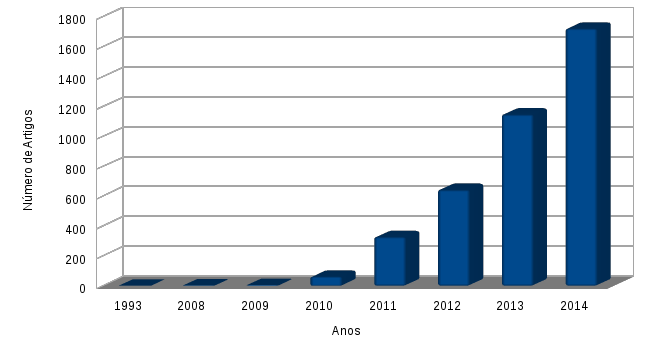
\includegraphics[width=1.5\textwidth]{../Figures/exome_pubmed.png}}
    \caption[Crescimento do número de artigos publicados com a palavra exome no Pubmed]{Nesta imagem podemos verificar o crescimento do número de artigos publicados com a palavra ``exome'' de acordo com o Pubmed ao longo dos últimos anos.}
    
  \label{fig:exome_pubmed}
\end{figure}
\end{landscape}

\clearpage
}

Esta técnica vem crescendo e se expandindo ao longo dos últimos anos e ainda deverá ser muito utilizada para realizar a investigação e o diagnóstico de doenças genéticas humanas. Apesar do sucesso comprovado deste método, ainda existem grandes desafios para que esta técnica seja completamente adotada e integrada dentro da prática clínica.

Atualmente existem poucas ferramentas desenvolvidas com o objetivo de auxiliar médicos e pesquisadores a analisarem este tipo de dado, e grande parte das ferramentas que existem, ainda exigem a execução de scripts e comandos manuais geralmente em um terminal Linux com o uso de parâmetros que possibilitem a exploração dos dados e a filtragem de variantes. A ausência de uma interface simples e amigável dificulta o acesso aos métodos e as informações por pessoas que não possuem conhecimentos sobre programação ou computadores.

Para este método atingir sua plenitude é preciso que existam programas práticos e acessíveis, que possibilitem a exploração dos dados não apenas por cientistas, mas também por médicos o outros profissionais da área da Saúde. 

É neste sentido que este trabalho foi iniciado, para ajudar traduzir os resultados obtidos a partir do sequenciamento de exomas e para tentar extrair informação útil deste tipo de dado para auxiliar no diagnóstico clínico de doenças Mendelianas.

\section{SNPs e Indels}

O Polimorfismo de Nucleotídeo Único (SNP) é uma variação genética causada pela alteração em um único par de base em uma posição específica do DNA.

A figura~\ref{fig:snp} mostra a representação gráfica de uma SNP e nela podemos observar a alteração de uma posição contendo GC para AT.

Os SNPs presentes nas regiões exônicas podem ser classificadas como sinônimas, ou seja, aquelas que não causam alteração na sequência de aminoácidos da proteína, e não-sinônimas, que são aquelas que causam alteração na sequência de aminoácidos da proteína. As mutações não-sinônimas podem ser classificadas como \textit{missense} e \textit{nonsense}. As mutações \textit{missense} são aquelas que causam uma substituição de um aminoácido por outro, e as mutações \textit{nonsense} são aquelas que causam a substituição de um aminoácido por um \textit{stop} códon, o que pode causar a produção de uma proteína não funcional.

\afterpage{
\begin{landscape}
\begin{figure}[p]
    \centering
    \Large\textbf{Representação gráfica de uma SNP}\par\medskip
    \fbox{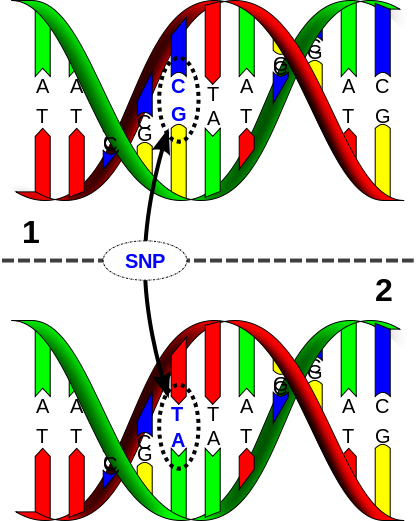
\includegraphics[width=0.6\textwidth]{../Figures/Dna-SNP.png}}
    \caption[Representação gráfica de uma SNP]{Representação gráfica de uma SNP mostrando uma alteração de G->C para A->T. Fonte: \url{http://en.wikipedia.org/wiki/Single-nucleotide_polymorphism}}
  \label{fig:snp}  
\end{figure}
\end{landscape}

\clearpage
}

Indel é um polimorfismo que corresponde a adição ou remoção de uma pequena sequência de bases de DNA, sendo que a maioria ocorre em regiões de repetição em tandem.

Na figura~\ref{fig:indel} é apresentado a representação gráfica de uma indel. Podemos observar uma deleção de duas bases AC na parte de cima e da inserção de duas bases AC na parte de baixo. Existem muitas indels associadas a doenças humanos e este é um assunto já bastante discutido em estudos anteriores \cite{Taylor2004, Haraksingh2013}.

\afterpage{
\begin{landscape}

 \begin{figure}[p]
   \centering
      \Large\textbf{Representação gráfica de uma Indel}\par\medskip
      
      \fbox{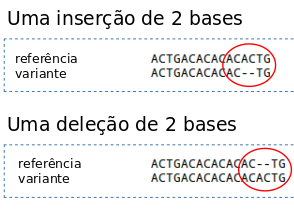
\includegraphics[width=1\textwidth]{../Figures/indel.png}}
      
      \caption[Representação gráfica de uma Indel]{Podemos observar uma deleção de duas bases AC na parte de cima e da inserção de duas bases AC na parte de baixo. Fonte: \url{http://genome.sph.umich.edu/wiki/Indel}}
      
     \label{fig:indel}
 \end{figure}
\end{landscape}

\clearpage
}


\section{Projeto Genoma Humano}

O Projeto Genoma Humano \cite{Lander2001} foi um consórcio científico internacional coordenado pelo \textit{National Institutes of Health} (NIH) com o objetivo de mapear todos os genes humanos e realizar o sequenciamento dos 3 bilhões de nucleotídeos do genoma humano.  Esse projeto teve um custo aproximado de 3 bilhões de dólares e em 2001, 10 anos após o seu início do projeto, foi publicado o primeiro rascunho do genoma humano.

Em 1998 o pesquisador J. Craig Venter deu início a um projeto paralelo em sua empresa \textit{Celera Genomics} para sequenciar o genoma humano usando uma técnica conhecida por \textit{Shotgun Sequencing} \cite{Venter2001}. Esta técnica permitiu o sequenciamento do genoma humano através da quebra do DNA em pequenos fragmentos de tamanho entre 100 e 1000 pares de base de maneira que a montagem do genoma pudesse ser realizada através do uso de programas de computador. Para isso foi necessário atingir uma cobertura mínima de 12X, ou seja, cada base do genoma foi sequenciada pelo menos 12 vezes para que essa montagem fosse possível.

Ambos os projetos foram publicados em 2001 pelas revistas \textit{Nature} e \textit{Science} \cite{Lander2001, Venter2001}.


\section{Projeto 1000 Genomas}

O ``\textit{1000 Genomes Project}'' \cite{Abecasis2010, Abecasis2012} é um projeto de colaboração internacional criado em 2009 com o objetivo de produzir um catálogo abrangente sobre as variações genéticas humanas. Até o momento já foram sequenciados e genotipados 2504 indivíduos\footnote{\url{http://www.1000genomes.org/data}}, esses dados estão disponibilizados de forma totalmente pública na internet para qualquer pesquisador que tiver interesse em realizar o download para analisá-los. Isso passou a permitir o uso desses dados de forma a auxiliar a clínica médica para realizar análises de exomas de pacientes e por exemplo para fazer a comparação de grupos de indivíduos normais presentes nesses bancos de dados com pacientes clínicos permitindo a eliminação de variantes controles que estivessem presentes no grupo de indivíduos de uma população.

Na tabela~\ref{1000genomes_ancestry} apresentamos informações sobre o número dos indivíduos que foram sequenciados e os grupos de ancestralidade que foram definidos pelos pesquisadores do projeto \textit{1000 Genomes}.

Site: \url{http://www.1000genomes.org}

\afterpage{
\begin{landscape}
\begin{table}[p]
\centering
\caption[Informações sobre a ancestralidade dos indivíduos que foram sequenciados pelo projeto \textit{1000 Genomes}]{Informações sobre a ancestralidade dos indivíduos que foram sequenciados pelo projeto \textit{1000 Genomes}.
Fonte: \url{http://www.1000genomes.org/about} }
\scalebox{1.5}{
\begin{tabular}{|l|l|}
\hline
\textbf{Populações}                       & \textbf{Número final de amostras} \\ \hline
\textbf{Ancestralidade Leste-Asiática}  & 504                           \\ \hline
\textbf{Ancestralidade Sul-Asiática} & 489                           \\ \hline
\textbf{Ancestralidade Africana}     & 661                           \\ \hline
\textbf{Ancestralidade Européria}    & 503                           \\ \hline
\textbf{Ancestralidade Ameríndia}    & 347                           \\ \hline
\textbf{Total}                            & \textbf{2504}                \\ \hline
\end{tabular}
}
\label{1000genomes_ancestry}
\end{table}
\end{landscape}

\clearpage
}


\afterpage{
\begin{landscape}

\begin{figure}[p]
  \centering
    \Large\textbf{Medicina Personalizada}\par\medskip
    \fbox{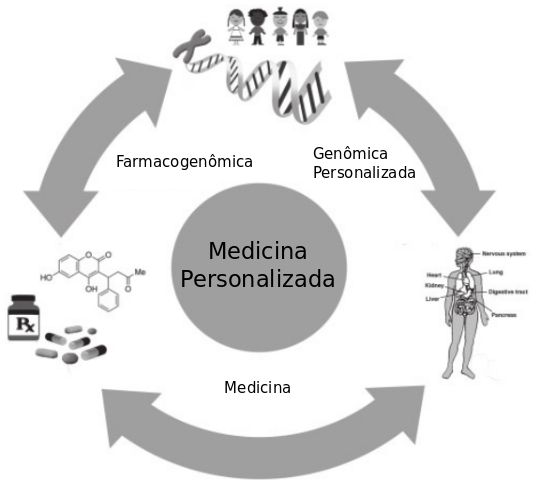
\includegraphics[width=0.9\textwidth]{../Figures/Personalized_medicine.png}}
    \caption[Medicina Personalizada]{Aqui podemos verificar que Medicina Personalizada é um termo que relaciona a Medicina Tradicional, a Genômica Personalizada e a Farmacogenômica. Fonte: \cite{Fernald2011a}}
  \label{fig:personalized_medicine}  
\end{figure}
\end{landscape}

\clearpage
}

\section{Projeto de Sequenciamento do Exoma}

O \textit{Exome Sequencing Project} (ESP) \cite{Fu2013} realizou até o momento o sequenciamento de 6515 exomas e embora os genótipos dos indivíduos não estejam disponíveis para download, é possível obter informações sobre a frequência das variantes que foram encontradas e este valor pode ser utilizado no processo de filtragem de variantes de indivíduos que possuam uma Doença Mendeliana específica.

Site: \url{http://evs.gs.washington.edu/EVS}

\section{Medicina Personalizada / Medicina de Precisão}

O termo ``Medicina Personalizada'' começou a surgir a partir de 1999 quando Robert Langreth e Michael Waldholz publicaram no jornal ``\textit{The Oncologist}'' o primeiro artigo com uma definição mais próxima da que temos atualmente sobre essa nova área da medicina \cite{Langreth1999}. A Medicina Personalizada é um modelo de saúde que propõe a realização de práticas utilizando dados como o perfil genômico do paciente para a tomada de decisão médica, com o objetivo de direcionar o melhor tratamento específico para cada paciente de acordo essas informações.

Na figura~\ref{fig:personalized_medicine} apresentamos uma imagem com a relação entre a Medicina Tradicional, a Genômica Personalizada e a Farmacogenômica. Essa área atualmente tem sido chamada de Medicina de Precisão \cite{Collins2015, Jameson} por ser um termo que representa melhor a aplicação dos dados genômicos de uma forma direcionada para atender as necessidades clínicas de cada paciente.


%Introdução
\chapter[Objetivos]{Objetivos}

\section{Objetivo Geral}

Estudar e desenvolver métodos e ferramentas que permitam o armazenamento e a análise de dados genômicos humanos possibilitando a investigação e o diagnóstico de casos clínicos de pacientes estudados pelo laboratório de uma maneira rápida e eficiente por médicos, cientistas e outros profissionais da área da Saúde. A seguir, apresentamos os objetivos específicos que foram definidos para serem realizados durante o desenvolvimento deste trabalho.

\section{Objetivos Específicos}

\begin{itemize}
  \item Desenvolver uma ferramenta que permita a médicos e cientistas investigarem os dados genômicos de seus pacientes.
  \item Gerar métricas de qualidade sobre o sequenciamento, a genotipagem e a cobertura do sequenciamento para cada indivíduo inserido no sistema.
  \item Desenvolver um \textit{pipeline} de anotação de variantes utilizando diferentes métodos e programas que ajudem na identificação de mutações que possam ser responsáveis por causar uma doença Mendeliana.
  \item Permitir a identificação de mutações em genes e doenças que já tiverem sido descritas pela literatura e de novas mutações e genes candidatos possivelmente associados com síndromes Mendelianas ainda não descritas pela literatura.
  \item Validar o programa desenvolvido com dados reais de pacientes do Laboratório de Genômica Clínica da Faculdade de Medicina da UFMG e com dados de exomas clínicos descritos anteriormente pela literatura.
  \item Estudar algoritmos de priorização de variantes como SIFT, Polyphen-2, CADD e Mutation Taster para estimar formas mais racionais de utilizar seus parâmetros para melhorar a análise dos dados.
\end{itemize}
%Objetivos
\chapter[Materiais e Métodos]{Materiais e Métodos}

\section{Hardware}

O desenvolvimento e as análises deste trabalho foram realizados em um computador Desktop com 500GB de espaço em disco, 4GB de RAM e 2 processadores Intel Pentium(R) Dual-Core E5400 @ 2.70GHz. Para o ambiente de produção foi utilizado um servidor Dell PowerEdge T-710 com 12TB de espaço em disco, 115GB de RAM e 24 cores Intel(R) Xeon(R) CPU X5660 @ 2.80GHz.

O pipeline de análise de exomas desenvolvido por este trabalho foi executado tanto no servidor local quanto no supercomputador do Centro Nacional de Processamento de Alto Desempenho de Minas Gerais (CENAPAD-MG) que possui 107 nós de computadores interligados através de uma rede rápida Infiniband com 8GB de RAM e 8 núcleos (Intel(R) Xeon(R) E5335 @ 2.00GHz) por máquina, totalizando 856 núcleos e 856GB de RAM disponíveis para serem utilizados para a execução de processos.

\section{Sistema Operacional}

O sistema operacional escolhido para o desenvolvimento deste projeto foi o Biolinux \cite{Field2006} atualmente na versão 8.0. Este é um sistema baseado em Ubuntu que foi criado e mantido pelo ``NERC Environmental Bioinformatics Centre'' na Inglaterra desde 2002, e foi escolhido por possuir mais de 500 pacotes pré-instalados para a Bioinformática, todos configurados e prontos para serem utilizados como por exemplo: Galaxy, Biopython, Bioperl, Bioconductor entre muitos outros pacotes que estão disponíveis no repositório criado pelo projeto que podem ser acessados no link abaixo.

\noindent
Site: \url{http://nebc.nerc.ac.uk/tools/bio-linux/}

\section{Linguagens e Frameworks Utilizados}

\subsection{Bash}

Bash é um ambiente ``\textit{shell}'' de programação unix que oferece uma linha de comando interativa e permite a execução de scripts e comandos que são executados de uma maneira sequencial com o objetivo de automatizar o uso de programas utilizados para realizar a análise dos dados genômicos. Diversos scripts em Bash foram desenvolvidos ao longo deste trabalho, inclusive para executar o pipeline de análise de exomas desenvolvido por este trabalho no supercomputador do CENAPAD-MG da UFMG.

\subsection{Python}

O Python é uma linguagem de programação orientada a objetos que foi criada por Guido Van Rossum em 1991 \cite{python}. Suas principais características são simplicidade, flexibilidade e elegância.

Todos os scripts deste projeto foram desenvolvidos utilizando Python 2.7 e atualmente estão sendo convertidos para Python 3. Esta linguagem foi escolhida por permitir a realização da análise dos dados genômicos e a construção da parte web utilizando para ambas as tarefas uma única linguagem de programação. Isso facilitou muito a integração das análises e o desenvolvimento do projeto, além de ter possibilitado o uso de algoritmos e técnicas modernas de programação de uma maneira estruturada, modular e orientada a objetos.

A linguagem Python tem sido cada vez mais adotada na Bioinformática para realizar a análise de dados biológicos, especialmente pela popularização de bibliotecas como ipython notebook, Biopython, Numpy, Scipy e Rpy2. Cada um desses projetos trouxe enormes benefícios para os projetos de pesquisa em que eles foram utilizados.

\noindent
Site: \url{http://www.python.org}

\subsection{Django}

O Django é um ``\textit{web framework}'' desenvolvido em Python que é bastante utilizado para o desenvolvimento de websites e aplicações web. Possui um padrão de arquitetura chamado de MVC (\textit{Model}, \textit{View} e \textit{Controller}) que define uma separação entre essas camadas e controla o acesso ao banco de dados através de um processo conhecido como mapeamento de objetos relacionais (ORM). Este framework foi utilizado para construir toda a interface online deste trabalho e foi escolhido por ser rápido e estável além de permitir a mudança do tipo de banco de dados (Ex. MySQL, PostgreSQL, SQLite e etc) sem que para isso fosse preciso modificar uma única linha do código do sistema que foi desenvolvido. 

A figura \ref{fig:django_layers2} mostra um diagrama com a separação entre as três camadas do Django. Podemos observar que essas camadas ficam localizadas entre o banco de dados e o servidor. O servidor web fica responsável por renderizar os resultados da cada página após consultar um banco de dados em retornar uma resposta em formato html para o navegador do usuário.

\afterpage{
\begin{landscape}
\begin{figure}[p]
  \centering
    \Large\textbf{Diagrama com a separação entre as camadas do Django}\par\medskip   
    \fbox{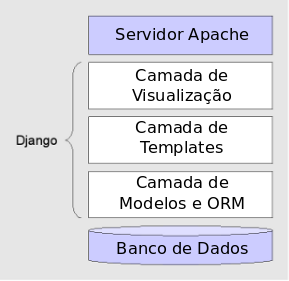
\includegraphics[width=0.9\textwidth]{../Figures/django_layers.png}}
    \caption[Diagrama com a separação entre as camadas do Django]{Nesta figura podemos observar a separação interna do Django entre as camadas de Modelo, de Visualização e de Templates. Fonte:\url{http://excess.org/article/2009/05/django-1-1-talk-text/}}
  \label{fig:django_layers2}
\end{figure}
\end{landscape}
\clearpage
}

A camada de Visualização é responsável por encapsular toda a lógica de processamento de cada requisição que é feita pelo usuário ao Django, é nesta camada onde são aplicados todos os critérios de filtragem de variantes que foram definidos pelos usuário. A camada de Modelo e ORM é responsável pelo acesso ao banco de dados através da criação de consultas em SQL que possuem os critérios de filtragem definidos pelo formulário e finalmente a camada de Templates gera o HTML final com o resultado obtido para o usuário final utilizando HTML, CSS e Javascript. 

\noindent
Site: \url{http://www.djangoproject.org}

\section{Formatos Utilizados}

\subsection{FASTQ}

O formato FASTQ foi proposto pela primeira vez em 2009 por \cite{Cock2009} e surgiu como um formato utilizado para descrever pequenas sequências de DNA chamadas de leituras (\textit{reads}) que são geradas pelos sequenciadores de DNA de nova geração. A característica principal deste formato é o armazenamento em um único arquivo da informação sobre as sequências de DNA que foram lidas e do escore de qualidade de cada base das sequências que estão presentes neste arquivo. 

A figura \ref{fig:fastq_definition} apresenta o exemplo de uma leitura em formato FASTQ. Podemos observar que cada sequência é iniciada pelo simbolo @, seguida de um ID único e com informações como o tamanho de cada leitura que foi lida pela máquina.
O simbolo ``+'' significa indica o início dos valores de qualidade de cada base na próxima linha para a leitura que foi lida anteriormente.

Existem algumas variações deste formato, como por exemplo em sequenciadores do modelo SOLID 5500XL são adicionadas informações sobre valores de qualidade de cada base em \textit{color space}. Esta tecnologia foi criada pela Applied Biosystems e chamada de \textit{2\_base encoding}, de acordo com a empresa, ela permite a leitura de cada base duas vezes sem precisar para isso realizar o sequenciamento dos dados duas vezes.

\afterpage{
\begin{landscape}
\begin{figure}[p]
  \centering
    \Large\textbf{Exemplo de uma leitura em formato FASTQ}\par\medskip   
    \fbox{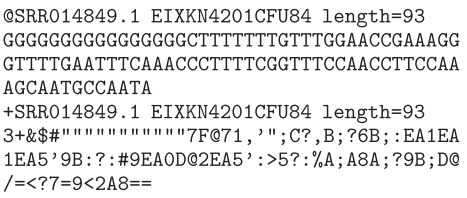
\includegraphics[width=1.5\textwidth]{./Figures/fastq_definition.png}}
    \caption[Exemplo de uma leitura em formato FASTQ]{Nesta figura podemos observar uma leitura que está presente em um arquivo no formato FASTQ. - Fonte: \cite{Cock2009} }
    
  \label{fig:fastq_definition}
\end{figure}
\end{landscape}
\clearpage
}

\subsection{Sequence Alignment Map - Formato SAM}

O formato SAM (Sequence Alignment Map) é um arquivo de texto delimitado por tabulações que foi proposto por Heng Li e Richard Dublin em 2009 \cite{Li2009b} e foi criado para armazenar as informações sobre alinhamentos de sequências como resultado após o mapeamento dessas sequências contra um genoma de referência, como por exemplo, o Genoma Humano.

A figura \ref{fig:sam_file} apresenta o exemplo de um arquivo SAM. O cabeçalho deste arquivo é delimitado pelo símbolo @ no início de cada linha, seguido de uma chave do tipo ID (Ex. HD, SQ, RG) com informações sobre como este arquivo foi gerado e os parâmetros utilizados durante o mapeamento. A segunda parte deste arquivo possui informações sobre todas as regiões mapeadas, contendo os valores de qualidade para cada base do alinhamento e um escore de qualidade médio para toda a região que foi mapeada.

O formato SAM também possui uma versão chamada de BAM, que converte os dados do arquivo SAM para uma linguagem binária (de máquina) ao invés de texto, o que ajuda a reduzir muito o tamanho do arquivo em relação ao seu original, sem que ocorra perda de informação durante essa conversão.

\afterpage{
\begin{landscape}

\begin{figure}[p]
  \centering
    \Large\textbf{Exemplo de um arquivo no formato SAM}\par\medskip   
    \fbox{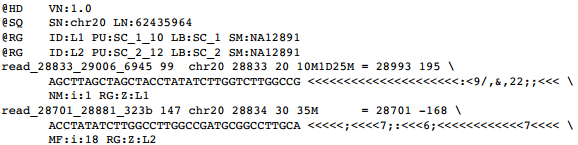
\includegraphics[width=1.5\textwidth]{./Figures/sam_file.png}}
    \caption[Exemplo de um arquivo no formato SAM]{Exemplo de um arquivo no formato SAM proposto por Li. Fonte: \cite{Li2009b}}
  \label{fig:sam_file}
\end{figure}
\end{landscape}

\clearpage
}

\subsection{Variant Call Format - Formato VCF}

O formato VCF (\textit{Variant Call Format}) foi proposto por Danecek em 2011 \cite{Danecek2011} e atualmente está em sua versão 4.2. Ele foi criado para armazenar informações sobre SNPs, Indels e Variantes Estruturais encontrados nos indivíduos sequenciados pelo projeto \textit{1000 Genomes}, juntamente com informações relevantes sobre cada variante de uma maneira compacta e indexada, usando para isso um programa desenvolvido em C chamado tabix \footnote{\url{http://www.htslib.org/doc/tabix.html}}. Este programa permite a recuperação rápida das informações genotípicas de cada indivíduo utilizando posições indexadas em relação a um genoma de referência.

A figura \ref{fig:vcf_format} apresenta um exemplo de um arquivo no formato VCF. Podemos verificar uma separação entre o cabeçalho do arquivo que é sempre iniciado com o símbolo \# e o corpo do arquivo que contém uma linha para cada variante encontrada. Este arquivo permite o armazenamento da informações do genótipo de múltiplos indivíduos, adicionando uma coluna no final do arquivo com a informação sobre o genótipo para cada indivíduo daquela posição. Todos os campos do corpo deste arquivo são separados por tabulações.

\afterpage{
\begin{landscape}

\begin{figure}[p]
  \centering
    \Large\textbf{Exemplo de um arquivo no formato VCF}\par\medskip   
    \fbox{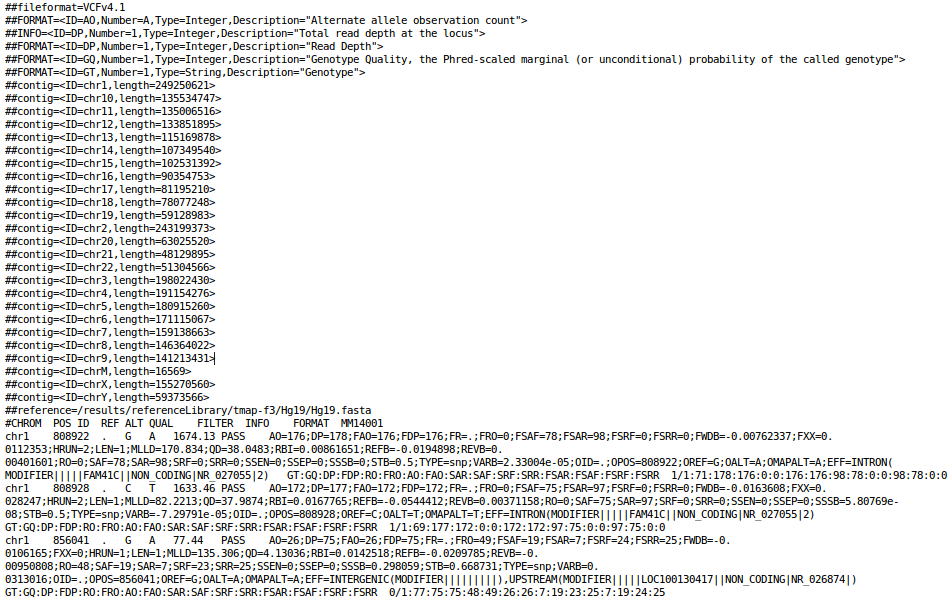
\includegraphics[width=1.2\textwidth]{./Figures/vcf_sample.png}}
    \caption[Exemplo de um arquivo no formato VCF]{Exemplo de um arquivo no formato VCF podemos observar alguns campos do cabeçalho e do corpo.}
  \label{fig:vcf_format}
\end{figure}
\end{landscape}

\clearpage
}

%adicionar o proprio vcf
% \begin{landscape}
% \lstinputlisting{data/clinical_case/vcf_header.vcf}
% \end{landscape}

\section{Programas Utilizados}

\subsection{\textit{FASTQC}}

O \textit{FASTQC} é um programa em Java que oferece uma interface gráfica para análise de dados genômicos em formato FASTQ ou BAM. Este programa permite a geração de relatórios em HTML com imagens que possuem métricas que permitem avaliar a qualidade do sequenciamento.
\noindent
Site: \url{http://www.bioinformatics.babraham.ac.uk/projects/fastqc/}


\subsection{\textit{SAMTOOLS}}

O \textit{SAMTOOLS} é um programa de linha de comando que trabalha com arquivos SAM/BAM e VCF. Além de permitir a indexação e conversão desses arquivos, este programa também possui um algoritmo Bayesiano para identificação de variantes a partir de um arquivo SAM/BAM.

\noindent
Site: \url{http://samtools.sourceforge.net/}


\subsection{\textit{PICARD TOOLS}}

O \textit{PICARD} é um programa em Java criado pelo Broad Intitute que possui ferramentas de linha de comando para a manipulação de arquivos no formato SAM/BAM. Este programa permite ordenar e indexar arquivos SAM/BAM, remover leituras que forem duplicadas, extrair métricas do alinhamento entre muitas outras coisas tarefas.

\noindent
Site: \url{http://picard.sourceforge.net}

\subsection{\textit{Burrows-Wheeler Aligner}}

O programa \textit{BWA} \cite{Li2009a} é um mapeador de leituras desenvolvido por Heng Li e  Richard Durbin que utiliza a transformada de \textit{Burrows-Wheeler} para indexar os genomas e depois realizar o processo de mapeamento das leituras contra um genoma de referência. Este alinhador foi publicado em 2009 e atualmente possui um método chamado \textit{bwa mem} que é o mais utilizado para se alinhar leituras geradas por sequenciadores da empresa Illumina. Este alinhador foi utilizado para o alinhamento do primeiro exoma recebido pelo nosso laboratório.

\noindent
Site: \url{http://bio-bwa.sourceforge.net}

\subsection{\textit{BFAST}}
O \textit{BFAST} \cite{Homer2009} acrônimo de ``BLAT-like Fast Accurate Search Tool'' é um alinhador desenvolvido por Nils Homer da Universidade da Califórnia em Los Angeles. Este programa basicamente realiza o alinhamento das leituras em duas etapas: Primeiro utilizando múltiplos índices de um genoma de referência ele identifica os locais de alinhamento candidatos para cada uma das leituras. Depois ele realiza um alinhamento com GAPs nos locais candidatos que foram identificados no passo anterior para definir aquele que possui a melhor correspondência com cada uma das leituras.

Este programa foi utilizado para a análise dos dados do sequenciador SOLID 5500XL e foi necessário a utilização de um \textit{branch} do \textit{BFAST} chamado de \textit{BFAST}+\textit{BWA} que foi recomendado pelo centro que realizou o sequenciamento dos dados, pois ele utiliza dois algoritmos diferentes para alinhar as leituras \textit{forward} e \textit{reverse} que possuem tamanhos diferentes 75 pb e 35 pb respectivamente.
\noindent
Site: \url{http://bfast.sourceforge.net}

\subsection{\textit{GATK}}

O \textit{Genome Analisys ToolKit} (\textit{GATK}) \cite{DePristo2011}  é um framework desenvolvido em Java pelo Broad Institute que possui diversos métodos utilizados para melhorar a qualidade da análise dos dados além de realizar a identificação das variantes gerando um arquivo VCF no final a partir dos arquivos SAM/BAM do alinhamento. Este programa foi utilizado para a análise de todos os dados recebidos pelo Laboratório de Genômica Clínica e também para realizar a análise dos dados do Projeto 1000Genomes. 

Um diagrama do framework proposto pelo \textit{GATK} para análise dos dados é apresentado na figura \ref{fig:gatk_framework}.

\afterpage{
\begin{landscape}

\begin{figure}[p]
  \centering
    \Large\textbf{GATK Framework de análise de variantes}\par\medskip   
    \fbox{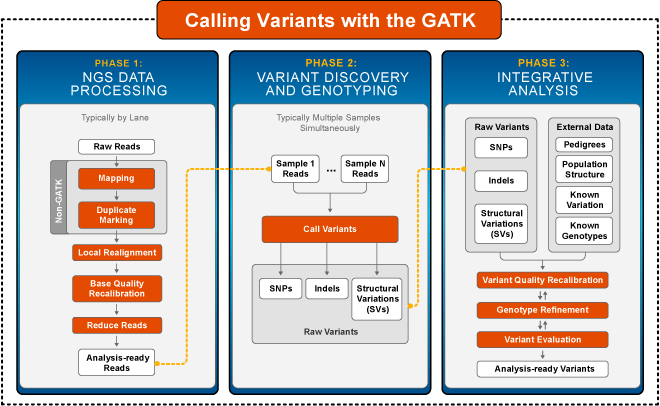
\includegraphics[width=1.4\textwidth]{../Figures/GATK.png}}
    \caption[GATK Framework de análise de variantes]{Nesta figura podemos observar todas as etapas existentes do programa \textit{GATK}. Source: https://www.broadinstitute.org/gatk/ }

  \label{fig:gatk_framework}
\end{figure}
\end{landscape}

\clearpage


}

\noindent
Site: \url{http://www.broadinstitute.org/gatk/}

\subsection{\textit{IGV}}
O \textit{IGV} é um Genome Browser desenvolvido pelo Broad Institute que permite a visualização dos dados genômicos de maneira integrativa permitindo a utilização de arquivos BAM e VCF para visualização de regiões genômicas. Este programa foi utilizado para investigação de algumas variantes candidatas identificadas por diferentes membros do nosso laboratório.
\noindent
Site: \url{http://www.broadinstitute.org/igv/}

\section{Banco de Dados e Programas Utilizadas}

\subsection{1000Genomes}

No site do projeto foi obtido um arquivo com 39.706.715 posições contendo 4 bilhões de genótipos que foram utilizadas como controle no processo de filtragem de variantes baseado em um limiar de frequência dessas variantes calculado sobre 2500 indivíduos.

Site: \url{http://www.1000genomes.org/}

\subsection{Exome Variant Server}

Esse projeto é importante pois já realizou o sequenciamento de mais de 6500 exomas de indivíduos. No site do projeto foi obtido um arquivo VCF com a frequência de 1.872.496 variantes, este arquivo é utilizado durante o processo de anotação de variantes para ajudar a filtrar variantes baseadas na sua frequência.

Site: \url{http://evs.gs.washington.edu/}

\subsection{dbSNP}

O dbSNP é um banco de dados público desenvolvido pelo National Center for Biotechnology Information (NCBI) que armazena informações sobre variações genéticas como SNPs, INDELs que foram encontradas em diferentes espécies como por exemplo: Humanos, Bovinos e Caninos. Os dados de humanos deste banco, atualmente na versão 142, foram utilizados ao longo deste projeto durante a análise dos dados e no processo de filtragem de variantes para ajudar a eliminar variantes comuns, por exemplo,  baseado na frequência dessa variante que foi encontrada em um grupo de indivíduos.

Na tabela \ref{dbsnp137} apresentamos informações sobre o último release do dbSNP versão 137.

\afterpage{
\begin{table}[p]
\captionsetup{font=normalsize}
\caption{Informações sobre o dbSNP 137}
\begin{center}
\begin{tabular}{|l|l|}
\hline
\textbf{Organismo} & Homo sapiens \\ \hline
\textbf{dbSNP Build} & 137 \\ \hline
\textbf{Genome Build} & 37.4 \\ \hline
\textbf{Número de Submissões (ss\#'s)} & 192.678.553 \\ \hline
\textbf{Número de RefSNP Clusters (rs\#'s) ( \# validados)} & 53.567.890 (38.072.522) \\ \hline
\textbf{Número de (rs\#'s) em genes} & 22.450.743 \\ \hline
\textbf{Número de (ss\#'s) com genótipo} & 75.115.460 \\ \hline
\textbf{Número de (ss\#'s) com frequência} & 35.997.781 \\ \hline
\end{tabular}
\end{center}
\label{dbsnp137}
\end{table}
\clearpage
}

Podemos observar que existem atualmente 53,567,890 \textit{reference clustered SNPIDs} (rsids), esses valores são ids únicos atribuídos a cada variante e são utilizados para anotação das frequências de cada variante.

\noindent

Site: \url{http://www.ncbi.nlm.nih.gov/projects/SNP}

\subsection{\textit{GATK Resource Bundle}}
O \textit{GATK Resource Bundle} é um repositório de arquivos recomendados pelo \textit{GATK} para serem utilizados durante a análise de genomas e exomas. Através deste repositório foram obtidos datasets com 292 exomas controles para serem utilizados no processo de filtragem de variantes.
\noindent

Site: \url{http://ftp.broadinstitute.org}

\subsection{\textit{OMIM - Online Mendelian Inheritance in Man}}

O Online Mendelian Inheritance in Man (OMIM) é um banco de dados público de genes associados a doenças Mendelianas. Este banco de dados em julho de 2015 possui 14.965 genes e 5.523  fenótipos associados a doenças Mendelianas. Essas informações foram obtidas e utilizadas para auxiliar na investigação de variantes candidatas. Por exemplo, o usuário pode buscar todos os genes associados a uma doença e visualizar as variantes desses genes presentes em cada um dos indivíduos inseridos no sistema.
\noindent

Site: \url{http://www.omim.org}

\subsection{HGNC - HUGO Gene Nomenclature Committee}

Os dados sobre os genes incluídos no Mendel,MD foram obtidos a partir do site HUGO Gene Nomenclature Committee (HGNC) \cite{Gray2013} que é um banco de dados com ``\textit{gene symbols}'' e nomes únicos para cerca de 37 mil regiões do genoma humano, sendo que mais de 19 mil dessas regiões são consideradas codificadoras de proteínas (genes). 

A tabela \ref{hgnc_genes} apresenta informações sobre os dados que foram obtidos no endereço \url{http://www.genenames.org/cgi-bin/hgnc_stats}. 

\afterpage{
\begin{table}[p]
\caption{Estatísticas sobre os genes de acordo com o HUGO \textit{Gene Nomenclature Committee} (HGNC)}
\begin{center}
\scalebox{1.0}{
\begin{tabular}{|p{1.5cm}|p{3cm}|p{5cm}|p{2cm}|}
\hline
\multicolumn{4}{|c|}{\textbf{Estatísticas sobre o Genome de Referência}} \\ \hline
\textbf{Grupo de Locus} & \textbf{Total por Grupo} & \textbf{Tipo} & \textbf{Total por Tipo de Locus} \\ \hline
\multicolumn{ 1}{|c|}{Gene codificador de proteína} & \multicolumn{ 1}{c|}{19.067} & gene com produto proteico & 19.067 \\ \hline
\multicolumn{ 1}{|c|}{RNA não-codificador} & \multicolumn{ 1}{c|}{4405} & RNA Y & 4 \\ \cline{ 3- 4}
\multicolumn{ 1}{|c|}{} & \multicolumn{ 1}{l|}{} & cluster de RNA  & 125 \\ \cline{ 3- 4}
\multicolumn{ 1}{|c|}{} & \multicolumn{ 1}{l|}{} & RNA longo não codificador & 1690 \\ \cline{ 3- 4}
\multicolumn{ 1}{|c|}{} & \multicolumn{ 1}{l|}{} & microRNA & 1524 \\ \cline{ 3- 4}
\multicolumn{ 1}{|c|}{} & \multicolumn{ 1}{l|}{} & RNA variado & 3 \\ \cline{ 3- 4}
\multicolumn{ 1}{|c|}{} & \multicolumn{ 1}{l|}{} & RNA ribossomal & 34 \\ \cline{ 3- 4}
\multicolumn{ 1}{|c|}{} & \multicolumn{ 1}{l|}{} & RNA pequeno citoplasmático & 3 \\ \cline{ 3- 4}
\multicolumn{ 1}{|c|}{} & \multicolumn{ 1}{l|}{} & RNA pequeno nuclear & 71 \\ \cline{ 3- 4}
\multicolumn{ 1}{|c|}{} & \multicolumn{ 1}{l|}{} & RNA pequeno nucleolar & 414 \\ \cline{ 3- 4}
\multicolumn{ 1}{|c|}{} & \multicolumn{ 1}{l|}{} & RNA de transferência & 533 \\ \cline{ 3- 4}
\multicolumn{ 1}{|c|}{} & \multicolumn{ 1}{l|}{} & RNA cofre & 4 \\ \hline
\multicolumn{ 1}{|c|}{Fenótipos} & \multicolumn{ 1}{c|}{703} & apenas com fenótipos & 703 \\ \hline
\multicolumn{ 1}{|c|}{Pseudogenes} & \multicolumn{ 1}{c|}{11880} & pseudogene receptor de células T & 35 \\ \cline{ 3- 4}
\multicolumn{ 1}{|c|}{} & \multicolumn{ 1}{l|}{} & pseudogene imunoglobulina & 199 \\ \cline{ 3- 4}
\multicolumn{ 1}{|c|}{} & \multicolumn{ 1}{l|}{} & pseudogene & 11.646 \\ \hline
\multicolumn{ 1}{|c|}{Outros} & \multicolumn{ 1}{c|}{1111} & gene do receptor de células T & 207 \\ \cline{ 3- 4}
\multicolumn{ 1}{|c|}{} & \multicolumn{ 1}{l|}{} & constituinte de locus complexo & 27 \\ \cline{ 3- 4}
\multicolumn{ 1}{|c|}{} & \multicolumn{ 1}{l|}{} & retrovírus endógeno & 73 \\ \cline{ 3- 4}
\multicolumn{ 1}{|c|}{} & \multicolumn{ 1}{l|}{} & sítio frágil & 117 \\ \cline{ 3- 4}
\multicolumn{ 1}{|c|}{} & \multicolumn{ 1}{l|}{} & genes de imunoglobulina & 224 \\ \cline{ 3- 4}
\multicolumn{ 1}{|c|}{} & \multicolumn{ 1}{l|}{} & protocaderina & 39 \\ \cline{ 3- 4}
\multicolumn{ 1}{|c|}{} & \multicolumn{ 1}{l|}{} & leitura & 86 \\ \cline{ 3- 4}
\multicolumn{ 1}{|c|}{} & \multicolumn{ 1}{l|}{} & região & 44 \\ \cline{ 3- 4}
\multicolumn{ 1}{|c|}{} & \multicolumn{ 1}{l|}{} & elemento transponível & 4 \\ \cline{ 3- 4}
\multicolumn{ 1}{|c|}{} & \multicolumn{ 1}{l|}{} & desconhecidos & 282 \\ \cline{ 3- 4}
\multicolumn{ 1}{|c|}{} & \multicolumn{ 1}{l|}{} & local de integração de vírus & 8 \\ \hline
\multicolumn{ 3}{|c|}{\textbf{Total de símbolos aprovados}} & 37.166 \\ \hline
\end{tabular}
}
\end{center}
\label{hgnc_genes}
\end{table}
\clearpage
}

Site: \url{http://www.genenames.org}

\subsection{HGMD}

O HGMD \cite{Stenson2009} é um banco de dados comercial com mutações germinativas e nucleares que foram descritas e validadas pela literatura como sendo associadas a doenças humanas. Estes dados foram utilizados para permitir a busca de mutações que já estivessem descritas anteriormente pela literatura.

Site: \url{http://www.hgmd.cf.ac.uk}

\subsection{Genoma Humano de Referência b37}

Todas as análises deste trabalho foram realizadas usando a versão b37 do genoma humano, o mesmo arquivo que foi utilizado pelo projeto 1000genomes para suas análises e está disponível no repositório ``\textit{GATK Resource Bundle}'' no FTP do Broad Institute. Ele seria o equivalente ao hg19 do genoma fornecido pelo UCSC.

A tabela \ref{b37_chrs} apresenta o número de pares de base em cada um dos 84 contigs referentes aos cromossomos além dos contigs que ainda não puderam ser incorporados nos cromossomos. Os contigs iniciados com GL (Genome Library) são sequências que ainda não puderam ser integradas aos contigs canônicos (ex. 1,2,3)
 
\afterpage{
\begin{table}[p]
\caption{Tabela com informações sobre o número de pares de bases de cada um dos cromossomos do genome build b37.}
%     \begin{center}
	\centering
    \begin{tabular}{|l|l|l|l|}
    \hline
    Contig          & Pares de Base & Contig & Pares de Base  \\ \hline
    1          & 249.250.621 & GL000208.1 & 92.689  \\ \hline
    2          & 243.199.373 & GL000209.1 & 159.169 \\ \hline
    3          & 198022.430 & GL000210.1 & 27.682  \\ \hline
    4          & 191.154.276 & GL000211.1 & 166.566 \\ \hline
    5          & 180.915.260 & GL000212.1 & 186.858 \\ \hline
    6          & 171.115.067 & GL000213.1 & 164.239 \\ \hline
    7          & 159.138.663 & GL000214.1 & 137.718 \\ \hline
    8          & 146.364.022 & GL000215.1 & 172.545 \\ \hline
    9          & 141.213.431 & GL000216.1 & 172.294 \\ \hline
    10         & 135.534.747 & GL000217.1 & 172.149 \\ \hline
    11         & 135.006.516 & GL000218.1 & 161.147 \\ \hline
    12         & 133.851.895 & GL000219.1 & 179.198 \\ \hline
    13         & 115.169.878 & GL000220.1 & 161.802 \\ \hline
    14         & 107.349.540 & GL000221.1 & 155.397 \\ \hline
    15         & 102.531.392 & GL000222.1 & 186.861 \\ \hline
    16         & 90.354.753  & GL000223.1 & 180.455 \\ \hline
    17         & 81.195.210  & GL000224.1 & 179.693 \\ \hline
    18         & 78.077.248  & GL000225.1 & 211.173 \\ \hline
    19         & 59.128.983  & GL000226.1 & 15.008  \\ \hline
    20         & 63.025.520  & GL000227.1 & 128.374 \\ \hline
    21         & 48.129.895  & GL000228.1 & 129.120 \\ \hline
    22         & 51.304.566  & GL000229.1 & 19.913  \\ \hline
    X          & 155.270.560 & GL000230.1 & 43.691  \\ \hline
    Y          & 59.373.566  & GL000231.1 & 27.386  \\ \hline
    MT         & 16.569     & GL000232.1 & 40.652  \\ \hline
    GL000191.1 & 106.433    & GL000233.1 & 45.941  \\ \hline
    GL000192.1 & 547.496    & GL000234.1 & 40.531  \\ \hline
    GL000193.1 & 189.789    & GL000235.1 & 34.474  \\ \hline
    GL000194.1 & 191.469    & GL000236.1 & 41.934  \\ \hline
    GL000195.1 & 182.896    & GL000237.1 & 45.867  \\ \hline
    GL000196.1 & 38.914     & GL000238.1 & 39.939  \\ \hline
    GL000197.1 & 37.175     & GL000239.1 & 33.824  \\ \hline
    GL000198.1 & 90.085     & GL000240.1 & 41.933  \\ \hline
    GL000199.1 & 169.874    & GL000241.1 & 42.152  \\ \hline
    GL000200.1 & 187.035    & GL000242.1 & 43.523  \\ \hline
    GL000201.1 & 36.148     & GL000243.1 & 43.341  \\ \hline
    GL000202.1 & 40.103     & GL000244.1 & 39.929  \\ \hline
    GL000203.1 & 37.498     & GL000245.1 & 36.651  \\ \hline
    GL000204.1 & 81.310     & GL000246.1 & 38.154  \\ \hline
    GL000205.1 & 174.588    & GL000247.1 & 36.422  \\ \hline
    GL000206.1 & 41.001     & GL000248.1 & 39.786  \\ \hline
    GL000207.1 & 4.262      & GL000249.1 & 38.502  \\ \hline
    \end{tabular}
% \end{center}

\label{b37_chrs}
\end{table}
\clearpage
}


Site: \url{ftp://ftp-trace.ncbi.nih.gov/1000genomes/ftp/technical/reference/}


\subsection{Escore PHRED}

O escore de qualidade chamado PHRED (Q) é um valor entre 4 e 60 que é dado para cada base de DNA que é lida de acordo com a sua qualidade utilizando uma escala negativa de probabilidade do log dos valores de qualidade. Esse valor é calculado de acordo com a seguinte fórmula:

\[Q=-10\log_{10}P\]

Como exemplo, um phred escore de 10 significa que temos a probabilidade de 1 erro a cada 10 bases, ou seja 90\% de acurácia para cada base que foi lida, já um Phred escore de 60 indica a probabilidade de erro de 1 em 1.000.000 milhão de bases ou seja 99.99999\% de acurácia.

Site: \url{http://www.phrap.com/phred/}

\subsection{Escore SIFT}

O SIFT \cite{Ng2003} é um escore criado para predizer o impacto causado na função da proteína por mudanças na sua sequência de aminoácidos. Esse escore é bastante utilizado para ajudar a identificar boas variantes candidatas. Esse algoritmo utiliza homologia de sequências para predizer se uma substituição do aminoácido pode causar uma mudança na estrutura de uma determinada proteína. Apesar de seu primeiro artigo ter sido publicado em 2001 ainda é bastante utilizado na análise de exomas.

\url{http://sift.jcvi.org/}

\subsection{Escore Polyphen-2}

Esse é um escore de patogenicidade que também é bastante utilizado, porém sua diferença em relação ao SIFT é que quanto maior for o escore mais patogênica tende a ser a variante estudada \cite{Adzhubei2013}. Portanto, valores próximos de 1.0 seriam mais patogênicos de acordo com esse algoritmo.

\url{http://genetics.bwh.harvard.edu/pph2/}

\subsection{Escore CADD}
 
O CADD (\textit{Combined Annotation Dependent Depletion}) é um escore que integra múltiplas anotações em uma única métrica utilizando mutações que sobrevivem a um processo de seleção natural aplicado sobre mutações simuladas ao longo do genoma \cite{Kircher2014a}. Esse escore pode ser utilizado para encontrar mutações patogênicas, porém ao contrário dos escores de SIFT e Polyphen-2, ele não possui valores sugeridos para determinar se uma variante é ou não é patogênica, quanto maior o seu valor maior a chance da variante ser patogênica.

\url{http://cadd.gs.washington.edu/}


\subsection{\textit{SnpEff}}

O \textit{SnpEff} é uma ferramenta para anotação e predição do efeito causado por variantes presentes em diversas regiões de um genoma. Além de realizar a anotação de SNPs e indels que estão localizados nos genes, ele também é capaz de predizer mutações em regiões de \textit{splicing}, regiões com \textit{frameshifts}, perda ou ganho de função entre outras que estão descritas no site da ferramenta.

Na tabela \ref{snpeff_faq} podemos observar que a maioria dos efeitos das variantes que podem causar problemas pertencem as classes HIGH ou MODERATE classificadas por este programa. Estas duas categorias podem ser utilizadas como critério de filtragem durante a análise de exomas para identificação de possíveis genes e mutações candidatas.


\begin{table}[]
\Large 
\centering
\caption{Tabela com as classes de impacto do programa SnpEff}
\label{snpeff_faq}
\scalebox{0.6}{
\begin{tabular}{|l|l|lll}
\cline{1-2}
\textbf{Impacto} & \textbf{Termo Ontológico}                                  &  &  &  \\ \cline{1-2}
HIGH                           & chromosome\_number\_variation                        &  &  &  \\ \cline{1-2}
HIGH                           & exon\_loss\_variant                                  &  &  &  \\ \cline{1-2}
HIGH                           & frameshift\_variant                                  &  &  &  \\ \cline{1-2}
HIGH                           & rare\_amino\_acid\_variant                           &  &  &  \\ \cline{1-2}
HIGH                           & splice\_acceptor\_variant                            &  &  &  \\ \cline{1-2}
HIGH                           & splice\_donor\_variant                               &  &  &  \\ \cline{1-2}
HIGH                           & start\_lost                                          &  &  &  \\ \cline{1-2}
HIGH                           & stop\_gained                                         &  &  &  \\ \cline{1-2}
HIGH                           & stop\_lost                                           &  &  &  \\ \cline{1-2}
HIGH                           & transcript\_ablation                                 &  &  &  \\ \cline{1-2}
MODERATE                       & 3\_prime\_UTR\_truncation +exon\_loss                &  &  &  \\ \cline{1-2}
MODERATE                       & 5\_prime\_UTR\_truncation +exon\_loss\_variant       &  &  &  \\ \cline{1-2}
MODERATE                       & coding\_sequence\_variant                            &  &  &  \\ \cline{1-2}
MODERATE                       & disruptive\_inframe\_deletion                        &  &  &  \\ \cline{1-2}
MODERATE                       & disruptive\_inframe\_insertion                       &  &  &  \\ \cline{1-2}
MODERATE                       & inframe\_deletion                                    &  &  &  \\ \cline{1-2}
MODERATE                       & inframe\_insertion                                   &  &  &  \\ \cline{1-2}
MODERATE                       & missense\_variant                                    &  &  &  \\ \cline{1-2}
MODERATE                       & regulatory\_region\_ablation                         &  &  &  \\ \cline{1-2}
MODERATE                       & splice\_region\_variant                              &  &  &  \\ \cline{1-2}
MODERATE                       & TFBS\_ablation                                       &  &  &  \\ \cline{1-2}
LOW                            & 5\_prime\_UTR\_premature start\_codon\_gain\_variant &  &  &  \\ \cline{1-2}
LOW                            & initiator\_codon\_variant                            &  &  &  \\ \cline{1-2}
LOW                            & splice\_region\_variant                              &  &  &  \\ \cline{1-2}
LOW                            & start\_retained                                      &  &  &  \\ \cline{1-2}
LOW                            & stop\_retained\_variant                              &  &  &  \\ \cline{1-2}
LOW                            & synonymous\_variant                                  &  &  &  \\ \cline{1-2}
MODIFIER                       & 3\_prime\_UTR\_variant                               &  &  &  \\ \cline{1-2}
MODIFIER                       & 5\_prime\_UTR\_variant                               &  &  &  \\ \cline{1-2}
MODIFIER                       & coding\_sequence\_variant                            &  &  &  \\ \cline{1-2}
MODIFIER                       & conserved\_intergenic\_variant                       &  &  &  \\ \cline{1-2}
MODIFIER                       & downstream\_gene\_variant                            &  &  &  \\ \cline{1-2}
MODIFIER                       & conserved\_intron\_variant                           &  &  &  \\ \cline{1-2}
MODIFIER                       & exon\_variant                                        &  &  &  \\ \cline{1-2}
MODIFIER                       & feature\_elongation                                  &  &  &  \\ \cline{1-2}
MODIFIER                       & feature\_truncation                                  &  &  &  \\ \cline{1-2}
MODIFIER                       & gene\_variant                                        &  &  &  \\ \cline{1-2}
MODIFIER                       & intergenic\_region                                   &  &  &  \\ \cline{1-2}
MODIFIER                       & intragenic\_variant                                  &  &  &  \\ \cline{1-2}
MODIFIER                       & intron\_variant                                      &  &  &  \\ \cline{1-2}
MODIFIER                       & mature\_miRNA\_variant                               &  &  &  \\ \cline{1-2}
MODIFIER                       & miRNA                                                &  &  &  \\ \cline{1-2}
MODIFIER                       & NMD\_transcript\_variant                             &  &  &  \\ \cline{1-2}
MODIFIER                       & non\_coding\_transcript\_exon\_variant               &  &  &  \\ \cline{1-2}
MODIFIER                       & non\_coding\_transcript\_variant                     &  &  &  \\ \cline{1-2}
MODIFIER                       & regulatory\_region\_amplification                    &  &  &  \\ \cline{1-2}
MODIFIER                       & regulatory\_region\_variant                          &  &  &  \\ \cline{1-2}
MODIFIER                       & TF\_binding\_site\_variant                           &  &  &  \\ \cline{1-2}
MODIFIER                       & TFBS\_amplification                                  &  &  &  \\ \cline{1-2}
MODIFIER                       & transcript\_amplification                            &  &  &  \\ \cline{1-2}
MODIFIER                       & transcript\_variant                                  &  &  &  \\ \cline{1-2}
MODIFIER                       & upstream\_gene\_variant                              &  &  &  \\ \cline{1-2}
\end{tabular}
}
\end{table}

\noindent
Site: \url{http://snpeff.sourceforge.net}

\subsection{\textit{ANNOVAR}}

O \textit{ANNOVAR} \cite{Wang2010} é um software de anotação genômica que utiliza informações atualizadas de bancos de dados como o 1000Genomes, dbSNP137 e ESP6500 além de ferramentas como SIFT, Polyphen-2, Phylop e Mutation Taster de uma maneira integrada e rápida  para anotar arquivos no formato VCF através de scripts desenvolvidos em Perl.

\noindent
Site: \url{http://www.openbioinformatics.org/annovar}


\subsection{dbNSFP}

O dbNSFP \cite{Liu2011b} é um banco de dados que integra anotações funcionais de diversos algoritmos de predição de variantes e possui cerca de ~75 milhões de SNPs não-sinônimas em sua base de dados. Ele utiliza escores de diferentes ferramentas de predição (Ex. SIFT, Polyphen-2, LRT, MutationTaster e MutationAssessor) e escores de conservação (PhyloP, GERP++ e SiPhy) para o processo de anotação de variantes.

\noindent
Site: \url{http://sites.google.com/site/jpopgen/dbNSFP}

\section{Workflow de Análise de Exomas}

Para análise dos exomas recebidos foi necessário o desenvolvimento de um workflow utilizando os programas: \textit{BWA}, \textit{SAMTOOLS}, \textit{Piccard} e \textit{GATK}.

Este pipeline foi inicialmente desenvolvido em Bash e executado no supercomputador do CENAPAD-MG sendo posteriormente transformado em um script em python para permitir a sua execução no servidor do laboratório, facilitando a integração com os outros scripts desenvolvidos.

A seguir apresentamos um diagrama com o nosso pipeline implementado de acordo com o guia de melhores práticas oferecido pelo site do \textit{GATK} no endereço: \url{http://www.broadinstitute.org/gatk/guide/article?id=15}

Na figura \ref{fig:exome_pipeline} podemos visualizar um diagrama com todas as etapas e os processos utilizados neste pipeline:

\afterpage{
\begin{landscape}

\begin{figure}[p]
  \centering
    \Large\textbf{Diagrama com o pipeline de análise de exomas}\par\medskip   
    \fbox{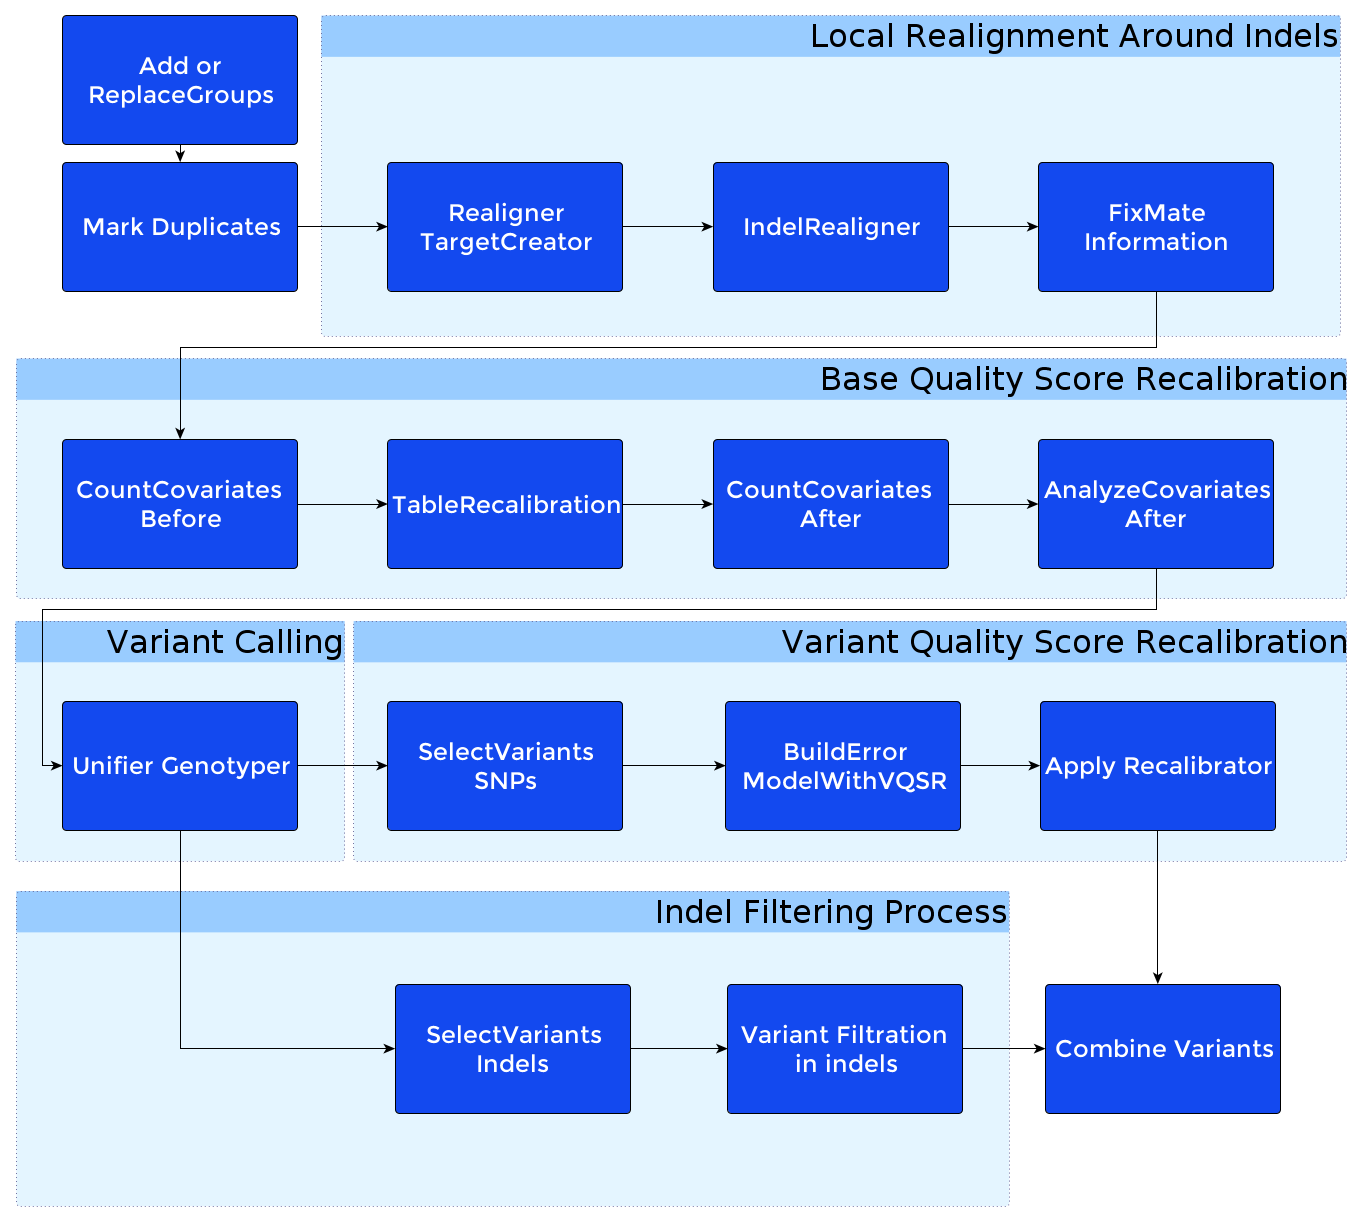
\includegraphics[width=0.9\textwidth]{../Diagramas/gatk_pipelinev2.png}}
    \caption[Diagrama com o pipeline de análise de exomas]{Pipeline desenvolvido para realizar a análise de exomas utilizando o \textit{GATK}. Nesta figura é possivel observar que existem subetapas dentro de cada etapa proposta pelo GATK.}
    
  \label{fig:exome_pipeline}
\end{figure}
\end{landscape}

\clearpage
}

Além do \textit{GATK} outros programas que aceitam arquivos BAMs como entrada foram utilizados para identificação de CNVs e  Short Tandem Repeats (STRs) \cite{Gymrek2012,Krumm2012a,Li2012}.

\subsection{Alinhamento dos dados de SOLID 5500xl}

Para dos dados do sequenciador SOLID 5500xl foi necessário o desenvolvimento de um novo pipeline utilizando uma versão modificada do alinhador \textit{BFAST} que possui uma implementação do \textit{BWA} para alinhar leituras curtas. As leituras deste sequenciador possuem tamanhos diferentes sendo 75 pb para a sequência forward e 35 pb para a sequência reverse, portanto cada uma precisa ser alinhada com um algoritmo diferente. Este alinhador foi recomendado pelo Sick Children Hospital de Toronto que é o lugar onde os dados foram gerados.

%Metodologia
\chapter{Resultados}

\section{Alinhamento e Análise de Exomas}

No dia 6 de outubro de 2011 foi recebido o primeiro exoma para ser analisado pelo Laboratório de Genômica Clínica (LGC) na Faculdade de Medicina da UFMG em Belo Horizonte.

O sequenciamento desse exoma foi realizado utilizando um sequenciador modelo Illumina HiSeq2000, utilizando o kit de enriquecimento para captura das regiões exônicas desenvolvido pela Roche NimbleGen versão SeqCap EZ Human Exome Library v2 (44.1 Mbp) e foi dada uma garantia de cobertura mínima de pelo menos 30 vezes (30X) pela empresa Otogenetics que realizou o sequenciamento do DNA deste paciente.

Após o recebimento dos dois arquivos em formato FASTQ.GZ nós utilizamos o programa FASTQC para verificar a quantidade de leituras e obter métricas em relação aos valores de qualidade das leituras deste indivíduo.

\subsection{Controle de Qualidade sobre os dados}

Esses dois arquivos FASTQ continham 35.701.713 \textit{leituras} cada um, totalizando 71.403.426 de ``\textit{leituras paired-end}'', essas leituras estavam codificadas com um escore phred de qualidade no formato Illumina 1.5+ e tiveram que ser convertidas para o formato Sanger de qualidade para se tornarem compatíveis com o programa GATK. Cada leitura possui 90 nucleotídeos de tamanho tanto para as sequências \textit{forward} quanto as \textit{reverse} e o conteúdo médio GC dessas sequências foi de 44\%. Este valor está próximo do valor de 50\% que seria o esperado para as regiões exônicas do genoma humano. Um valor muito alto ou muito baixo de GC poderia indicar que houve algum tipo de problema com o enriquecimento dessas regiões.

Na tabela \ref{rms_seq} são apresentadas informações sobre as sequências forward e reverse que foram obtidas utilizando o programa FASTQC. Esses arquivos é o que chamamos de dados brutos (``\textit{raw data}''), pois são os dados que saíram diretamente do sequenciador e ainda não foram analisados ou alterados por nenhum tipo de programa.

\afterpage{

\begin{landscape}

\begin{table}[!htb]
    \caption{Métricas sobre as Sequências \textit{forward} e \textit{reverse} do indivíduo RMS}
    \label{rms_seq}
    \begin{subtable}{.5\linewidth}
      \centering
        \caption{Forward}
        \scalebox{1.3}{
	  \begin{tabular}{|l|l|}
	  \hline
	  \multicolumn{1}{|c|}{\textbf{Medida}} & \multicolumn{1}{c|}{\textbf{Valor}} \\ \hline
	  Tipo de Arquivo & Conventional base calls \\ \hline
	  Codificação & Illumina 1.5 \\ \hline
	  Total de Sequências & 35.701.713 \\ \hline
	  Sequências Filtradas & 0 \\ \hline
	  Tamanho das Sequências & 90 \\ \hline
	  \%GC & 44 \\ \hline
	  \end{tabular}
	}
    \end{subtable}%
    \begin{subtable}{.5\linewidth}
      \centering
        \caption{Reverse}
        \scalebox{1.3}{
        \begin{tabular}{|l|l|}
	\hline
	\multicolumn{1}{|c|}{\textbf{Medida}} & \multicolumn{1}{c|}{\textbf{Valor}} \\ \hline
	Tipo de Arquivo & Conventional base calls \\ \hline
	Codificação & Illumina 1.5 \\ \hline
	Total de Sequências & 35.701.713 \\ \hline
	Sequências Filtradas & 0 \\ \hline
	Tamanho das Sequências & 90 \\ \hline
	\%GC & 44 \\ \hline
	\end{tabular}
	}
    \end{subtable} 
\end{table}

\end{landscape}


\clearpage
}

A seguir são apresentadas imagens com informações sobre a qualidade das leituras. Podemos observar que esses dados estão com um valor ótimo de qualidade e não possuem nenhum desvio significativo em relação aos valores que seriam esperados.

Na figura \ref{fig:per_base_sequence_quality} podemos observar que a qualidade das bases ao longo das leituras possui em média um \textit{phred escore} acima de 30 e notamos que a partir do meio da leitura até o seu final existe uma leve redução dos valores de qualidade, isto geralmente acontece com dados de sequenciadores Illumina.

A figura \ref{fig:per_sequence_quality} mostra a qualidade média das leituras e podemos observar que os valores de qualidade estão entre 37 e 38 tanto para a sequência forward quanto para a sequência reverse. Este resultado pode ser considerado bom, caso contrário esta imagem poderia indicar algum tipo de problema ocorrido durante o sequenciamento.

Na figura \ref{fig:per_base_sequence_content} apresentamos a distribuição dos nucleotídeos A, C, T e G ao longo das leituras e podemos observar que a quantidade de nucleotídeos A e T foi maior do que a quantidade de nucleotídeos G e C. Isso é esperado e pode ser considerado normal desde que a diferença entre esses dois grupos não ultrapasse 20\%.


\afterpage{
\begin{landscape}

\begin{figure}
\centering
\Large\textbf{Escore \textit{Phred} de qualidade médio por base das sequências do indivíduo RMS}\par\medskip   
\begin{subfigure}{.75\textwidth}
  \centering
  \fbox{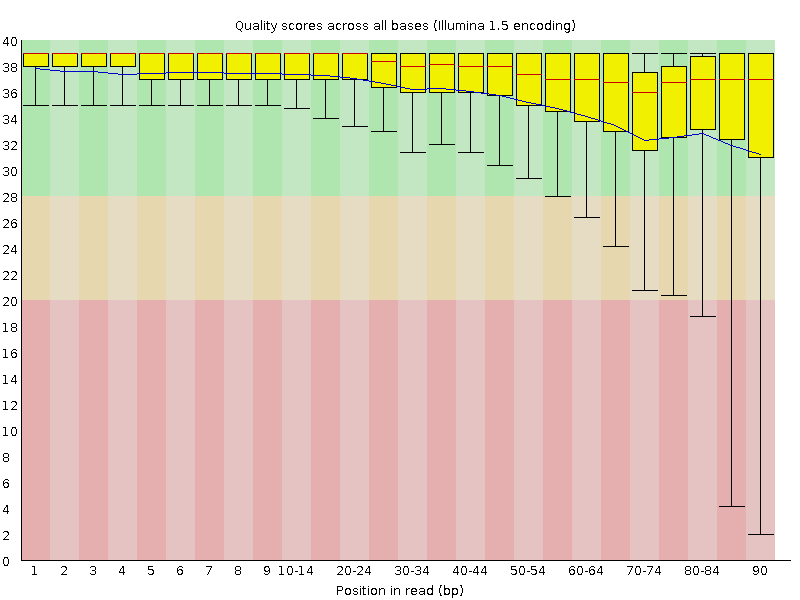
\includegraphics[width=0.9\linewidth]{../Figures/Ot729_index7_Exome_Sergio.Pena_RDNP_07262011-reads1-110716_I123_FCC043NABXX_L2_index7_1_fastqc/Images/per_base_quality.png}}
  \caption{Sequências Forward}
\end{subfigure}%
\begin{subfigure}{.75\textwidth}
  \centering
  \fbox{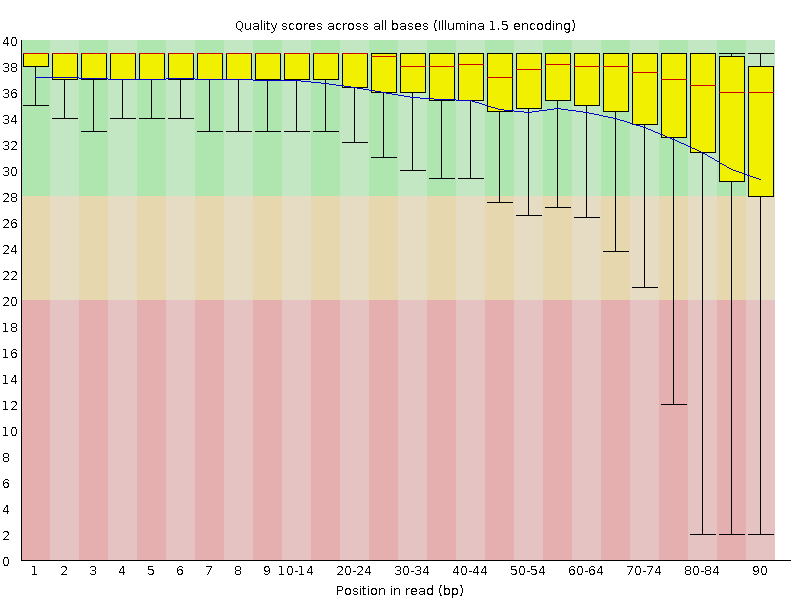
\includegraphics[width=0.9\linewidth]{../Figures/Ot729_index7_Exome_Sergio.Pena_RDNP_07262011-reads2-110716_I123_FCC043NABXX_L2_index7_2_fastqc/Images/per_base_quality.png}}
  \caption{Sequências Reverse}
\end{subfigure}
\caption[Escore \textit{Phred} de qualidade médio por base das sequências do indivíduo RMS]{Podemos observar que o score phred de qualidade das bases ficou sempre acima de 30, havendo uma pequena degradação no final das reads, o que é bastante característico de dados provenientes da plataforma illumina.}
\label{fig:per_base_sequence_quality}
\end{figure}

\begin{figure}
\centering
\Large\textbf{Distribuição do Escore \textit{Phred} em relação a todas as sequências do indivíduo RMS}\par\medskip   
\begin{subfigure}{.75\textwidth}
  \centering
  \fbox{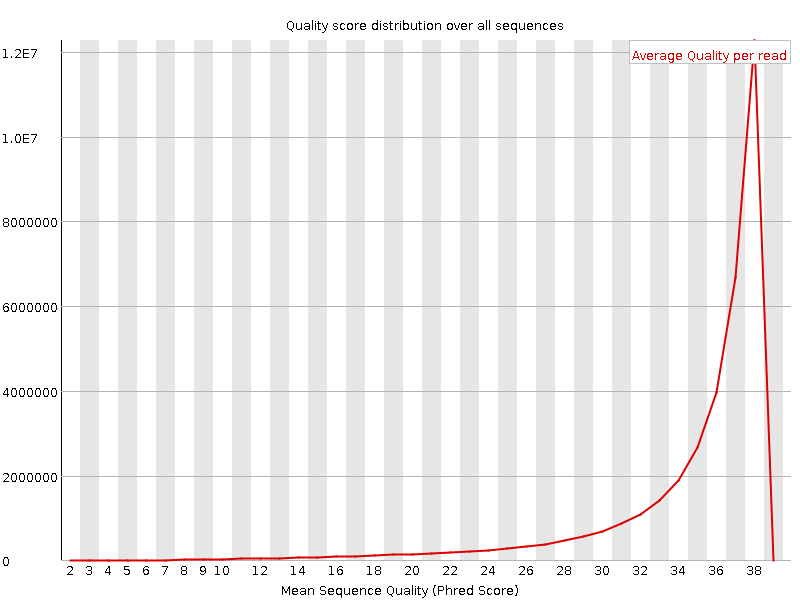
\includegraphics[width=0.9\linewidth]{../Figures/Ot729_index7_Exome_Sergio.Pena_RDNP_07262011-reads1-110716_I123_FCC043NABXX_L2_index7_1_fastqc/Images/per_sequence_quality.png}}
  \caption{Sequências Forward}

\end{subfigure}%
\begin{subfigure}{.75\textwidth}
  \centering
  \fbox{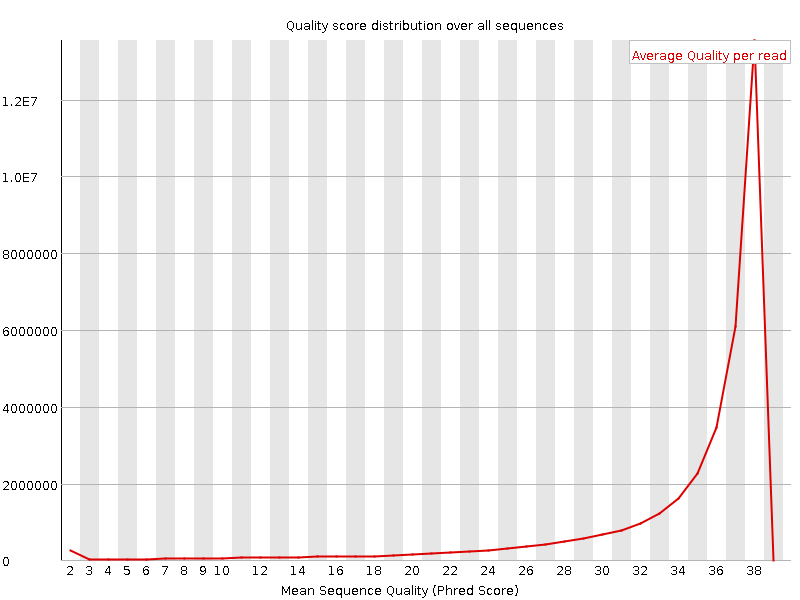
\includegraphics[width=0.9\linewidth]{../Figures/Ot729_index7_Exome_Sergio.Pena_RDNP_07262011-reads2-110716_I123_FCC043NABXX_L2_index7_2_fastqc/Images/per_sequence_quality.png}}
  \caption{Sequências Reverse}

\end{subfigure}
\caption[Distribuição do Escore \textit{Phred} em relação a todas as sequências do indivíduo RMS]{Podemos observar que o phred escore médio de qualidade para as reads forward e reverse foram de 38.}
\label{fig:per_sequence_quality}
\end{figure}

\begin{figure}
\centering
\Large\textbf{Conteúdo de sequência por base para as sequências do indivíduo RMS}\par\medskip
\begin{subfigure}{.75\textwidth}
  \centering
  \fbox{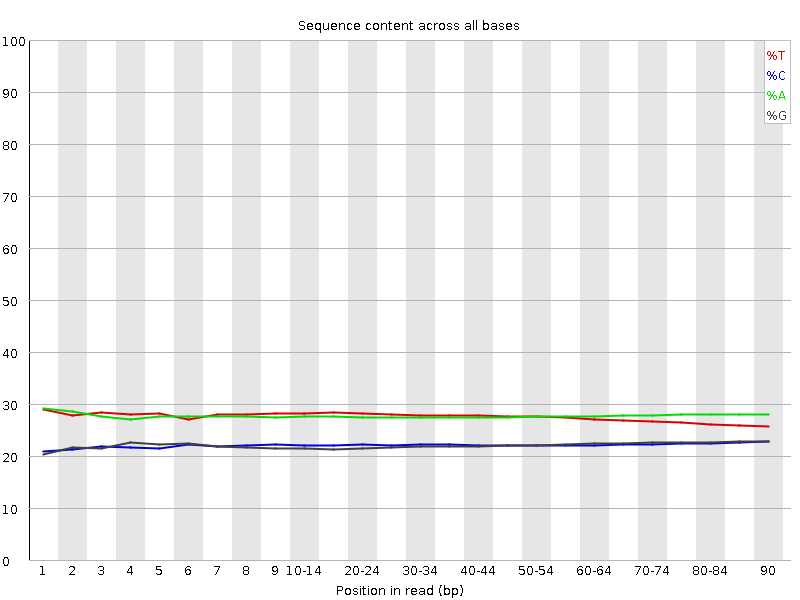
\includegraphics[width=0.9\linewidth]{../Figures/Ot729_index7_Exome_Sergio.Pena_RDNP_07262011-reads1-110716_I123_FCC043NABXX_L2_index7_1_fastqc/Images/per_base_sequence_content.png}}
  \caption{Sequências Forward}
\end{subfigure}%
\begin{subfigure}{.75\textwidth}
  \centering
  \fbox{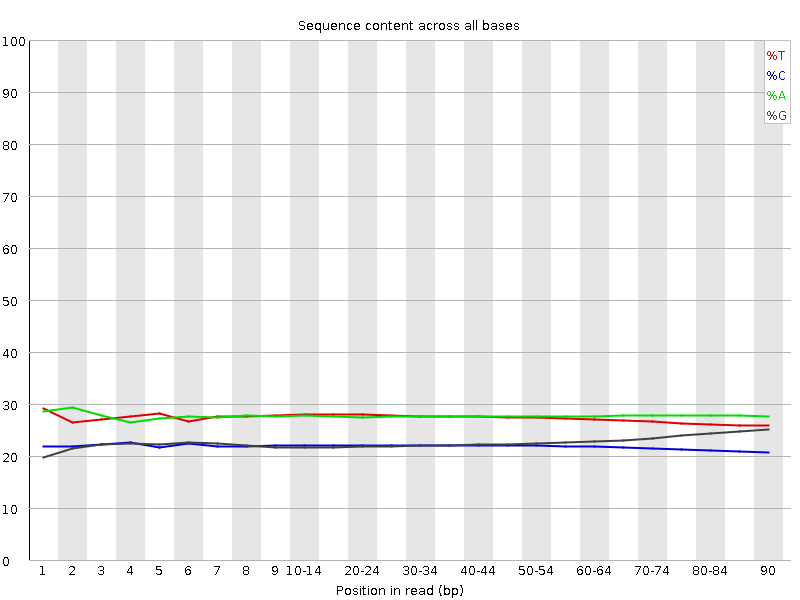
\includegraphics[width=0.9\linewidth]{../Figures/Ot729_index7_Exome_Sergio.Pena_RDNP_07262011-reads2-110716_I123_FCC043NABXX_L2_index7_2_fastqc/Images/per_base_sequence_content.png}}
  \caption{Sequências Reverse}
\end{subfigure}
\caption[Conteúdo de sequência por base para as sequências do indivíduo RMS]{Nesta figura podemos observar a distribuição de cada uma das bases A, C, T, e G ao longo das reads.}
\label{fig:per_base_sequence_content}
\end{figure}

\end{landscape}

}

Na figura \ref{fig:gc_content_per_sequence} podemos observar a distribuição do conteúdo GC para todas as sequências e que esse valor foi em média 44\%. A linha em azul representa o modelo teórico de distribuição que seria esperado. Podemos afirmar que o valor real aproxima-se bastante do valor esperado e caso estas distribuições fossem diferentes isso poderia indicar um problema de contaminação da amostra com outros organismos.

Na figura \ref{fig:duplication_levels} apresentamos os níveis de duplicação das sequência e podemos observar valores de duplicação de 39.79\% e 38.73\% para as sequências, o que pode ser considerado baixo. Um alto nível de duplicação indica que houve um enriquecimento de certas sequências, Um baixo nível de duplicação indica uma alta cobertura das regiões presentes no alvo.

Na figura \ref{fig:kmer_profiles} apresentamos os perfis de kmer das 6 sequências mais comuns com tamanho 5 nucleotídeos (5mer) ao longo das leituras. Podemos afirmar que não houve um enriquecimento relativo muito alto entre os 6 kmers mais frequentes das sequências. Caso o enriquecimento de um kmer fosse por exemplo 3X maior em relação aos outros isto poderia indicar um problema com o sequenciamento.


\afterpage{
\begin{landscape}

\begin{figure}
\centering
\Large\textbf{Distribuição do conteúdo de GC nas leituras}\par\medskip
\begin{subfigure}{.7\textwidth}
  \centering
  \fbox{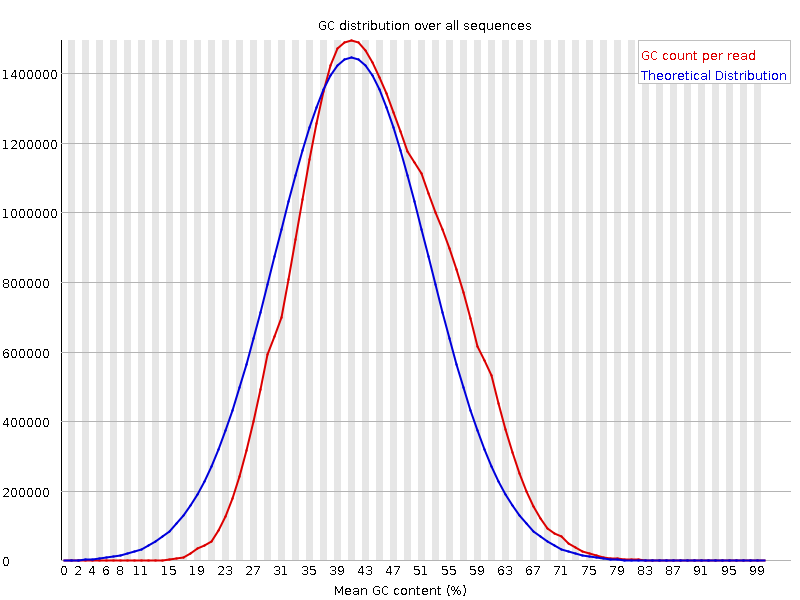
\includegraphics[width=0.9\linewidth]{../Figures/Ot729_index7_Exome_Sergio.Pena_RDNP_07262011-reads1-110716_I123_FCC043NABXX_L2_index7_1_fastqc/Images/per_sequence_gc_content.png}}
  \caption{Sequências Forward}
\end{subfigure}%
\begin{subfigure}{.7\textwidth}
  \centering
  \fbox{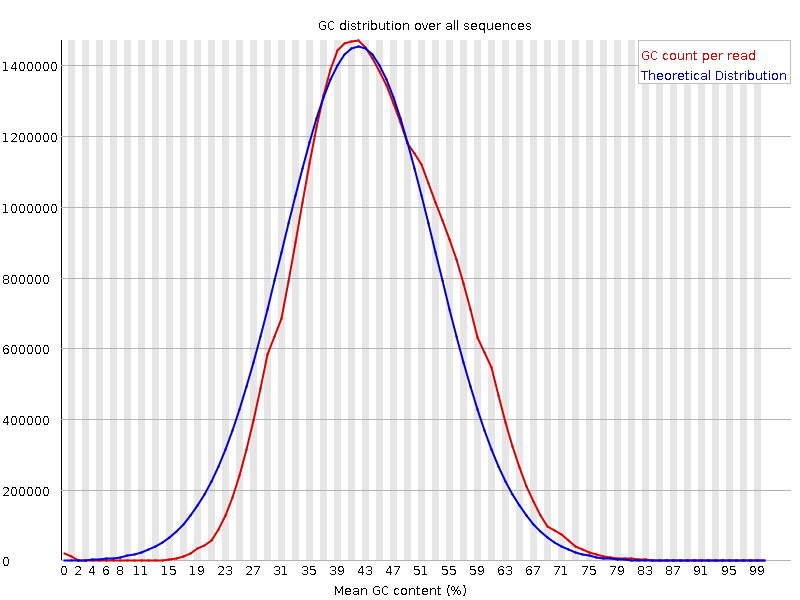
\includegraphics[width=0.9\linewidth]{../Figures/Ot729_index7_Exome_Sergio.Pena_RDNP_07262011-reads2-110716_I123_FCC043NABXX_L2_index7_2_fastqc/Images/per_sequence_gc_content.png}}
  \caption{Sequências Reverse}
\end{subfigure}
\caption[Distribuição do conteúdo de GC nas leituras]{Nesta figura podemos observar a distribuição do conteúdo GC ao longo das leituras.}
\label{fig:gc_content_per_sequence}
\end{figure}

\begin{figure}
\centering
\Large\textbf{Níveis de duplicação}\par\medskip
\begin{subfigure}{.7\textwidth}
  \centering
  \fbox{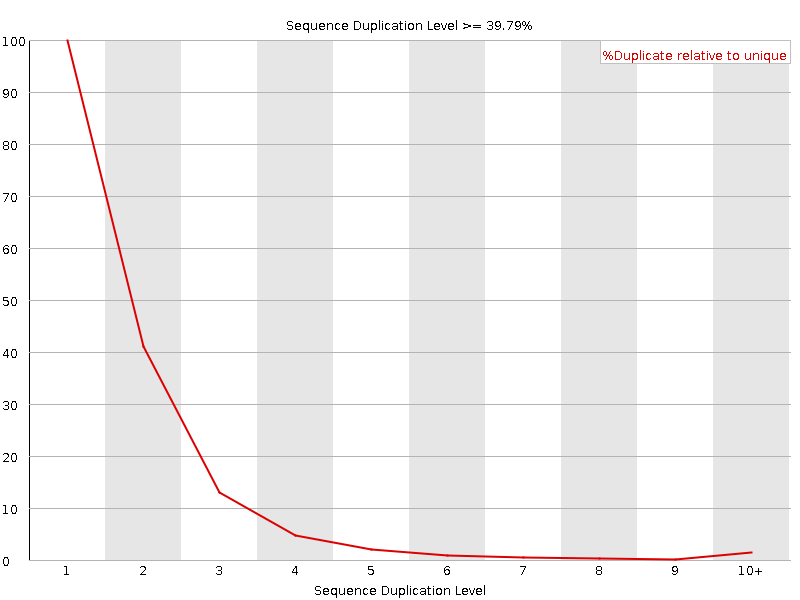
\includegraphics[width=0.9\linewidth]{../Figures/Ot729_index7_Exome_Sergio.Pena_RDNP_07262011-reads1-110716_I123_FCC043NABXX_L2_index7_1_fastqc/Images/duplication_levels.png}}
  \caption{Sequências Forward}
\end{subfigure}%
\begin{subfigure}{.7\textwidth}
  \centering
  \fbox{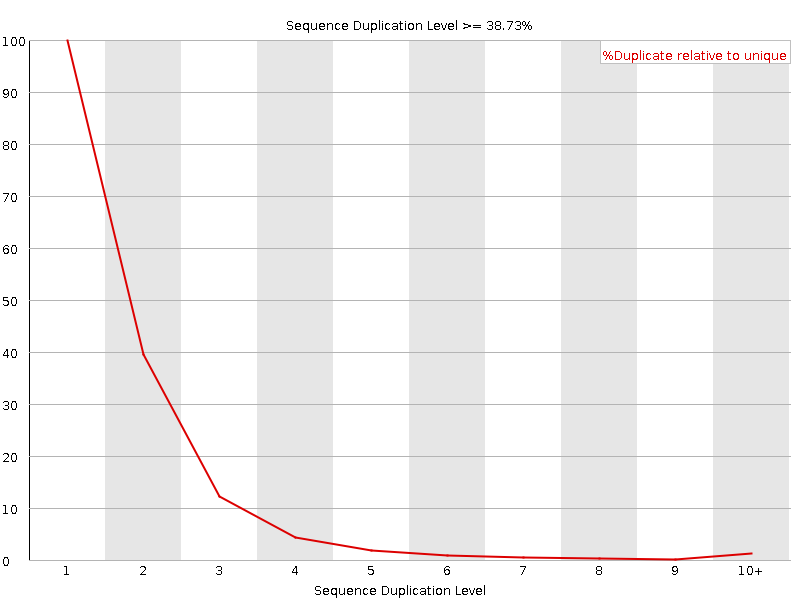
\includegraphics[width=0.9\linewidth]{../Figures/Ot729_index7_Exome_Sergio.Pena_RDNP_07262011-reads2-110716_I123_FCC043NABXX_L2_index7_2_fastqc/Images/duplication_levels.png}}
  \caption{Sequências Reverse}
\end{subfigure}
\caption[Níveis de duplicação]{Nesta figura podemos obersar os níveis de duplicação. Uma quantidade alta do nível de duplicação pode indicar um problema com o sequenciamento.}
\label{fig:duplication_levels}
\end{figure}

\begin{figure}
\centering
\Large\textbf{Perfis de K-mer}\par\medskip
\begin{subfigure}{.7\textwidth}
  \centering
  \fbox{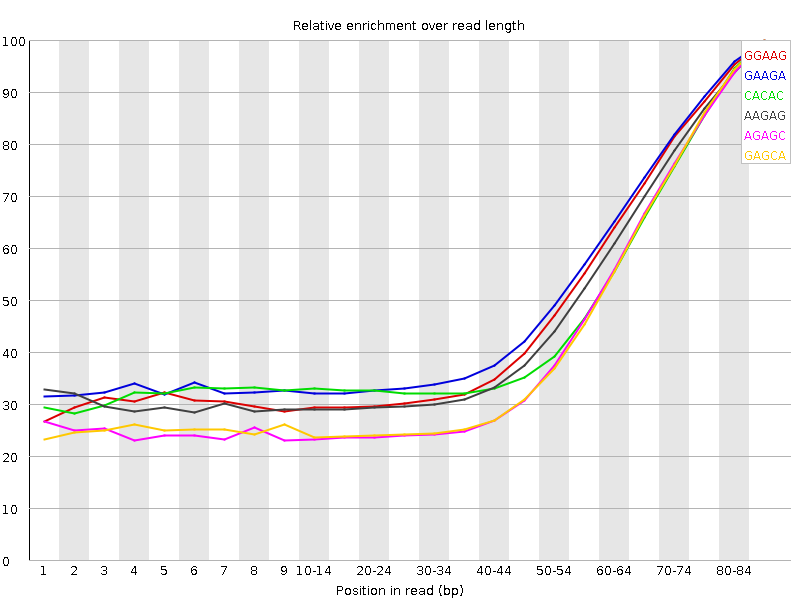
\includegraphics[width=0.9\linewidth]{../Figures/Ot729_index7_Exome_Sergio.Pena_RDNP_07262011-reads1-110716_I123_FCC043NABXX_L2_index7_1_fastqc/Images/kmer_profiles.png}}
  \caption{Sequências Forward}
\end{subfigure}%
\begin{subfigure}{.7\textwidth}
  \centering
  \fbox{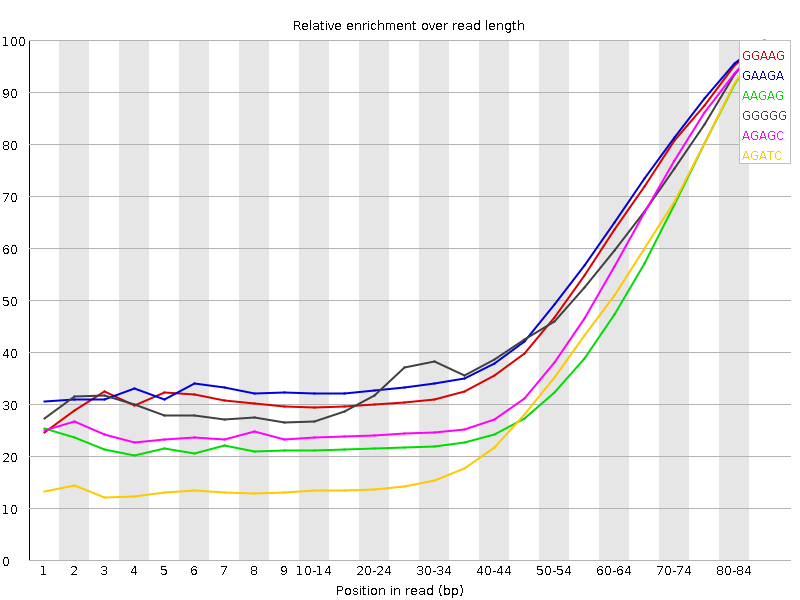
\includegraphics[width=0.9\linewidth]{../Figures/Ot729_index7_Exome_Sergio.Pena_RDNP_07262011-reads2-110716_I123_FCC043NABXX_L2_index7_2_fastqc/Images/kmer_profiles.png}}
  \caption{Sequências Reverse}
\end{subfigure}
\caption[Perfis de K-mer]{Nesta figura podemos observar o enriquecimento relativo do número de kmers ao longo das leituras, um desbalanceamento grande de um kmer específico pode indicar um problema com o sequenciamento.}
\label{fig:kmer_profiles}
\end{figure}

\end{landscape}

}

Antes de realizar o alinhamento foi necessário converter o escore de codificação das sequências do formato Illumina 1.5 para o formato Sanger utilizando um script em perl fornecido pelo programa MAQ (\url{http://maq.sourceforge.net/fq_all2std.pl}). Esta conversão é necessária para a análise dos dados utilizando o GATK.

\subsection{Alinhamento}

Após verificação da qualidade dos dados recebidos, foi feito um alinhamento utilizando o alinhador BWA que mapeou as leituras contra a versão b37 do genoma humano de referência.

Ao final deste mapeamento foi obtido um arquivo BAM como resultado e então foram extraídas métricas de qualidade sobre este alinhamento com o programa samstat. Este programa foi útil para ajudar a verificar métricas sobre a qualidade do alinhamento em arquivos do tipo BAM antes e depois de utilizarmos o GATK para melhorar a qualidade e corrigir alguns problemas nesses arquivos.

A seguir é apresentado um resumo do que aconteceu com os dados durante a execução do GATK dentro do pipeline de análise de exomas desenvolvido por este trabalho e apresentado na figura \ref{fig:exome_pipeline} na parte de Métodos.

\subsection{GATK Genome Analysis ToolKit}

Após o alinhamento com o BWA nós utilizamos o programa GATK para melhorar a qualidade das leituras e realizar o processo chamado de \textit{``calling das variantes''}. Para calcular a cobertura média do exoma, foi utilizado o programa bedtools \footnote{\url{https://github.com/arq5x/bedtools}} que procura por regiões definidas pelo kit de sequenciamento utilizado. O arquivo BED com os targets para este exoma foram obtidos no link: \href{http://www.nimblegen.com/products/seqcap/ez/v2/}{http://www.nimblegen.com/products/seqcap/ez/v2/}

Nas figuras~\ref{fig:rms_before_gatkv1} e~\ref{fig:rms_before_gatkv2} podemos observar um sumário sobre a qualidade do alinhamento das leituras antes de utilizarmos o GATK. Tivemos aproximadamente 71.4 milhões de leituras mapeadas e além disso 75\% dessas leituras tiveram um escore de alinhamento MAPQ acima de 30 o que pode ser considerado um resultado muito bom para este tipo de análise.

Nas figuras~\ref{fig:rms_after_gatkv1} e~\ref{fig:rms_after_gatkv2} apresentamos um sumário sobre o alinhamento depois que o GATK foi utilizado. Embora o número de leituras tenha diminuído em relação a figura anterior, nota-se um aumento no valor da qualidade na região final das leituras presentes.

\afterpage{
\begin{figure}[p]
\centering
\Large\textbf{Estatísticas do alinhamento antes de utilizarmos o GATK}\par\medskip
\fbox{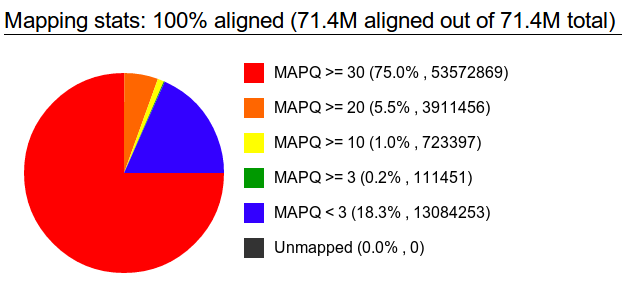
\includegraphics[width=0.9\textwidth]{alinhamento_rms/antes_gatk_summary.png}}
\caption[Estatísticas do alinhamento antes de utilizarmos o GATK]{Nesta figura podemos observar que o alinhamento obteve mais de 75\% das leituras com escore de phred maior do que 30.} \label{fig:rms_before_gatkv1}

\Large\textbf{Qualidade média por base do alinhamento antes de utilizarmos o GATK}\par\medskip
\fbox{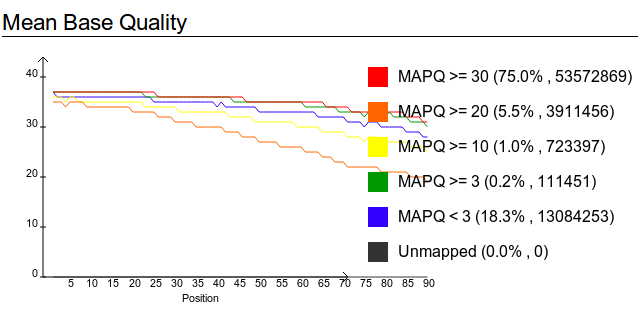
\includegraphics[width=0.9\textwidth]{alinhamento_rms/antes_gatk_mean_base_quality.png}}
\caption[Qualidade média por base do alinhamento antes de utilizarmos o GATK]{Nesta figura podemos observar a distribuição da qualidade ao longo das bases para cada grupo de leituras do alinhamento.} \label{fig:rms_before_gatkv2}
\end{figure}
\clearpage
}

\afterpage{
\begin{figure}[p]
\centering
\Large\textbf{Estatísticas do alinhamento depois de utilizarmos o GATK}\par\medskip
\fbox{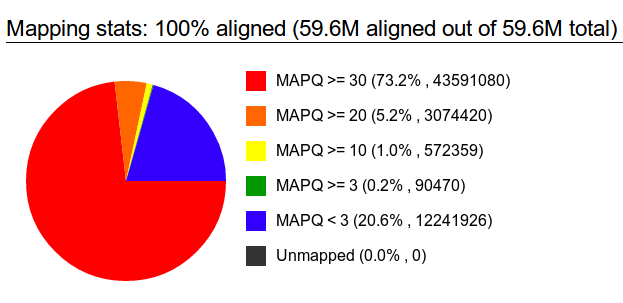
\includegraphics[width=0.9\textwidth]{alinhamento_rms/rms_after_gatk_mapping_stats.png}}
\caption[Estatísticas do alinhamento depois de utilizarmos o GATK]{Nesta figura podemos observar uma redução do número total de leituras devido a remoção de leituras com baixa qualidade dentro de cada um dos grupos.} \label{fig:rms_after_gatkv1}

\Large\textbf{Qualidade média por base do alinhamento depois de utilizarmos o GATK}\par\medskip
\fbox{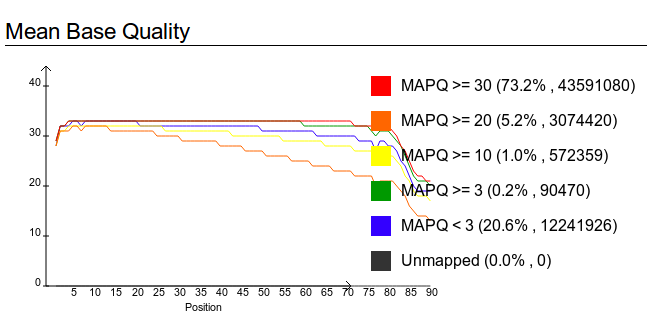
\includegraphics[width=0.9\textwidth]{alinhamento_rms/rms_after_gatk_mean_base_quality.png}}
\caption[Qualidade média por base do alinhamento depois de utilizarmos o GATK]{Nesta figura podemos observar uma estratificação maior da qualidade das leituras após a filtragem das leituras com baixa qualidade.} \label{fig:rms_after_gatkv2}
\end{figure}
\clearpage
}

\subsubsection{Remoção de leituras duplicadas}

Primeiro foi utilizado o comando MarkDuplicates para remover leituras duplicadas em nosso arquivo de alinhamento, durante este processo 17\% das leituras foram consideradas duplicadas e foram descartadas. Este passo é importante pois ajuda a reduzir os erros na hora de realizarmos o \textit{``calling das variantes''}. Esta remoção não diminui a cobertura do sequenciamento mas ajuda a melhorar a qualidade das áreas que foram cobertas. Ao final restaram 59.570.255 milhões de leituras passaram para a próxima etapa.

Na tabela \ref{aln_after_dedup} apresentamos um resumo detalhado das leituras contidas no arquivo de alinhamento após este processo.

\afterpage{
\begin{table}[p]
\caption{Informações sobre o alinhamento após a remoção de leituras duplicadas}
\begin{center}
\begin{tabular}{|l|l|}
\hline
no total (leituras que passaram no controle de qualidade) & 59.570.255 \\ \hline
mapeadas (84.31\% do total) & 50.222.733 \\ \hline
pareadas no sequenciamento & 59.570.255 \\ \hline
leitura1 & 29.756.446 \\ \hline
leitura2 & 29.813.809 \\ \hline
corretamente pareadas (80.78\%) & 48.122.446 \\ \hline
com ela própria e com a companheira mapeada & 49.778.115 \\ \hline
únicas (0.75\%) & 444.618 \\ \hline
com a leitura companheira mapeada em um cromossomo diferente & 112.890 \\ \hline
com a leitura companheira mapeada em um cromossomo diferente (mapQ>=5) & 66.095 \\ \hline
\end{tabular}
\end{center}
\label{aln_after_dedup}
\end{table}
\clearpage
}

\subsubsection{Realinhamento Local em regiões de Indels}

\subsubsubsection{Criação dos alvos para realinhamento}

Este método realiza uma busca ao longo do alinhamento por regiões que possuam características específicas como SNPs presentes no final das leituras que sejam discordantes para as leituras \textit{forward} e \textit{reverse} ou que estejam em regiões com repetição de nucleotídeos, por exemplo (TTTTT). Então, ele marca estas regiões para que um realinhamento local seja realizado utilizando o método de Smith–Watermann com o objetivo de corrigir possíveis erros gerados durante o alinhamento dessas sequências e encontrar indels nesta região.

A seguir apresentamos o resultado da saída deste método:

\begin{itemize}
  \item Tempo de execução 5719.67 segundos, 95.33 minutos, 1.59 horas.
  \item 3.611.533 leituras foram filtradas durante o processo de um total de 51.194.954 (7,05 \%).
  \item 3.611.499 leituras (7.05\% do total) falharam o filtro de qualidade zero de mapeamento.
  \item 34 leituras (0.00\% do total) falharam o filtro de leituras não mapeadas.
\end{itemize}


\subsubsubsection{Aplicação da Recalibração}

Este método realiza um realinhamento local nas leituras selecionadas pelo passo anterior para tentar melhorar a posição das leituras em relação a regiões com indels. Por exemplo, quando temos uma indel verdadeira que foi mapeada contra o genoma de referência, as leituras próximas a essa indel estarão mapeadas incorretamente se a região de início ou fim da leitura estiver próxima ao indel.

Após este processo o comando FixMate do programa Picard foi utilizado para remover as leituras órfãs, ou seja aquelas que o seu par tenha sido descartado durante este processo.

\subsubsection{Recalibração do Escore de Qualidade da Base}

Após o realinhamento de indels o GATK possui uma etapa de recalibração dos escores de qualidade. Este processo avalia a maneira como cada leitura varia em relação as outras leituras com o objetivo de deixar os valores mais uniformes e corrigir um possível viés de cada tecnologia.

A seguir apresentamos gráficos mostrando o que acontece com os dados antes e depois deste processo.

\afterpage{
\begin{landscape}

\begin{figure}
\centering
\Large\textbf{Escore de Qualidade Empírico vs Reportado}\par\medskip
\begin{subfigure}{.7\textwidth}
  \centering
  \fbox{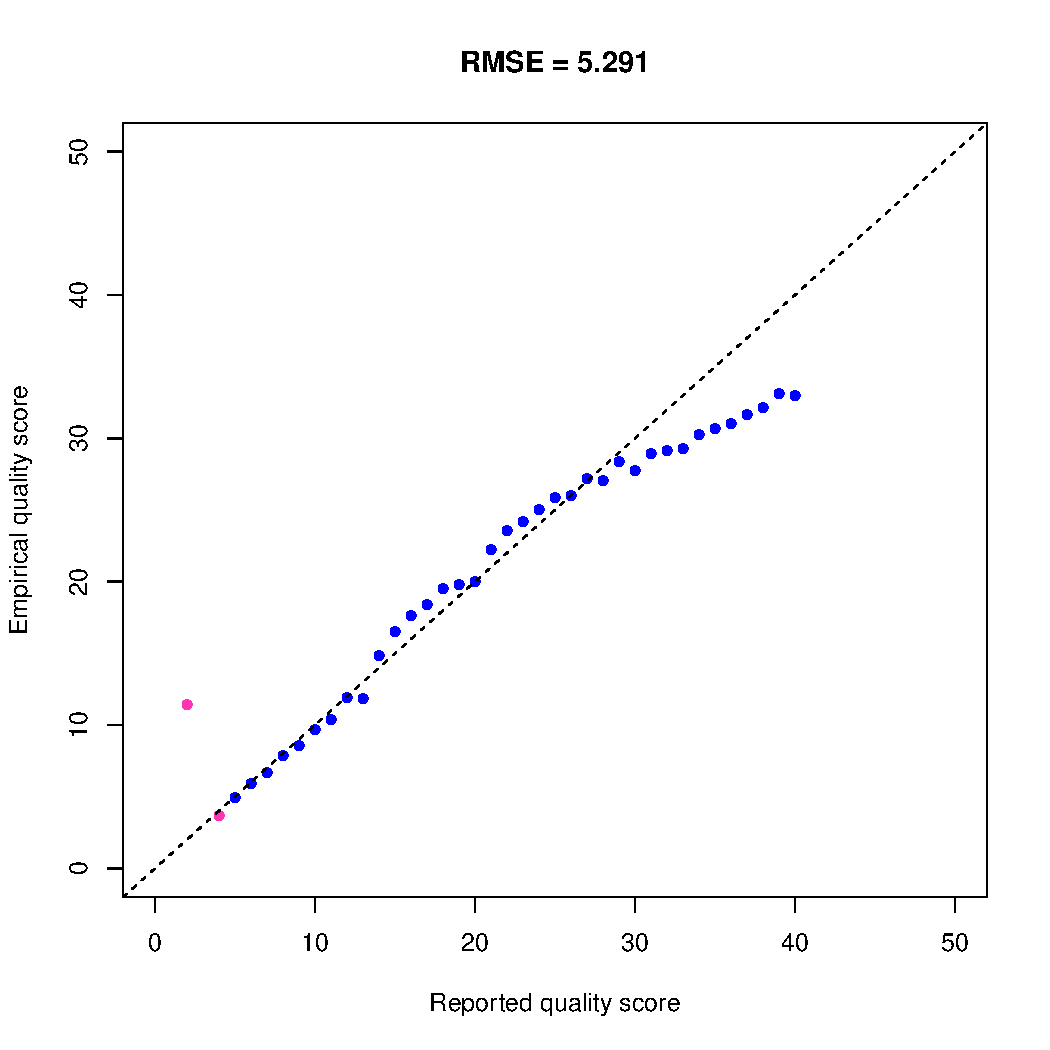
\includegraphics[width=0.9\linewidth]{alinhamento_rms/exome.sorted.dedup.real.fixed.recal.stats.before/emp_v_stated.pdf}}
  \caption{Antes da recalibração do escore de qualidade}
\end{subfigure}%
\begin{subfigure}{.7\textwidth}
  \centering
  \fbox{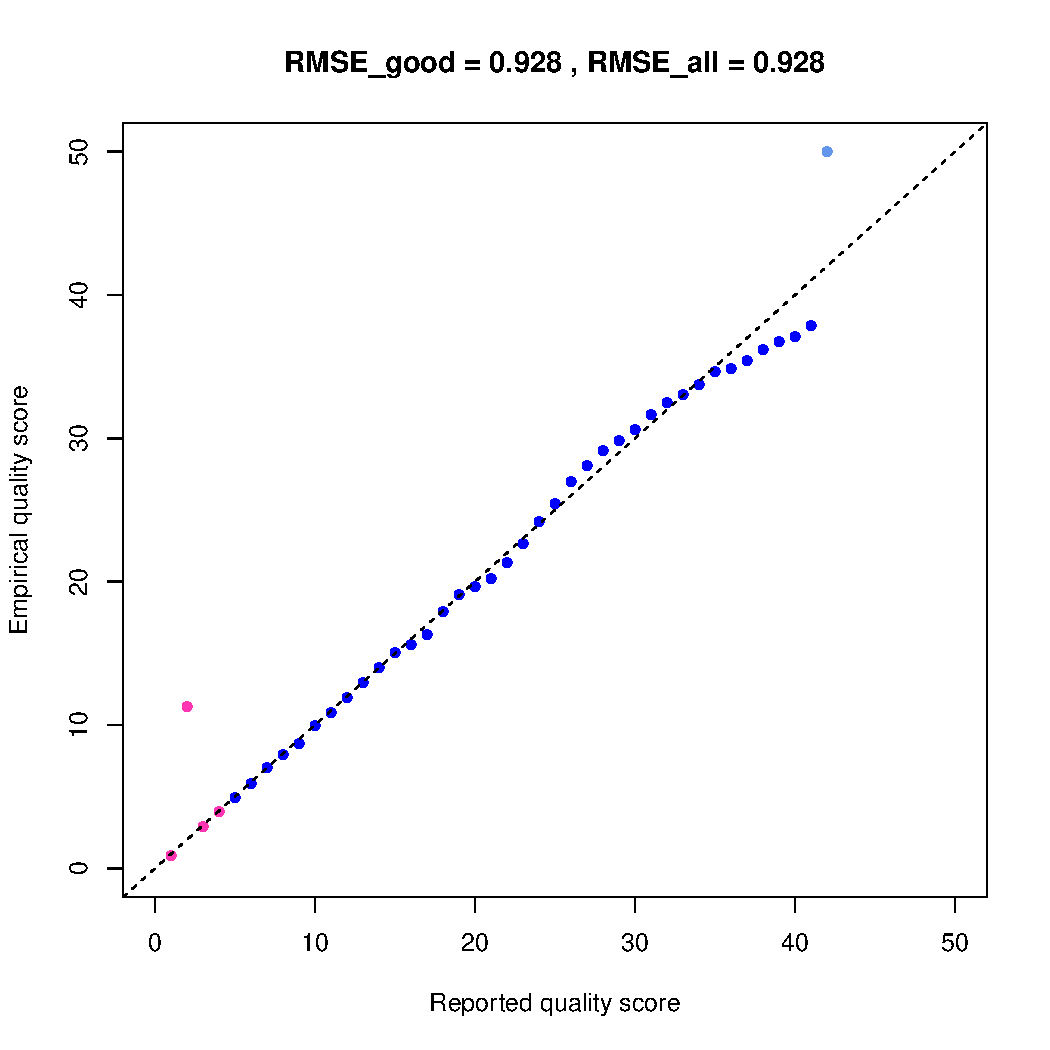
\includegraphics[width=0.9\linewidth]{alinhamento_rms/exome.sorted.dedup.real.fixed.recal.stats.after/emp_v_stated.pdf}}
  \caption{Depois da recalibração do escore de qualidade}
\end{subfigure}
\caption[Escore de Qualidade Empírico vs Reportado]{Nesta figura podemos observar uma estratificação maior do escore de qualidade, este processo ajudar a corrigir um viés que existe no escore de qualidade de acordo com cada plataforma.}
\label{fig:rms_before_emp_v_stated}
\end{figure}

\begin{figure}
\centering
\Large\textbf{Número de Bases vs Escore de Qualidade}\par\medskip
\begin{subfigure}{.7\textwidth}
  \centering
  \fbox{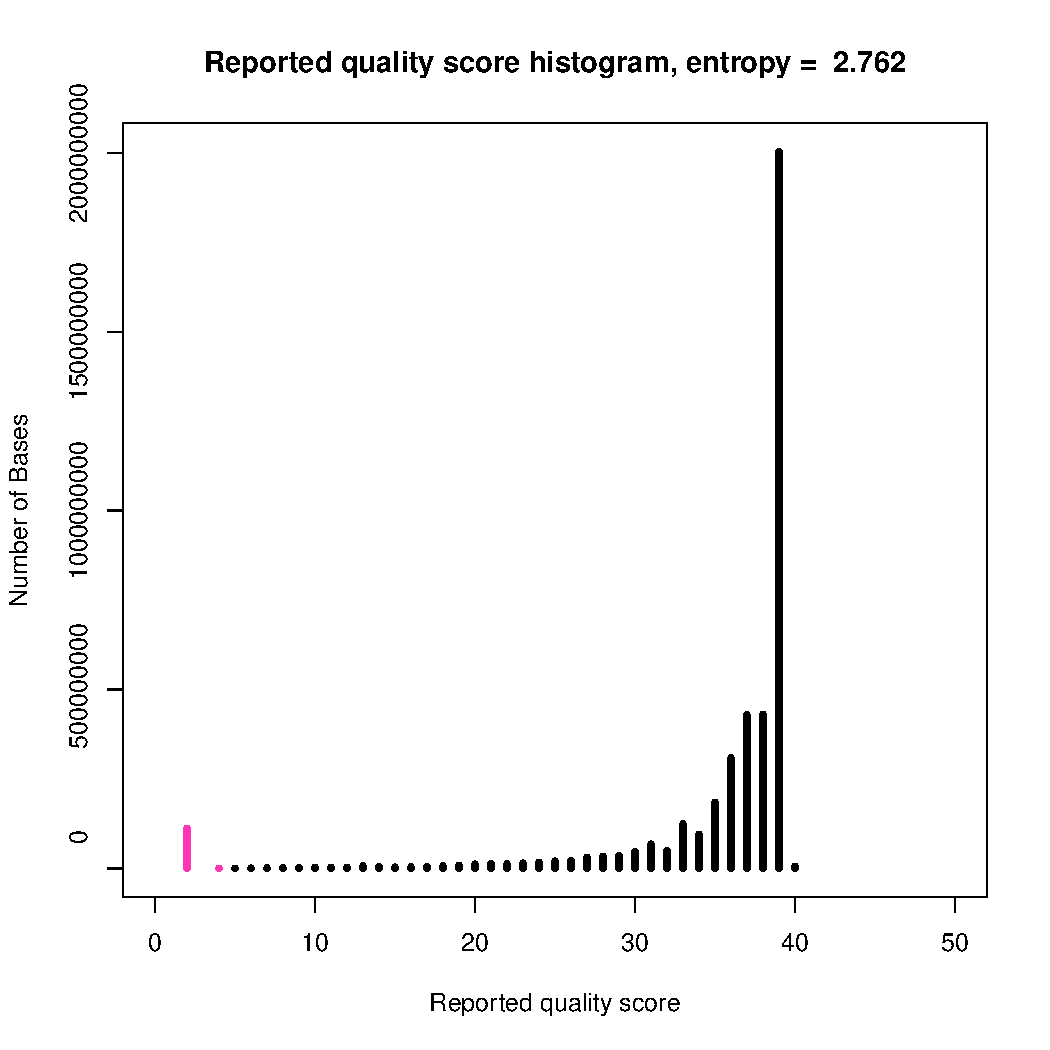
\includegraphics[width=0.9\linewidth]{alinhamento_rms/exome.sorted.dedup.real.fixed.recal.stats.before/quality_rep_hist.pdf}}
  \caption{Antes da recalibração do escore de qualidade}
\end{subfigure}%
\begin{subfigure}{.7\textwidth}
  \centering
  \fbox{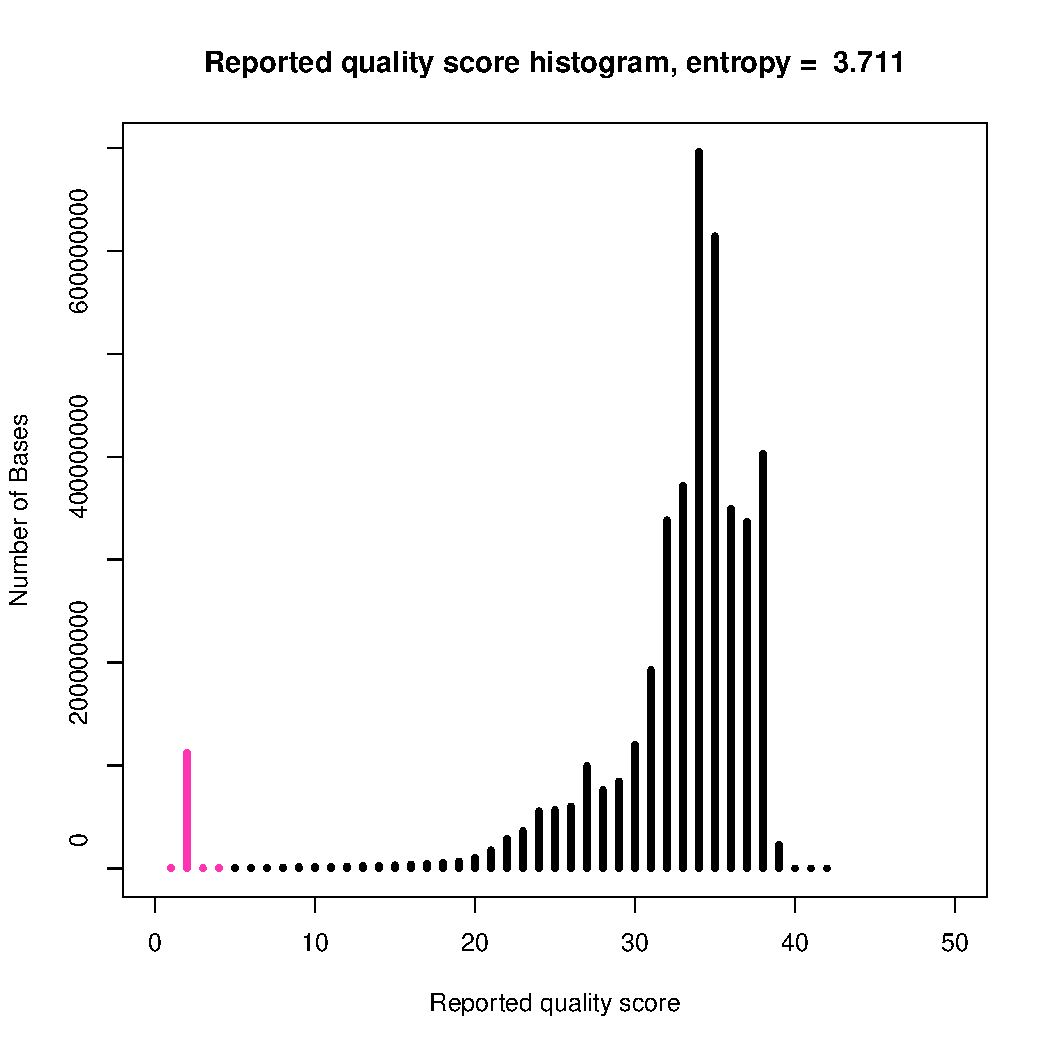
\includegraphics[width=0.9\linewidth]{alinhamento_rms/exome.sorted.dedup.real.fixed.recal.stats.after/quality_rep_hist.pdf}}
  \caption{Depois da recalibração do escore de qualidade}
\end{subfigure}
\caption[Número de Bases vs Escore de Qualidade]{Nessa figura podemos observar uma distribuição maior do valor médio do escore de qualidade.}
\label{fig:rms_quality_rep_hist}
\end{figure}

\begin{figure}
\centering
\Large\textbf{Qualidade (Empírico - Reportado) vs Dinucleotídeos}\par\medskip
\begin{subfigure}{.7\textwidth}
  \centering
  \fbox{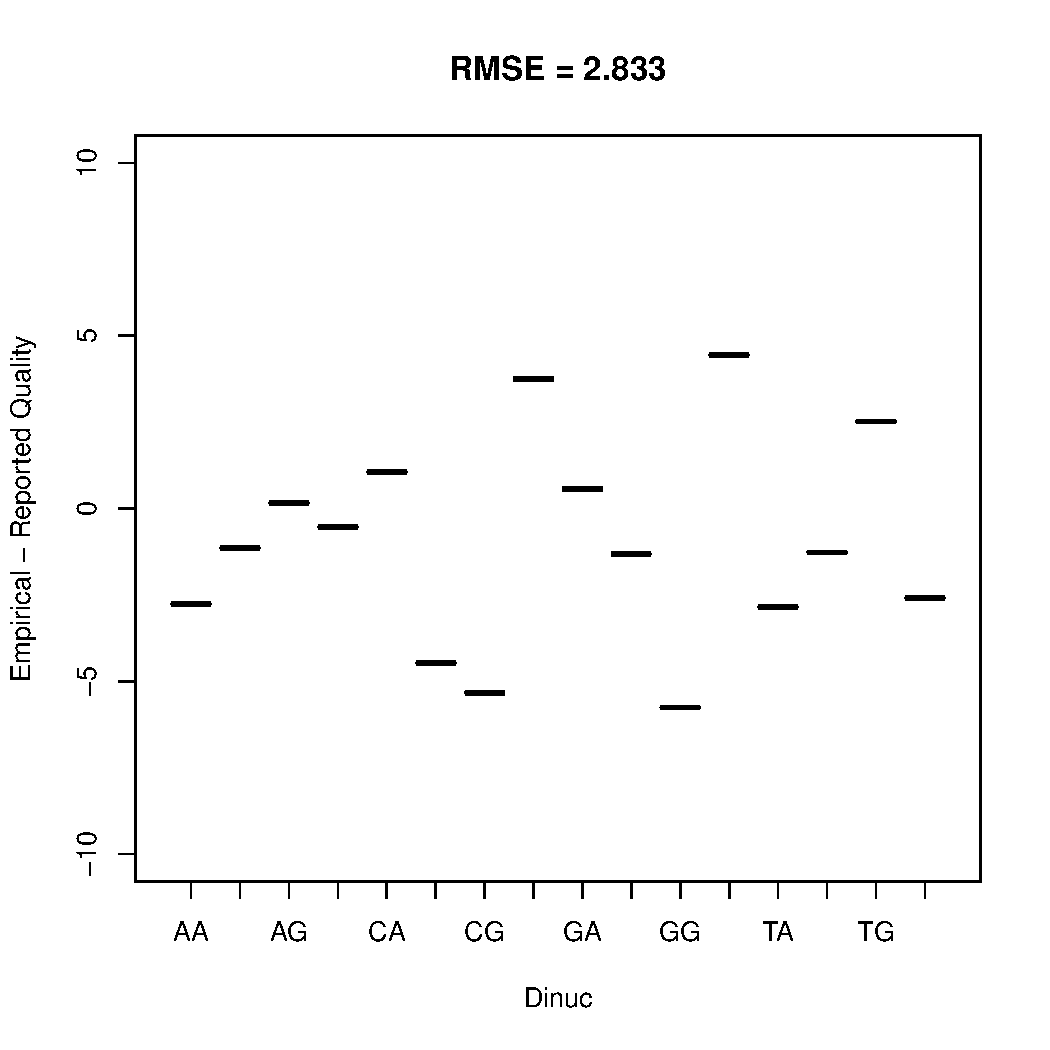
\includegraphics[width=0.9\linewidth]{alinhamento_rms/exome.sorted.dedup.real.fixed.recal.stats.before/qual_diff_v_Dinuc.pdf}}
  \caption{Antes da recalibração do escore de qualidade}
\end{subfigure}%
\begin{subfigure}{.7\textwidth}
  \centering
  \fbox{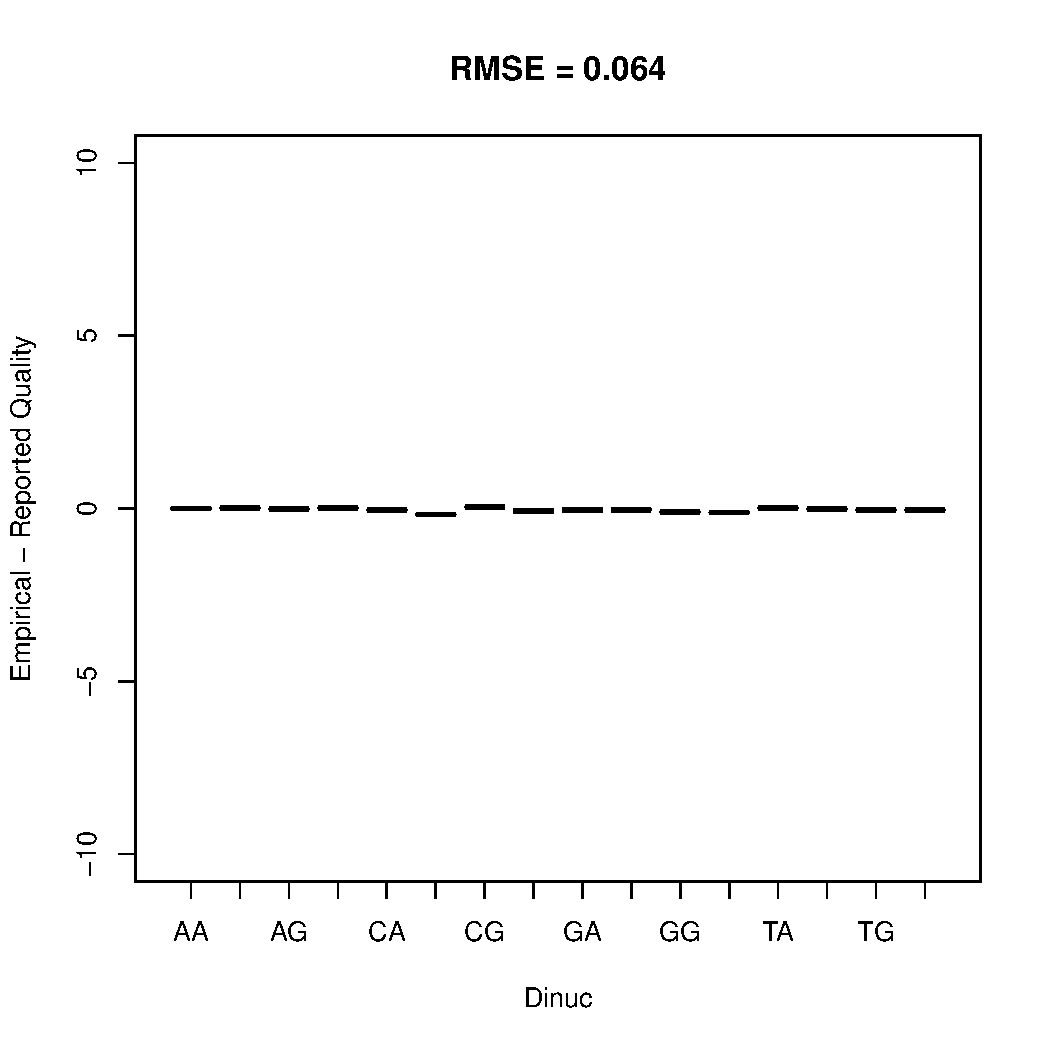
\includegraphics[width=0.9\linewidth]{alinhamento_rms/exome.sorted.dedup.real.fixed.recal.stats.after/qual_diff_v_Dinuc.pdf}}
  \caption{Depois da recalibração do escore de qualidade}
\end{subfigure}
\caption[Qualidade (Empírico - Reportado) vs Dinucleotídeos]{Nesta figura podemos observar uma correção da qualidade para cada dinucleotídeo.}
\label{fig:rms_qual_diff_v_Dinuc}
\end{figure}

\end{landscape}

}


Na figura \ref{fig:rms_before_emp_v_stated} apresentamos o antes e o depois para os valores de qualidade empíricos contra os valores reais estimados. Podemos notar que este método realiza uma normalização dos dados de maneira a corrigir um viés existente por causa das particularidades de cada tecnologia de sequenciamento.

Na figura \ref{fig:rms_quality_rep_hist} apresentamos a relação entre o número de bases e os valores de qualidade em phred escore. Neste gráfico podemos observar que a maior parte das bases estão com um phred escore entre 30 e 40 o que pode ser considerado um resultado muito bom.

Na figura \ref{fig:rms_qual_diff_v_Dinuc} podemos notar um viés da relação entre a qualidade empírica e reportada para diferentes tipos de dinucleotídeos. Neste processo os valores são normalizados ao redor de 0, para ajudar a reduzir o número de falsos positivos no processo seguinte de calling de variantes.

\subsubsection{Chamada de variantes}

O processo de chamada ``\textit{calling}'' de variantes foi realizado com o método UnifiedGenotyper do GATK considerado o padrão ouro atualmente para se fazer esse tipo de tarefa.

A tabela \ref{rms_calling} apresenta um resumo dos resultados obtidos neste processo:

\afterpage{
\begin{landscape}

\begin{table}[p]
\caption{Resultado do processo de calling de variantes realizado usando o método UnifiedGenotyper para o indivíduo RMS}
\begin{center}
\scalebox{1.5}{
\begin{tabular}{|r|l|}
\hline
Bases visitadas & 47.195.691 \\ \hline
Bases que podem ser chamadas & 46.982.901 \\ \hline
Bases chamadas com confiança & 827.992 \\ \hline
\% de bases que podem ser chamadas de todas as regiões & 99,549 \\ \hline
\% de bases que podem ser chamadas com confiança de todas as regiões & 1,754 \\ \hline
\% de bases chamadas com confiança de todas as regiões & 1,762 \\ \hline
Chamadas realmente feitas (variantes realmente encontradas) & 39.677 \\ \hline
\end{tabular}
}
\end{center}
\label{rms_calling}
\end{table}
\end{landscape}

\clearpage
}

Podemos observar que tivemos um \textit{calling} de 39.677 variantes em 47.195.691 bases visitadas no total, o que corresponde a 1.75\% do genoma. De todas as bases cobertas 827.992 puderam ser genotipadas com um grau de confiança de 99.5\%. A cobertura média desse exoma foi de 29.96X e o valor do escore de qualidade médio foi de 504.62.

\subsubsection{Recalibração do Escore de Qualidade da Variante}

Neste processo nós utilizamos um conjunto de dados com genótipos dos indivíduos do projeto HapMap 3 que foram validados utilizando arrays de SNPs e com isso criamos um modelo de treinamento sobre esses atributos. Este modelo é então aplicado no arquivo VCF para melhorar a qualidade das variantes obtidas e ajudar a reduzir o número de falsos positivos.

\subsubsection{Processo de Filtragem de Indels}

Este processo consiste na aplicação de alguns critérios de filtragem para eliminar indels de baixa qualidade, como por exemplo: 

\begin{itemize}
 \item QD < 2.0
 \item ReadPosRankSum < -20.0
 \item InbreedingCoeff < -0.8
 \item FS > 200.0 
\end{itemize}

Esses valores foram obtidos a partir do site do GATK em seu documento sobre ``\textit{Best Practices for Variant Detection}''

Site: \url{https://www.broadinstitute.org/gatk/guide/best-practices}

\section{Anotação de Exomas}

Após a obtenção do arquivo VCF final gerado pelo programa GATK, um script em python realiza a anotação dos dados utilizando os programas SNPEFF, Variant Annotator (GATK) e o Annovar integrando os resultados de cada um dos programas em um único arquivo VCF final. Após obtermos os resultados da anotação surgiu a ideia de construir uma ferramenta online que permitisse a filtragem das variantes por médicos e cientistas, de maneira que esta operação pudesse ser realizada através de uma interface web que permitisse a identificação de variantes que pudessem estar associadas com a doença.

\section{Mendel,MD - Construção da Ferramenta}

A seguir apresentamos o software Mendel,MD, que foi desenvolvido para investigação dos casos clínicos recebidos pelo Laboratório de Genômica Clínica da Faculdade de Medicina da UFMG. Esse programa foi criado para permitir o armazenamento, a anotação e a filtragem de variantes dos pacientes que foram estudados pelo nosso grupo, com a ideia de criar uma maneira fácil de atualizar os dados rapidamente, toda vez que novos conjuntos de dados, programas ou métodos fossem disponibilizados, de forma simples e modular, facilitando ao máximo a repetição das tarefas que fossem comuns. Este \textit{pipeline} pode ser facilmente adaptado ou modificado para inclusão de novos métodos e novas ferramentas.

\subsection{Banco de Dados}
A modelagem do banco de dados foi feita através de um arquivo chamado \textit{models.py} que possui classes em python que descrevem os campos que devem ser armazenados em cada uma das tabela do banco de dados. Após a criação deste arquivo, o Django passa então a controlar os processos de criação e atualização desses campos. Além disso ele também fica responsável pela busca e remoção dos dados através uma técnica conhecida como Mapeamento de Objetos Relacionais (ORM) que facilita a criação de consultas em Python que são transformadas em SQL para se realizar consultas ao banco de dados. Isso é muito utilizado para filtrar as variantes de cada paciente de acordo com os parâmetros que forem escolhidos pelo médico ou pesquisador que estiver utilizando o Mendel,MD.

No anexo~\ref{lst:modelo_individuo} apresentamos o modelo que foi desenvolvido para armazenar as informações sobre cada individuo. Neste arquivo ficam armazenadas informações como por exemplo o nome de usuário que fez o upload do arquivo VCF, a data do upload, o nome completo do arquivo e algumas informações sobre o estado do arquivo dentro do sistema.

Após ser inserido no Mendel,MD, o arquivo VCF passa a ter três estados possíveis dentro do sistema: \textit{new}, \textit{annotated} e \textit{populated}. O estado \textit{new} indica que o arquivo acabou de ser enviado ao sistema e está na fila para ser anotado pelo nosso programa, o estado \textit{annotated} significa que ele passou por todo o \textit{pipeline} de anotação com sucesso e está pronto na fila para ser inserido no banco de dados e o estado \textit{populated} indica que ele já foi inserido no banco de dados com sucesso e está pronto para ser analisado pelo usuário final.

No anexo~\ref{lst:modelo_variantes} apresentamos o modelo que foi desenvolvido para armazenar as informações sobre as variantes de cada indivíduo. Podemos observar que além dos campos já presentes no VCF, foram criados alguns campos para ajudar na filtragem de variantes como por exemplo a frequência da variante em relação a diferentes bancos de dados (ex. 1000genomesn, dbSNP e ESP6500) e alguns escores de patogenicidade como por exemplo SIFT e Polyphen-2 e CADD. Também podemos observar que alguns campos foram criados para armazenar as informações de duas ferramentas que foram integradas no sistema SnpEff e VEP.

Para recuperarmos a partir do banco todas as variantes do primeiro indivíduo do nosso banco de dados usamos o seguinte código em Python (Django):

\begin{verbatim}
Variants.objects.all(individual_id=1)
\end{verbatim}

Se quisermos obter todas as variantes desse indivíduo que são homozigóticas nós usamos o seguinte código:

\begin{verbatim}
Variants.objects.all(individual_id=1, variant_type="HOM")
\end{verbatim}

Essa codificação dos campos em Python permite que eles sejam facilmente traduzidos para um código SQL compatível com o sistema gerenciador de banco de dados (SGBD) que estiver sendo utilizado pelo projeto, que no nosso caso é o banco PostgreSQL.

Os dados deste trabalho foram inicialmente armazenados em um banco MySQL e posteriormente migrados para um banco PostgreSQL. Isso aconteceu porque o número de registros armazenados na tabela de variantes ultrapassou 10 milhões e a consulta ao banco de dados começou a ficar muito lenta, por exemplo, quando muitos indivíduos fossem utilizados como controles durante o processo de análise e filtragem de variantes. Após a migração do banco nós obtivemos um aumento de desempenho considerável que ajudou a melhorar bastante a usabilidade do sistema.

Na tabela \ref{table:registros} nós apresentamos informações sobre o número de registros armazenados em cada uma das tabelas do banco de dados. Aqui é possível visualizar o número de indivíduos, genes, doenças e vias metabólicas que foram armazenados em cada uma das tabelas do banco. Esses dados são muito importantes para auxiliarem na filtragem de variantes de cada indivíduo.



\afterpage{
\begin{table}[p]
\caption{Informação sobre o número de registros armazenados em cada uma tabelas do sistema.}
\begin{center}
\scalebox{0.65}{
\begin{tabular}{|p{6cm}|p{2cm}|p{10cm}|p{3cm}|}
\hline
\textbf{Tabela} & \textbf{número de registros} & \textbf{Tabela} & \textbf{número de registros} \\ \hline
account\_emailaddress         & 8                  & djkombu\_queue                                & 3                  \\ \hline
account\_emailconfirmation    & 8                  & filter\_analysis\_familyfilteranalysis        & 0                  \\ \hline
auth\_group                   & 0                  & filter\_analysis\_filteranalysis              & 0                  \\ \hline
auth\_group\_permissions      & 0                  & filter\_analysis\_filterconfig                & 0                  \\ \hline
auth\_permission              & 150                & genes\_cgdcondition                           & 3.607               \\ \hline
auth\_user                    & 12                 & genes\_cgdentry                               & 2.725               \\ \hline
auth\_user\_groups            & 0                  & genes\_cgdentry\_CONDITIONS                   & 3.958               \\ \hline
auth\_user\_user\_permissions & 0                  & genes\_cgdentry\_INTERVENTION\_CATEGORIES     & 3.635               \\ \hline
cases\_case                   & 0                  & genes\_cgdentry\_MANIFESTATION\_CATEGORIES    & 7.319               \\ \hline
cases\_case\_case\_groups     & 0                  & \textbf{genes\_gene}                          & \textbf{37.215}     \\ \hline
cases\_case\_cases            & 0                  & genes\_gene\_diseases                         & 5.725               \\ \hline
cases\_case\_children         & 0                  & genes\_genecategory                           & 0                  \\ \hline
cases\_case\_control\_groups  & 0                  & genes\_genecategory\_genes                    & 0                  \\ \hline
cases\_case\_controls         & 0                  & genes\_genegroup                              & 0                  \\ \hline
cases\_case\_shared\_with     & 0                  & genes\_genelist                               & 62                 \\ \hline
celery\_taskmeta              & 712                & genes\_goterm                                 & 0                  \\ \hline
celery\_tasksetmeta           & 0                  & genes\_goterm\_children                       & 0                  \\ \hline
databases\_varisnp            & 78.951 & genes\_goterm\_parents                        & 0                  \\ \hline
\textbf{diseases\_disease}    & \textbf{6.845}     & genes\_intervention                           & 20                 \\ \hline
diseases\_gene                & 4.715              & genes\_manifestation                          & 19                 \\ \hline
diseases\_gene\_diseases      & 6.845              & genes\_membership                             & 0                  \\ \hline
diseases\_hgmdgene            & 0                  & individuals\_controlgroup                     & 0                  \\ \hline
diseases\_hgmdgene\_diseases  & 0                  & individuals\_controlvariant                   & 0                  \\ \hline
diseases\_hgmdmutation        & 0                  & individuals\_group                            & 3                  \\ \hline
diseases\_hgmdphenotype       & 0                  & individuals\_group\_members                   & 76                 \\ \hline
django\_admin\_log            & 2                  & \textbf{individuals\_individual}              & \textbf{221}       \\ \hline
django\_content\_type         & 50                 & individuals\_individual\_shared\_with\_groups & 179                \\ \hline
django\_select2\_keymap       & 0                  & individuals\_individual\_shared\_with\_users  & 0                  \\ \hline
django\_session               & 511                & individuals\_usergroup                        & 1                  \\ \hline
django\_site                  & 1                  & individuals\_usergroup\_members               & 2                  \\ \hline
djcelery\_crontabschedule     & 0                  & pathway\_analysis\_pathway                    & 289                \\ \hline
djcelery\_intervalschedule    & 0                  & socialaccount\_socialaccount                  & 0                  \\ \hline
djcelery\_periodictask        & 0                  & socialaccount\_socialapp                      & 0                  \\ \hline
djcelery\_periodictasks       & 0                  & socialaccount\_socialapp\_sites               & 0                  \\ \hline
djcelery\_taskstate           & 0                  & socialaccount\_socialtoken                    & 0                  \\ \hline
djcelery\_workerstate         & 0                  & \textbf{variants\_variant}                    & \textbf{25.304.952}  \\ \hline
djkombu\_message              & 0                  &                                               &                    \\ \hline
\end{tabular}
}
\end{center}
\label{table:registros}
\end{table}
\clearpage
}

\normalsize

Atualmente o nosso banco de dados possui 221 exomas e isso equivale a 25.304.952 variantes.

\subsection{Dashboard}

Para facilitar a visualização dos indivíduos no sistema foi desenvolvida uma interface chamada de \textit{Dashboard} que exibe uma lista com todos os arquivos que foram enviados para o sistema. Na figura \ref{fig:dashboard} apresentamos essa interface e podemos observar que com ela é possível verificar diversas informações sobre cada indivíduo como o nome de cada arquivo, o número de variantes, a data de envio, o estado atual do arquivo no sistema entre outras informações. Também nesta página é possível realizar operações em massa como por exemplo, selecionar múltiplos indivíduos através de uma caixa de seleção ao lado de cada indivíduo pra poder enviar os arquivos para serem re-anotados ou re-inseridos no banco de dados sempre quando for necessário. Este tipo de interface facilita muito a manipulação e anotação dos VCFs sempre que houver novas informações para serem integradas na análise de exomas.


\afterpage{
\begin{landscape}
\begin{figure}[p]
  \centering
    \Large\textbf{Dashboard - Interface para visualização dos indivíduos no sistema}\par\medskip
  \fbox{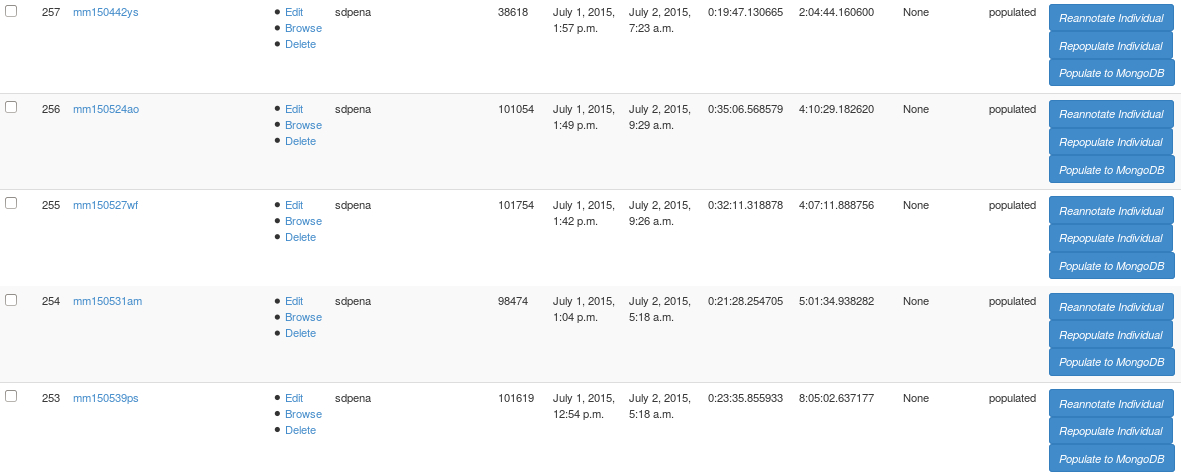
\includegraphics[width=1.3\textwidth]{./Figures/mendelmd/Dashboard.png}}
  \caption[Dashboard - Interface para visualização dos indivíduos no sistema]{A partir desta interface é possível visualizar as variantes de cada indivíduo, reanotar os indivíduos e reinserí-los no banco de dados. Da esquerda para a direita temos as colunas: ID, nome da amostra, usuário, número de variantes, Data da criação, data da modificação, tempo de anotação, tempo de inserção no banco de dados e estado da amostra.}
  \label{fig:dashboard}
\end{figure}
\end{landscape}

\clearpage
}


\subsection{Upload de Genomas}

A figura~\ref{fig:upload} apresenta a interface de submissão de indivíduos para o sistema. Essa interface foi desenvolvida utilizando a biblioteca de javascript chamada Jquery FileUpload e facilita o envio de arquivos VCFs para o sistema permitindo o upload simultâneo de indivíduos para o servidor usando para isso qualquer dispositivo (computador, tablet ou celular) que tenha acesso a internet.

\afterpage{
  \begin{landscape}
\begin{figure}[p]
  \centering
  \Large\textbf{Interface para submissão dos indivíduos no sistema}\par\medskip
  \fbox{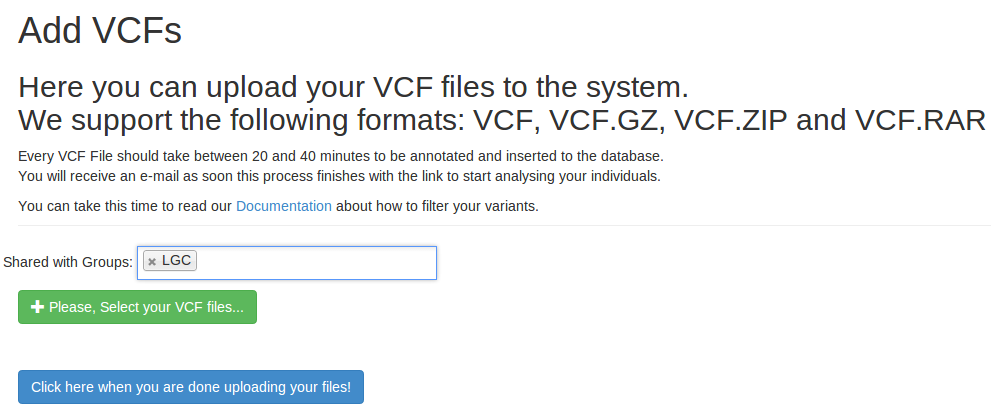
\includegraphics[width=1.5\textwidth]{./Figures/mendelmd/upload.png}}
  \caption[Interface para submissão dos indivíduos no sistema]{A interface de submissão dos indivíduos foi desenvolvida utilizando a biblioteca Jquery FileUpload para facilitar essa tarefa.}
  \label{fig:upload}
\end{figure}
\end{landscape}
\clearpage
}


\subsection{Agendador de Tarefas}

O Celery é um sistema agendador de tarefas assíncronas e distribuídas que permite a integração e execução de diferentes scripts e programas. Este programa foi utilizado para permitir a anotação automática dos dados de maneira totalmente assíncrona a partir do momento que o usuário realiza o upload dos dados no sistema. Nas figuras~\ref{fig:celery_shell} e~\ref{fig:celery_annotation} apresentamos a interface do celery, na figura ~\ref{fig:celery_annotation} é possível verificar diversos scripts sendo executados em paralelo para realizar a anotação de um exoma que foi inserido no sistema.

\afterpage{
  \begin{landscape}
\begin{figure}[p]
  \centering
  \Large\textbf{Interface do Celery}\par\medskip
    \fbox{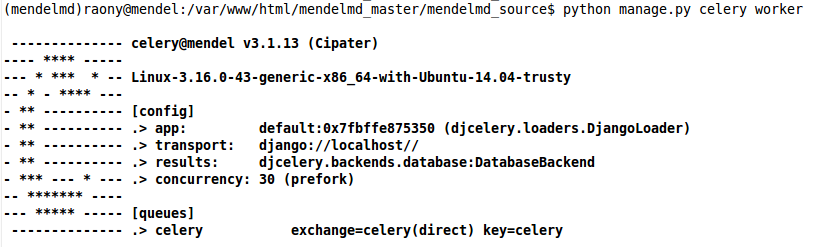
\includegraphics[width=1.5\textwidth]{./Figures/Celery_Shell.png}}
  \caption[Interface do Celery]{Nesta figura podemos visualizar a interface de comando do Celery. Nesta interface podemos verificar o output de cada programa utilizado durante a anotação de variantes.}
  \label{fig:celery_shell}
  \end{figure}
\end{landscape}

\clearpage
}


\afterpage{
  \begin{landscape}
\begin{figure}[p]
  \centering
  \Large\textbf{Processo de anotação de variantes}\par\medskip
  \fbox{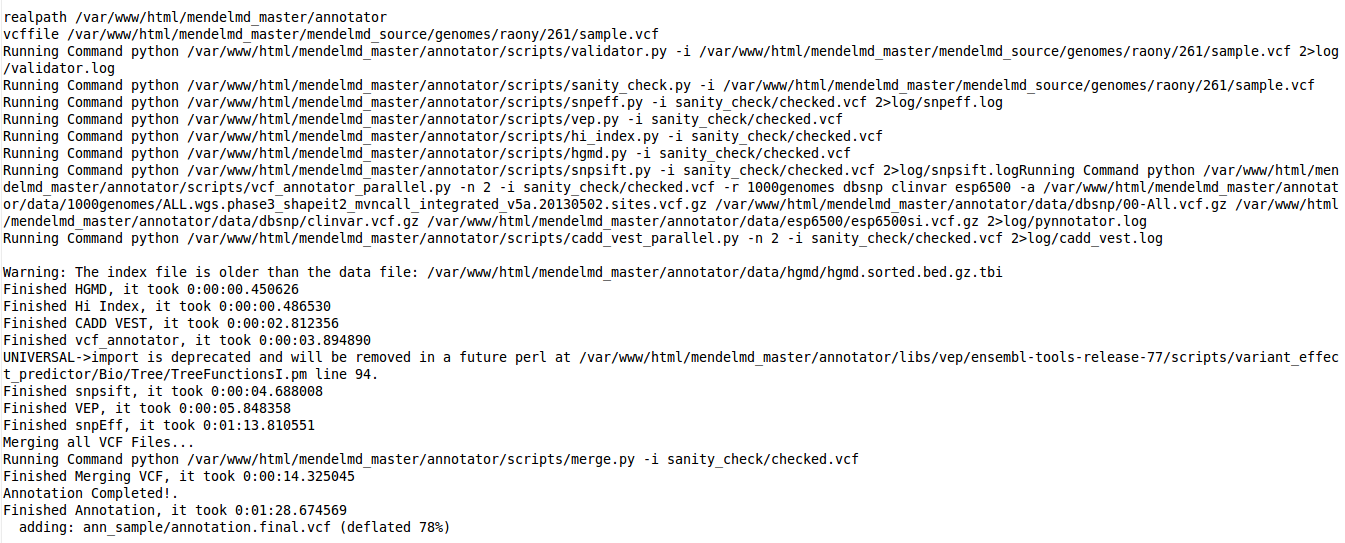
\includegraphics[width=1.5\textwidth]{./Figures/Celery_annotation.png}}
  \caption[Processo de anotação de variantes]{Nesta figura podemos observar diversos scripts sendo executados em paralelo utilizando o Celery para realizar a anotação de exomas através do uso de diferentes programas como SnpEff e VEP.}
  \label{fig:celery_annotation}
  \end{figure}
\end{landscape}

  
  \clearpage
}

\subsection{Conversão dos dados para CSV}

Apesar do Mendel,MD ter sido criado para facilitar o processo de filtragem dos dados utilizando para isso uma interface web, nós também desenvolvemos um script em python para realizar a conversão dos dados de VCF para CSV após o término do processo de anotação. Além disso foi desenvolvido uma programa usando wxPython que permite a conversão entre arquivos do tipo VCF para CSV de maneira local utilizando para isso uma interface gráfica com janelas e botões. Isso permite que o usuário converta os dados de VCF para CSV para que eles possam ser filtrados manualmente pelo Médico ou Pesquisador usando um programa de planilhas, como por exemplo o Excel ou o Libre Office Calc.

A figura~\ref{fig:vcf2csv} apresenta a interface gráfica desenvolvida para realizar essa conversão entre os formatos VCF e CSV. Essa transformação entre os formatos também realiza a de-normalização dos dados presentes nas colunas INFO do VCF de maneira que todos os dados dessa coluna fiquem separados em colunas diferentes no arquivo CSV final.

Além disso, também foi adicionada uma opção para que o usuário pudesse alterar a ordem das colunas no arquivo de saída.

\afterpage{
\begin{landscape}

\begin{figure}[p]
  \centering
  \Large\textbf{Programa desenvolvido para conversão entre arquivos VCF e CSV}\par\medskip
  \fbox{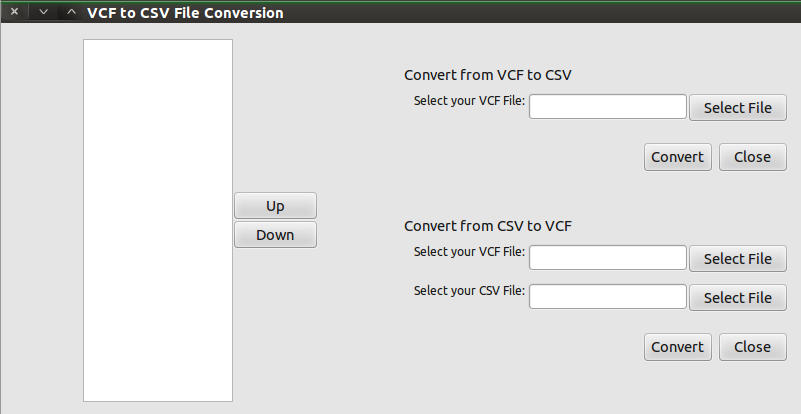
\includegraphics[width=1.5\textwidth]{./Figures/vcf2csv.png}}
  \caption[Programa desenvolvido para conversão entre arquivos VCF e CSV]{Interface do programa desenvolvido para conversão entre os formatos VCF e CSV.}
  \label{fig:vcf2csv}
\end{figure}
\end{landscape}
\clearpage
}

\subsection{Anotação de Variantes}

Para realizar a integração de diferentes ferramentas e fontes de informação, foi desenvolvido um \textit{framework} que realiza toda a anotação das variantes e que integra a maior parte dos dados e ferramentas existentes relacionados a este tipo de análise. A figura \ref{fig:framework_anotacao} é a principal figura deste trabalho, onde é apresentado o \textit{framework} que foi desenvolvido durante este trabalho. Pode-se observar nesta figura todos os processos que ocorrem dentro do pipeline de anotação desenvolvido para o Mendel,MD.

Após a inserção dos indivíduos no sistema, nós primeiramente realizamos uma validação dos arquivos VCFs através de um método chamado ``\textit{vcf-validator}'' que faz parte do programa \textit{VCFTools}. Este método realiza diversos testes no arquivo VCF de entrada e ao final gera um arquivo com todos os problemas que foram encontrados. Após essa validação inicial o arquivo passa então por um método que desenvolvemos chamado de ``\textit{sanity-check}'' que prepara o arquivo VCF para ser anotado por diferentes ferramentas.

Uma das primeiras ferramentas integradas para a anotação dos dados foi o SNPEFF que entre outras coisas fornece informações importantes sobre cada mutação como por exemplo a classificação do seu impacto de acordo com as seguintes classes: MODIFIER, LOW, MODERATE e HIGH. Essas classes são extremamente úteis na hora de realizarmos a filtragem de variantes, o mais recomendado aqui seria primeiro fazer a busca em variantes que são MODERATE e HIGH pois aí estarão presentes as mutações que são mais graves e possivelmente podem causar uma alteração da estrutura de uma proteína.

Outro programa integrado pela nossa anotação foi o Variant Effect Predictor (VEP). Este programa realiza a anotação das variantes em relação aos tipos de mutações encontradas, aos aminoácidos que estão alterados, e caso ela seja uma mutação não-sinônima, anota a posição em relação ao cDNA. Além disso, o VEP também fornece escores de patogenicidade como por exemplo o SIFT e o Polyphen2 que são os escores mais utilizados atualmente quando buscamos por variantes patogênicas.

O banco de dados dbNFSP trouxe a capacidade de agregar centenas de informações diferentes para nossa análise como por exemplo anotação em relação a diferentes bancos de dados, escores de patogenicidade e de conservação de mutações. Para integrar essa ferramenta nós desenvolvemos um script em python chamado de ``\textit{pynnotator}'' que por sua vez utiliza bibliotecas como \textit{pysam} e \textit{parallel python} para realizar a anotação dos dados de uma maneira rápida eficiente, inclusive fazendo o uso de  múltiplos cores do processador ao mesmo tempo. Esse tipo de implementação não foi trivial mas ajudou bastante a diminuir o tempo necessário para se realizar a anotação de cada VCF contra uma grande quantidade de dados. O tempo médio de anotação para cada exoma enviado para o sistema é de apenas dez minutos.

\afterpage{
\begin{landscape}

\begin{figure}[p]
  \centering
  \Large\textbf{Framework de anotação de variantes}\par\medskip
 \fbox{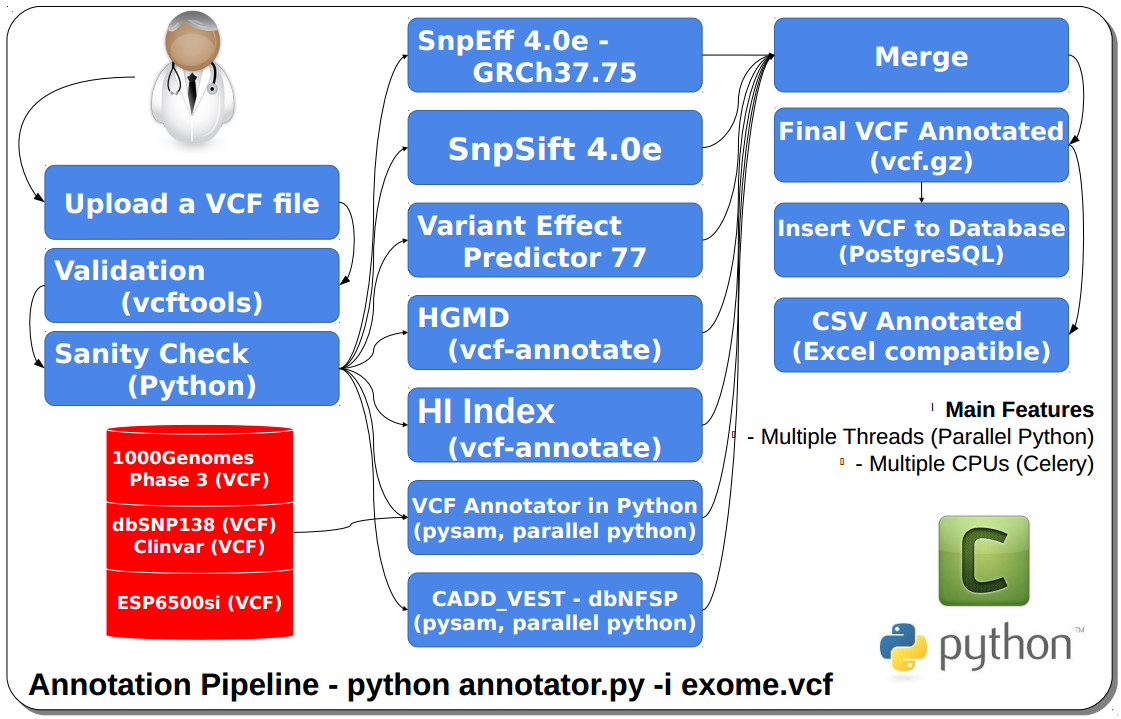
\includegraphics[width=1.2\textwidth]{./Figures/mendelmd/annotation_pipeline.png}}
 \caption[Framework de anotação de variantes]{Este foi o framework de anotação de variantes desenvolvido durante este trabalho, ele realiza a integração de diversas ferramentas e bancos de dados diferentes através de scripts desenvolvidos em python para automatizar todo o processo.}
 \label{fig:framework_anotacao}
\end{figure}
\end{landscape}

\clearpage
}

\subsection{Controle de Qualidade sobre os dados}

Para se realizar o controle de qualidade sobre os dados foi desenvolvida uma interface para calcular e mostrar métricas de qualidade calculadas a partir dos VCFs de cada indivíduo. Na figura \ref{fig:individuals_view} podemos observar algumas o número de variantes homozigotas e heterozigotas (0/1 e 1/1). Além disso nesta seção é possivel verificar outras métricas como o número de variantes para cada indivíduo, a cobertura média de cada exoma, a qualidade média de suas variantes, o número de variantes por cromossomo, o número de variantes por classe funcional entre outras opções que são apresentadas.

\afterpage{
    \begin{landscape}
\begin{figure}[p]
  \centering
    \Large\textbf{Interface para visualizar métricas sobre os dados inseridos}\par\medskip
   \fbox{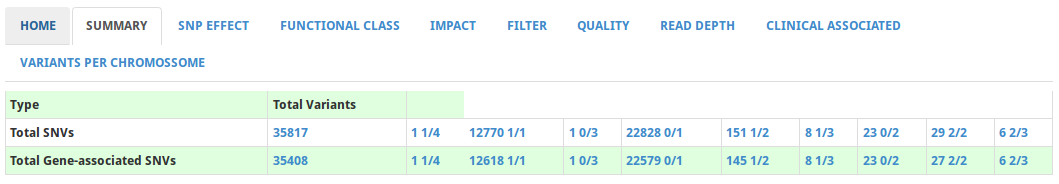
\includegraphics[width=1.5\textwidth]{./Figures/mendelmd/individuals_view.png}}
  \caption[Interface para visualizar métricas sobre os dados inseridos]{Nesta interface podes visualizar o número total de variantes, os tipos de variante encontradas no indivíduo e diversas outras métricas que são importantes para auxiliarem na filtragem de variantes como o número médio de qualidade e de cobertura para cada indivíduo.}
  \label{fig:individuals_view}
    \end{figure}
\end{landscape}


\clearpage
}

\subsection{Genes}

Na figura \ref{fig:genes_search} apresentamos a interface desenvolvida para realizar a busca de genes no sistema. Com essa interface é possível buscar genes por ``gene symbol'', por exemplo ``\textit{SUCLA2}'' ou então por uma parte do nome do gene ``succinate'' e então selecionar os genes obtidos nos resultados para serem utilizados no método de filtragem de variantes.

\afterpage{
  \begin{landscape}
\begin{figure}[p]
  \centering
  \Large\textbf{Interface para Busca de Genes}\par\medskip
  \fbox{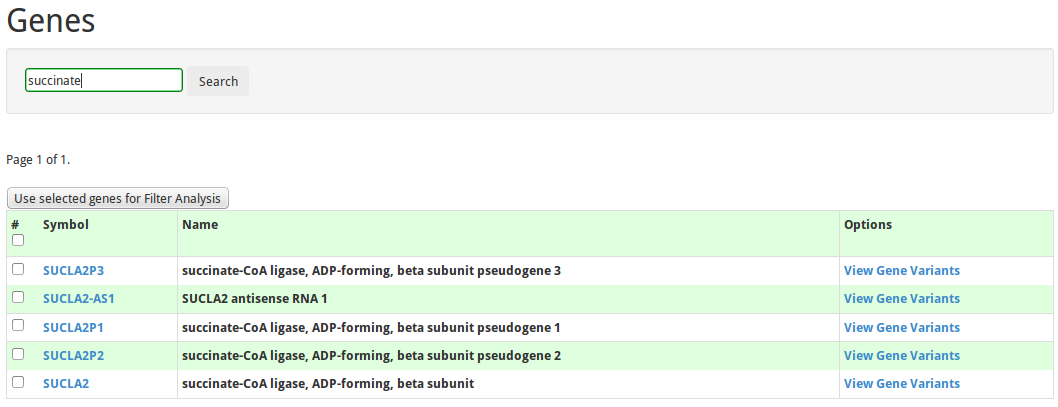
\includegraphics[width=1.5\textwidth]{./Figures/mendelmd/genes.png}}
  \caption[Interface para Busca de Genes]{Essa interface foi desenvolvida para permitir a busca de genes específicos, após a obtenção do resultado é possível investigar variantes apenas na lista de genes desejada.}
  \label{fig:genes_search}
  \end{figure}
\end{landscape}


  \clearpage
}

Também foi desenvolvida um opção para armazenar listas de genes personalizadas como por exemplo, com genes que já estivessem associados com doenças Mendelianas dominantes e recessivas. A figura \ref{fig:gene_lists} apresenta as listas de genes que foram inseridas no Mendel,MD.

\afterpage{
  \begin{landscape}
\begin{figure}[p]
  \centering
  \Large\textbf{Interface com grupos de genes adicionados}\par\medskip
  \fbox{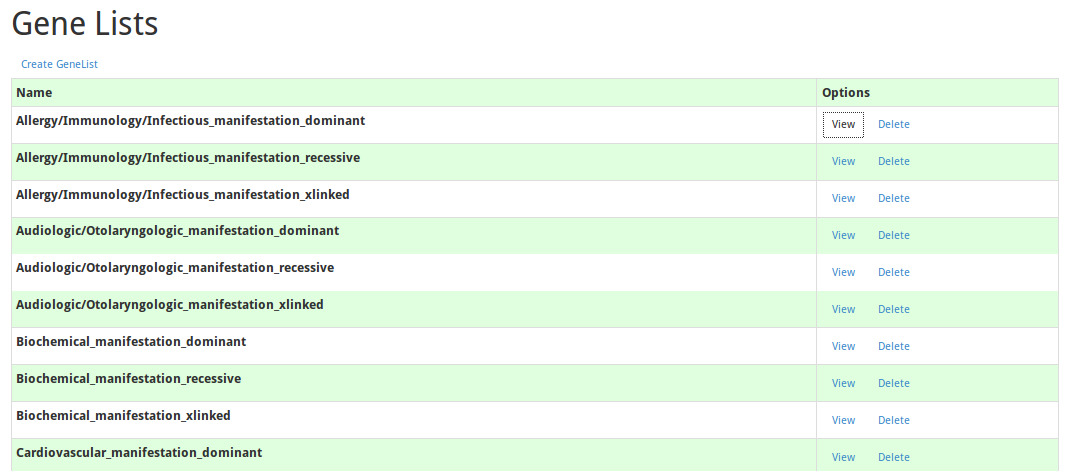
\includegraphics[width=1.5\textwidth]{./Figures/mendelmd/gene_lists.png}}
  \caption[Interface com grupos de genes adicionados]{Nesta interface podemos verificar os grupos de genes que foram criados pelos usuários de acordo com alguns critérios desejados.}
  \label{fig:gene_lists}
  \end{figure}
\end{landscape}

\clearpage
}

\subsection{Doenças}

Para obter dados sobre doenças Mendelianas nós utilizamos o site OMIM que possui atualmente 6845 doenças e 4715 genes. Esses dados foram inseridos no Mendel,MD para que fosse possível buscar por genes associados a doenças Mendelianas e para que eles pudessem ser inseridos no processo de filtragem de variantes.

Na figura \ref{fig:diseases} apresentamos a interface que permite a busca por doenças Mendelianas. Aqui é possível buscar por doenças e também selecionar os resultados para serem visualizados no método de filtragem de variantes na busca por variantes candidatas que estejam presentes nos indivíduos afetados pela doença. Nesta página o usuário pode digitar uma doença e selecionar todos os genes associados com ela para buscar variantes em seus indivíduos.

\afterpage{
  \begin{landscape}
\begin{figure}[p]
  \centering
  \Large\textbf{Interface para Busca de Doenças}\par\medskip
  \fbox{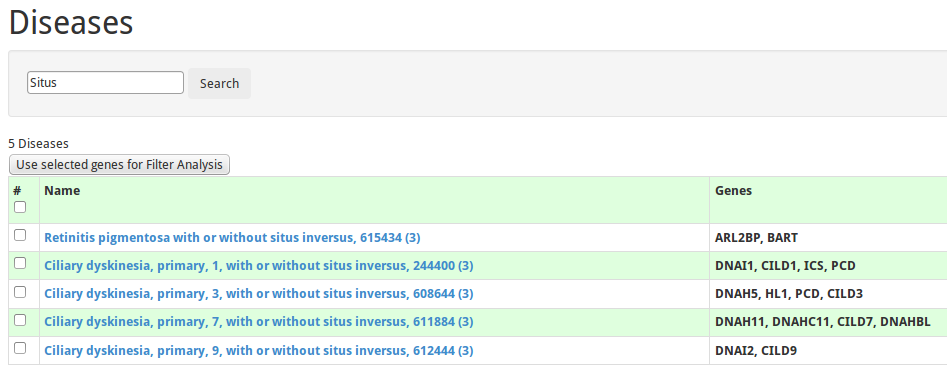
\includegraphics[width=1.5\textwidth]{./Figures/mendelmd/diseases.png}}
  \caption[Interface para Busca de Doenças]{Nesta interface podemos visualizar o resultado da busca por doenças com a palavra situs. A partir desta interface é possível visualizar variantes apenas em genes associados a um ou mais tipos específicos de uam determinada doença escolhida pelo usuário.}
  \label{fig:diseases}
  \end{figure}
\end{landscape}

\clearpage
}

\subsection{Filtragem de Variantes}

Após a anotação dos dados pelo sistema, o usuário pode filtrar as variantes dos indivíduos utilizando para essa tarefa um formulário web que permite a eliminação de variantes utilizando diferentes critérios de filtragem para tentar identificar a variante que possa ser responsável por causar a doença do paciente.

Este método foi implementado para permitir que essa tarefa pudesse ser repetida muitas vezes, facilitando a compreensão do que acontece durante cada etapa do processo e permitindo a combinação de diferentes opções de filtragem para chegar a uma lista pequena de candidatos.

As figuras a seguir ilustram o processo de filtragem implementado no Mendel,MD e que foram divididos em 3 etapas.
% 
% Step1Individuals.png
% Step2Variants.png
% Step3Databases.png
\afterpage{
  \begin{landscape}
\begin{figure}[p]
  \centering
    \Large\textbf{Filtragem de Variantes - 1ª Etapa}\par\medskip
    \fbox{\includegraphics[width=1.3\textwidth]{./Figures/Filtragem/Step1Individuals.png}}
  \caption[Filtragem de Variantes - 1ª Etapa]{Essa é a primeira tela da filtragem de variantes onde o usuário precisa selecionar as opções referentes aos indivíduos, genes e snps que deseja analisar.}
  \label{fig:filtering_step1}
  \end{figure}
\end{landscape}

\clearpage
}

A figura \ref{fig:filtering_step1} mostra a primeira etapa onde o usuário pode selecionar os indivíduos em que gostaria de visualizar as variantes existentes e também os indivíduos que gostaria que fossem utilizados como controles no processo de exclusão de variantes. Além disso o usuário pode utilizar uma lista de genes e SNPs que gostaria de incluir ou excluir nos indivíduos selecionados.

\afterpage{
  \begin{landscape}
\begin{figure}[p]
  \centering
    \Large\textbf{Filtragem de Variantes - 2ª Etapa}\par\medskip
    \fbox{\includegraphics[width=1.5\textwidth]{./Figures/Filtragem/Step2Variants.png}}
  \caption[Filtragem de Variantes - 2ª Etapa]{Nesta interface é possível selecionar algumas opções das variantes presentes nos arquivos VCF.}
  \label{fig:filtering_step2}
  \end{figure}
\end{landscape}

\clearpage
}


Na figura \ref{fig:filtering_step2} apresentamos a segunda etapa onde o usuário possui diversas opções para definir sobre o tipo de variante que gostaria de visualizar nos resultados. A primeira opção seria em relação ao tipo de variante homozigótica (Ex. 1/1, 2/2 e 3/3) ou heterozigótica (Ex. 0/1, 0/2 e 0/3), esses números correspondem ao genótipos que foram codificados no arquivo VCF para cada indivíduo. Existe uma opção que foi desenvolvida para selecionar apenas variantes em um único cromossomo ou então em uma região específica de um cromossomo como por exemplo: chr:17, pos:80789468-80789469. Isso pode ajudar na investigação de regiões homozigóticas onde possam existir variantes candidatas.

Nesta aba o usuário também pode selecionar o tipo da mutação, o cromossomo, a posição, a coluna de filtro do VCF (Ex. PASS, LowQual), o efeito da variante, a classe funcional, o impacto, o dbSNP Build de quando a variante foi inserida no dbSNP, a cobertura, a qualidade, o número de variantes por gene, exibir apenas variantes presentes em genes comuns entre os indivíduos selecionados, mostrar apenas variantes que não estejam presentes no dbSNP, mostrar apenas variantes anotadas como \textit{``clinically associated''} pelo clinvar e também excluir variantes presentes em regiões com segmento de duplicação


\afterpage{
  \begin{landscape}
\begin{figure}[p]
  \centering
    \Large\textbf{Filtragem de Variantes - 3ª Etapa}\par\medskip
    \fbox{\includegraphics[width=1.5\textwidth]{./Figures/Filtragem/Step3Databases.png}}
  \caption[Filtragem de Variantes - 3ª Etapa]{Nesta interface é possível selecionar valores em relação aos Bancos de Dados e Escores de Priorização que foram anotados para cada variante.}
  \label{fig:filtering_step3}
  \end{figure}
\end{landscape}

\clearpage
}

Conforme apresentado na figura \ref{fig:filtering_step3}, a terceira etapa permite a filtragem utilizando valores de máximo e mínimo da frequência possível das variantes em bancos de dados como 1000Genomes, dbSNP e ESP6500. Por último foram incluídos filtros para se eliminar variantes utilizando os escores de SIFT e Polyphen-2.

Além disso, também é possível utilizar outras opções como por exemplo, apenas genes relacionados a doenças específicas do OMIM. Ao começar a digitar, usamos uma função \textit{autocomplete} que foi desenvolvida usando uma biblioteca de Javascript chamada de Select2 que retorna uma lista de doenças para que o usuário possa adicionar em suas pesquisa. Isso facilita muito a investigação de doenças que possuam um fenótipo parecido mas que sejam causadas por genes diferentes. Rapidamente podemos adicionar diversos nomes de doenças na pesquisa que o sistema irá encontrar apenas os genes relacionados a estas doenças. 

\subsubsection{1-Click}

Nesta interface foi desenvolvida uma configuração padrão de filtros que são recomendados para o início do processo de filtragem de variantes. Esta interface foi desenvolvida para facilitar e automatizar a identificação de variantes causadoras de doenças Mendelianas.

O método 1-Click foi inspirado em uma opção da ferramenta de análise filogenética Phylogeny.fr e permite que o usuário selecione apenas os indivíduos da análise e o tipo de herança genética mais provável o que reduz drasticamente o número de variantes candidatas para tentar encontrar a real causadora da doença do indivíduo. Este método faz com que os filtros sejam configurados automaticamente para o usuário. Esses valores foram definidos de maneira empírica e são apenas uma sugestão sobre como realizar a configuração dos filtros.

As configurações pré-definidas estão listadas a seguir:

\begin{itemize}
  \item SnpEff Impact: HIGH ou MODERATE
  \item Profundidade de Leitura maior ou igual a 10
  \item Mostrar apenas variantes em genes comuns aos indivíduos selecionados
  \item Excluir Variantes presentes no banco VariSNP
  \item Frequência da variante no 1000Genomes menor que 0.005
  \item Frequência da variante no dbSNP137 menor que 0.005
  \item Frequência da variante no Exome Variant Server menor que 0.005
\end{itemize}

\subsubsection{Análise de Filtros para Famílias}

Este método permite a análise de famílias (Ex. Trios, Quartetos e etc) que podem ser utilizadas no processo de filtragem para encontrar variantes que sejam heterozigóticas nos pais dos indivíduos e que sejam homozigóticas nos filhos afetados. Isso também permite a identificação de variantes candidatas que tenham um padrão de herança chamado de heterozigoto composto, ou seja, quando o filho recebe um alelo do gene com defeito de cada um dos pais. Além disso esta opção também permite a visualização de variantes chamadas \textit{de novo}, ou seja, aquelas que estão presentes nos filhos mas que obrigatoriamente não estejam presentes em nenhum dos pais selecionados.

Para isso nós desenvolvemos uma interface onde é possível definir quem são os pais dos pacientes durante a análise. Então este método usa essa informação obtida para eliminar as variantes que estejam presentes nos pais e que não obedeçam aos critérios de herança estabelecidos. Na figura \ref{fig:family_analysis} podemos observar o formulário para este tipo de análise, e na figura \ref{fig:family_analysis_results} podemos verificar que nos resultados para cada genótipo encontrado nos filhos existe o genótipo de cada um dos pais. Quando selecionamos por exemplo a opção 'heterozigoto composto' o que acontece por trás é que o sistema mostra nos resultados apenas genes candidatos que possuem pelo menos uma variante de cada um dos pais. Esse tipo de análise ajuda muito a reduzir o número de genes candidatos.


\afterpage{
\begin{landscape}
\begin{figure}[p]
  \centering
    \Large\textbf{Interface do Family Analysis}\par\medskip
  \fbox{\includegraphics[width=1.5\textwidth]{./Figures/mendelmd/family_analysis.png}}
  \caption[Family Analysis]{Family Analysis - Neste formulário é possível selecionar quem são os pais dos indivíduos que estão sendo analisados para usar essa informação na hora da filtragem de dados}
  \label{fig:family_analysis}
\end{figure}
\clearpage
\end{landscape}
}




\afterpage{
\begin{landscape}
\begin{figure}[p]
  \centering
    \Large\textbf{Resultado do Family Analysis}\par\medskip
    \fbox{\includegraphics[width=1.5\textwidth]{./Figures/mendelmd/family_analysis_results.png}}
  \caption[Resultado do Family Analysis]{Nos resultados do Family Analysis é possível visualizar o genótipo de cada um dos pais para cada indivíduo nos resultados da análise}
  \label{fig:family_analysis_results}
\end{figure}
\end{landscape}

\clearpage
}
% 
% \subsubsection{Filter Pathway Analysis}
% 
% Este método mostra as variantes do resultado agrupadas por vias metabólicas do Kegg.  Isso permite a busca por variantes que estejam possivelmente associadas com uma única via metabólica. Para validar esta técnica utilizamos duas doenças chamadas Síndrome de \textit{Hurler} e de \textit{Hunter} que são causadas por mutações em genes diferentes (IDUA e IDS) mas que ambos os genes pertencem a via metabólica de glicosaminoglicanos. Na figura \ref{fig:pathway_analysis} podemos verificar que os resultados da análise estão agrupados por vias metabólicas. 
% 
% \afterpage{
% \begin{figure}[p]
%   \centering
%   \caption[Pathway Analysis]{Pathway Analysis - O resultado da filtragem aparece agrupado por vias metabólicas do KEGG}
%     \includegraphics[width=1.0\textwidth]{./Figures/mendelmd/pathway_analysis.png}
%   \label{fig:pathway_analysis}
% \end{figure}
% \clearpage
% }

\subsubsection{Visualização de variantes}

Ao encontrar uma variante de interesse é possível verificar todas as informações disponíveis sobre aquela variante no sistema clicando no botão ''View``. Para isso nós desenvolvemos uma interface que mostra todos os campos do banco de dados para aquela variante específica. Esta interface possui centenas de anotações para cada variante.

\subsubsection{Exportação de resultados}

Após o usuário realizar a filtragem dos dados do paciente é possível exportar as variantes restantes em formato csv clicando sobre o botão ''\textit{export to csv}`` para que elas possam ser investigadas manualmente por um clínico utilizando programas como por exemplo o Excel.

\subsection{Comparação de Exomas}

Para possibilitar a comparação de exomas de diferentes indivíduos e até mesmo de exomas do mesmo indivíduo gerados a partir de tecnologias diferentes foi desenvolvido um método de comparação de VCFs. O algoritmo implementado nesta comparação possui duas etapas: primeiro procura apenas por posições que sejam comuns aos dois indivíduos sendo comparados, depois verifica se o genótipo nessas posições é igual ou diferentes entre os dois arquivos.

Na figura \ref{fig:comparison} podemos observar a comparação do genótipo de dois irmãos (Exome\_2\_MB e Exome\_3\_EDS) através deste método. Nesta caso nós encontramos 48.110 variantes em posições em comum entre os dois irmãos sendo que 84.2\% dessas variantes tinham o mesmo genótipo nos dois indivíduos selecionados.

\afterpage{
\begin{landscape}
\begin{figure}[p]
  \centering
    \Large\textbf{Interface para comparação de indivíduos}\par\medskip
  \fbox{\includegraphics[width=1.3\textwidth]{./Figures/mendelmd/comparison.png}}
  \caption[Interface para comparação de indivíduos]{Essa interface foi desenvolvida para permitir a comparação de dois indivíduos ou VCFs.}
  \label{fig:comparison}
\end{figure}
\end{landscape}

\clearpage
}

%aqui termina construção mendel,md

\section{Casos Clínicos}

Nesta seção iremos discutir dois casos casos clínicos que foram recebidos para estudo pelo Laboratório de Genômica Clínica da Faculdade de Medicina da UFMG.

\subsection{Caso Clínico LGC 1}

O paciente RMS foi diagnosticado com duas doenças raras e pouco conhecidas \textit{situs inversus totalis} e panhipopituitarismo. 

\textit{Situs Inversus Totalis} é uma doença congênita onde todos os órgãos internos do indivíduo encontram-se invertidos, como exemplo, o coração encontra-se localizado no lado direito do peito ao invés do lado esquerdo. Este doença geralmente é acompanhada de problemas no trato respiratório, infertilidade, infecções no aparelho auditivo, e redução ou ausência de olfato. Estes problemas são causados por defeitos nos cílios e flagelos das células, sendo que um cílio é composto por um grupo de microtúbulos que são organizados em pares chamados de braços de dineína, recobertos por uma membrana chamada axonema. A ausência ou anormalidade dos braços de dineína conectando os nove pares de microtúbulos pode ser revelada através de uma microscopia eletrônica da célula. Apesar desta ser geralmente uma doença autossômica recessiva, ela também pode ser causada por mutações no cromossomo X \cite{Gebbia1997}.

Esta doença foi desenhada pela primeira vez por Leonardo da Vinci entre os períodos de 1452–1519, e foi reconhecida por Marco Aurélio Severino em 1643, porém, só foi descrita de uma maneira mais científica em 1793 por Matthew Baillie em seu livro "The Morbid Anatomy of Some of the Most Important Parts of the Human Body". Acredita-se que a incidência desta doença seja de 1 em cada 10.000 nascimentos. \cite{Report,Halasz2008}

Atualmente existem diversos genes associados com esta doença como por exemplo \textit{DNAI1, DNAH5, DNAH11, ZIC3 e CCDC11, IVS} \cite{Neesen2001,Olbrich2002, Bartoloni2002, Gebbia1997, Perles2012}.

Panhipopituitarismo é uma doença caracterizada pela ausência total ou parcial da glândula pituitária, o que provoca uma deficiência na produção de todos hormônios relacionados a este órgão. Este doença pode ser causada tanto por defeitos genéticos congênitos (presentes desde o nascimento) quanto por acidentes que danifiquem o hipotálamo ou a hipófise do indivíduo.

Entre os genes associados a esta doença podemos citar: \textit{HESX1, SOX2, SOX3, GLI2, LHX3, LHX4, PROP1, POU1F1} \cite{Viaroli2012}.

Um caso de panhipopituitarismo com situs inversus totalis foi descrito pela literatura em um paciente Húngaro de 56 anos\cite{Halasz2008}. Neste artigo o autor realizou o sequenciamento dos genes \textit{PIT1, PROP1, PITX2} a procura de mutações que pudessem estar relacionadas com a doença e no final eles concluíram não ter encontrado nenhuma mutação que pudesse ser responsável pelas doenças. Após a publicação deste artigo foi realizado o sequenciamento do exoma deste paciente e os dados foram compartilhados com nosso laboratório para análise junto com o exoma do nosso paciente RMS. A análise em conjunto desses dados não levou a nenhuma conclusão sobre uma mutação, ou gene, que pudesse ser compartilhado pelos dois indivíduos.

Além deste caso descrito pela literatura, outra paciente feminina de Boston, também foi diagnosticada com situs inversus totalis e panhipopituitarismo. Nós também recebemos os exomas dela e de sua família (pai, mãe e irmão) totalizando um quarteto de exomas que também foram analisados por nossa ferramenta a procura de mutações que pudessem ser compartilhadas entre os indivíduos afetados.

O tempo total de execução do pipeline completo para o indivíduo RMS foi de 12 horas.

Na tabela~\ref{rms_filtering_process} apresentamos o processo de filtragem de variantes sob um modelo recessivo que utilizado para o indivíduo RMS.

\afterpage{
\begin{table}[p]
\caption{Processo de Filtragem utilizado para o paciente RMS}
\begin{center}
\begin{tabular}{|p{9cm}|p{2.5cm}|p{2.5cm}|}
\hline
\textbf{Método de filtragem utilizado} & \textbf{Número de Variantes} & \textbf{Número de Genes} \\ \hline
Valores iniciais & 39.677 & 12.341 \\ \hline
Apenas variantes com o filtro PASS no VCF dos individuos. & 36.362 & 11.840 \\ \hline
Remoção de variantes encontradas em 292 exomas usados como controle. & 11.737 & 5.112 \\ \hline
Apenas variantes homozigóticas diferentes da referência Ex. 1/1, 2/1, 1/2. & 3.916 & 2.266 \\ \hline
Apenas variantes não sinônimas & 753 & 487 \\ \hline
Apenas variantes com um profundidade de leitura maior do que 10 (para uma cobertura média de 30X). & 644 & 428 \\ \hline
Apenas variantes em genes que possuem <=2 variantes por gene. & 434 & 386 \\ \hline
Remoção de variantes em regiões de segmento de duplicação. & 368 & 328 \\ \hline
Apenas variantes com frequência  menor do que 0.5\% nos indivíduos do 1000Genomes & 14 & 13 \\ \hline
Apenas variantes com frequência menor do que 0.5\% no dbSNP137 & 14 & 13 \\ \hline
Apenas variantes com frequência menor do que 0.5\% nos indivíduos do projeto ESP6500 & 8 & 8 \\ \hline
Apenas variantes com escore de SIFT entre 0  e 0.05 (Damaging) & 2 & 2 \\ \hline
Apenas variantes com escore de Polyphen-2 entre 0.85 e 1.0 (Damaging) & 1 & 1 \\ \hline
\end{tabular}
\end{center}
\label{rms_filtering_process}
\end{table}
\clearpage
}

Ao final da análise o gene restante \textit{GLRA4}, é um receptor de glicina alpha 4 e que não encontra-se associado a nenhuma das duas síndromes em estudo. Portanto, neste caso o mais recomendado seria aumentar o número de genes candidatos. A partir do momento que o número de genes obtidos estiver suficientemente pequeno, o usuário já pode investigar os genes um a um, para verificar se algum deles pode estar associado com a doença em estudo. 

Podemos observar que nenhum dos 13 genes candidatos (\textit{ZNF674}, \textit{C21orf62}, \textit{GPRIN2}, \textit{U52112.12}, \textit{OR52I1}, \textit{GLRA4}, \textit{VIL1}, \textit{DSPP}, \textit{HEPH}, \textit{TMEM199}, \textit{RP1L1}, \textit{SARM1}, \textit{PRR21}) pareceu estar associado com a doença, que nenhum deles foi descrito anteriormente como sendo o causador de nenhuma das duas doenças que foram diagnosticadas no indivíduo.

Apesar de todos os esforços não foi possível encontrar as causas destas doenças no paciente. Até mesmo a hipótese de que as variantes responsáveis possam estar em genes diferentes foi levantada devido a grande variedade de genes que poderiam ser responsáveis por causar ambas as doenças como por exemplo os genes \textit{OR52I1, GLRA4, VIL1 e DSPP}.

Este caso clínico foi importante para aprendermos a trabalhar com os dados de exomas e para automatizarmos o processo de análise para os futuros casos clínicos que seriam recebidos pelo nosso laboratório.

\subsection{Caso Clínico LGC 2}

Este caso clínico foi composto por 4 indivíduos de uma mesmo família, sendo dois irmãos (Exome\_3\_EDS e Exome\_4\_ELS) que haviam sido diagnosticados com síndrome de Leigh (OMIM:256000) e os seus pais (Exome\_5\_LS e Exome\_6\_DC) que não eram afetados pela doença.

A síndrome de Leigh possui 16 genes conhecidos no OMIM que podem conter variantes responsáveis por causar a doença, portanto este foi um caso ideal onde o sequenciamento e análise de exomas facilitou bastante o diagnóstico do paciente. 

A figura ~\ref{fig:sucla2} mostra os passos que foram utilizados para identificação da variante candidata no gene \textit{SUCLA2}.

Na figura \ref{fig:sucla2_view} nós apresentamos a visualização das variantes desta família em todos os cromossomos do genoma humano.

\afterpage{
\begin{figure}[p]
  \centering
    \Large\textbf{Processo de filtragem de variantes do caso LGC 2}\par\medskip
    \includegraphics[width=0.8\textwidth]{./Figures/SUCLA2_filtering_process.png}
  \caption[Processo de filtragem de variantes do caso LGC 2]{Nesta figura podemos observar o que aconteceu com o número de variantes e genes em cada etapa da filtragem para este caso clínico.}
  \label{fig:sucla2}
\end{figure}
\clearpage
}


\afterpage{
\begin{landscape}

\begin{figure}[p]
  \centering
    \Large\textbf{Visualização das variantes do caso LGC 2}\par\medskip
    \includegraphics[width=1.0\textwidth]{./Figures/case_lgc_2.png}
  \caption[Visualização das variantes do caso LGC 2]{Esta figura foi criada como uma representação as variantes para o caso LGC 2 - Os indivíduos Exome\_3\_EDS, Exome\_4\_ELS, Exome\_5\_LS e Exome\_6\_DC estão representados no sentido de dentro para fora da imagem.}
  \label{fig:sucla2_view}
\end{figure}
\end{landscape}
\clearpage
}


Nesta análise foram identificados 2 genes candidatos: \textit{SUCLA2} e \textit{OR5H2}. Uma pesquisa bibliográfica revelou um artigo publicado em 2007 \cite{Carrozzo2007} com mutações no gene \textit{SUCLA2} associadas com \textit{Leigh-Like Syndrome}(OMIM:612073).

Esse foi o primeiro caso clínico em que conseguimos identificar uma nova mutação, em um gene \textit{SUCLA2} (GENEID:8803) que já havia sido descrito pela literatura como associado a uma doença Mendeliana. Esse caso mostrou que mesmo que fossem sequenciados todos os genes conhecidos associados a síndrome de Leigh, ainda assim a verdadeira mutação causadora da doença do paciente não seria encontrada.

Este caso também mostrou que o principal objetivo da filtragem de variantes não seria a identificação de um único gene candidato no final do processo mas o ideal seria retornar uma lista de genes e variantes que pudessem ser analisadas separadamente pelo médico ou pesquisador, que então seria capaz de identificar o gene e mutação responsável pela doença a partir de uma lista de possíveis candidatos.

A mutação encontrada no gene \textit{SUCLA2} foi confirmada por PCR e estudos funcionais mostraram que ela seria a real causadora da doença do paciente.

\subsection{Outros casos clínicos}


No dia 17 de maio de 2012 foram recebidos 12 novos exomas de 5 casos clínicos diferentes. A identificação dos exomas recebidos e uma breve descrição de seus casos clínicos são apresentados na tabela a seguir.

\afterpage{
\begin{landscape}

\begin{table}[p]
\caption{Descrição dos 12 exomas recebidos} % title of Table
\centering % used for centering table
\scalebox{1.2}{

    \begin{tabular}{|p{3cm}|p{11cm}|}
    \hline
    \textbf{Identificação}               & \textbf{Descrição}                                                                                   \\ \hline
    Exome\_1\_HJ                         & Paciente com uma calcificação no cérebro                                                    \\ \hline
    Exome\_2\_MB                         & Paciente (não relacionado com Exome\_1\_HJ) também com uma calcificação no cérebro \\ \hline
    Exome\_3\_EDS                        & Paciente com diagnóstico de Síndrome de Leigh (caso 2)                                  \\ \hline
    Exome\_4\_ELS                        & Irmão do indivíduo Exome\_3\_EDS também afetado pela mesma doença (caso 2)                                               \\ \hline
    Exome\_5\_LS                         & Mãe normal dos indivíduos Exome\_3\_EDS e Exome\_4\_ELS (caso 2)                                               \\ \hline
    Exome\_6\_DC                         & Pai normal dos indivíduos Exome\_3\_EDS e Exome\_4\_ELS (caso 2)                                               \\ \hline
    Exome\_7\_EUF                        & Paciente com o diagnóstico de Esclerose Tuberosa                                            \\ \hline
    Exome\_8\_MF                         & Mãe do paciente Exome\_7\_EUF diagnosticada com Síndrome de Marfan \\ \hline
    Exome\_9\_ELF                        & Mãe normal da paciente Exome\_8\_MF                                                                  \\ \hline
    Exome\_10\_EF                        & Pai normal da paciente Exome\_8\_MF                                                                  \\ \hline
    Exome\_11\_AP                        & Pai normal do indivíduo RMS                                                                        \\ \hline
    Exome\_12\_IN                        & Mãe normal do indivíduo RMS                                                                        \\ \hline
    \end{tabular}
}    
\end{table}
\end{landscape}

\clearpage
}

Esses 12 exomas foram sequenciados utilizando o sequenciador SOLID modelo 5500xl e o kit para o enriquecimento das regiões exônicas que utilizado foi o ``SureSelect V3'' da Nimblegen. Cada um desses exomas possuem uma cobertura média de 35X e o número médio de variantes por exoma foi de 80 mil. Este número de variantes é considerado um pouco alto em relação ao número variantes de exomas sequenciados por outras tecnologias. Isso é um problema bastante conhecido dos sequenciadores da plataforma SOLID.

Além dos exomas dos casos descritos neste trabalho muitos outros foram recebidos pelo nosso laboratório e foram analisados por outros pesquisadores do nosso laboratório utilizando para isso o Mendel,MD. Em especial \cite{Linhares2014b} e \cite{Linhares2014} são exemplos de dois casos clínicos do nosso laboratório que foram publicados. O primeiro caso, foi de dois irmãos afetados por uma doença chamada de leiomiomatose que é caracterizada pela proliferação de tumores  do músculo liso para outras regiões do corpo como pélvis e abdômen. Foram encontradas variantes em dois genes \textit{NDRG4 e RLTPL}. No segundo caso tivemos dois irmãos com miofibromatose infantil onde foram encontradas variantes nos genes \textit{PDGFRB e PTPRG}, sendo que as variantes do gene \textit{PDGFRB} foram herdadas da mãe e as variantes do gene \textit{PTPRG} foram herdadas do pai. Foi sugerido que a mãe dos pacientes apesar de possuir a mesma mutação não seria afetada pela doença o que caracteriza um modelo de penetrância incompleta para este caso clínico.

Através do uso do Mendel,MD foi possível levantar muitas hipóteses sobre as possíveis variantes que poderiam estar associadas a síndromes que ainda não haviam sido descritas pela literatura. Em colaboração com o Laboratório GENE - Núcleo de Genética Médica, foram sequenciados e analisados 57 casos que ainda não possuíam um diagnóstico definitivo ou onde havia uma suspeita de que os paciente pudessem ter doenças mendelianas.

Em 29 dos 57 casos clínicos analisados (51\%) foi possível chegar a um diagnóstico definitivo após utilizar o Mendel,MD para analisar o exoma dos pacientes. 

Além dos nossos próprios casos, a pesquisadora Dra. Judith Conroy do Children'n University Hospital em Dublin utilizou o Mendel,MD para analisar casos de 42 crianças com encefalopatia epilética infantil precoce. Ela conseguiu encontrar variantes patogênicas em 26\% dos pacientes o que estaria próximo dos valores de sucesso desta metodologia de acordo com a literatura \cite{Yang2013b}.

\section{Mendel,MD - Validação}

Apesar do Mendel,MD ter auxiliado no diagnóstico de muitos casos clínicos do nosso próprio laboratório, ainda seria necessário realizar uma validação utilizando exomas de casos clínicos que já fossem descritos pela literatura, onde o gene e a mutação responsáveis por causar a doença já estivessem identificados e validados experimentalmente.

Para isso nós fizemos uma pesquisa no Pubmed procurando por artigos científicos que utilizaram o sequenciamento de exomas nos dois últimos anos para estudar doenças Mendelianas e com isso criamos uma lista de 100 artigos que foram selecionados. Depois da criação desta lista, nós enviamos e-mails para os autores dos estudos pedindo que os genótipos dos pacientes fossem compartilhados com o objetivo de fazer uma validação do Mendel,MD utilizando dados da literatura.

O objetivo principal desta validação foi verificar se os usuários do Mendel,MD seriam capazes de identificar o gene, a variante e a doença do paciente em cada caso clínico, utilizando os dados do exoma do paciente. 

Na tabela~\ref{Casos_validacao} apresentamos uma lista com os exomas recebidos e que foram utilizados neste processo de validação do Mendel,MD.
Ao todo nós recebemos 19 exomas de 11 casos clínicos diferentes. Esses dados foram padronizados para o formato VCF e foram inseridos no Mendel,MD através da nossa interface de upload.

A seguir nós descrevemos brevemente como cada caso clínico foi analisado. Em primeiro lugar nós definimos os valores mínimos de profundidade de leitura de acordo com a cobertura média obtida para cada um dos exomas.

\afterpage{
\begin{landscape}

\begin{table}[p]
\caption{Casos Recebidos para Validação}
\begin{center}
\scalebox{1.2}{
\begin{tabular}{|l|l|l|}
\hline
\textbf{Casos Clínicos} & \textbf{Indivíduos} & \textbf{Modelo de Herança da doença} \\ \hline
1 & DG00658 & Autossômica Recessiva \\ \hline
2 & P6NV & Autossômica Recessiva \\ \hline
3 & P2 & Autossômica Recessiva \\ \hline
4 & NI1000380 e NI1001037 & Autossômica Dominante \\ \hline
5 & 924 3037 e 3121 & Autossômica Dominante \\ \hline
6 & NI40816, NI54126, NI48062, NI43664 & Autossômica Dominante \\ \hline
7 & DG1365 & Autossômica Recessiva \\ \hline
8 & P5 & Autossômica Recessiva (Heterozigoto composto) \\ \hline
9 & P3 & Autossômica Recessiva (Heterozigoto composto) \\ \hline
10 & S0001 & Autossômica Dominante \\ \hline
11 & child, father, mother & Autossômica Recessiva \\ \hline
\end{tabular}
}
\end{center}
\label{Casos_validacao}
\end{table}
\end{landscape}

\clearpage
}  

Para realizar na validação dos casos primeiramente nós pedimos para um médico criar uma lista com os sintomas para cada caso clínico.

\subsection{Caso 1}

Para o caso 1 nós recebemos o indivíduo DG00658 com uma doença autossômica recessiva. Este indivíduo tinha inicialmente 86.445 variantes e 63.25X de cobertura. Nós utilizamos o método 1-Click e como resultado nós obtivemos uma lista com mutações em 29 genes candidatos. Desses 29 genes, apenas 10 genes estavam presentes no OMIM como já sendo associados com doenças Mendelianas. 

Nós comparamos essa lista de genes associados a doenças com a lista de sintomas do paciente e selecionamos o \textit{POC1A} associado com a doença ``Short Stature, Onychodysplasia, Facial Dysmorphism, and Hypotrichosis'' como sendo um bom candidato. Esse gene tem uma mutação de G>A na posição 3-52183866 (R81*) com rsID rs397514487 que foi classificada pelo SnpEff com efeito STOP\_GAINED, impacto HIGH e classe funcional NONSENSE. É importante notar que esta mutação não possui escores de patogenicidade como SIFT e Polyphen-2 porque ela não causa uma mudança no aminoácido mas ela possui um CADD escore de 7.57, o que é um valor extremamente alto.

\subsection{Caso 2}

No caso 2 nós recebemos o individuo P6NV que tinha uma doença autossômica recessiva. Após realizar o 1-Click foram obtidos 10 genes candidatos, sendo que 4 já estavam presentes no OMIM. Comparando a lista de genes do individuo com a lista de sintomas nos selecionados o gene \textit{MRPL44} como sendo o melhor candidato para este caso clínico. 
Este gene possui uma mutação homozigótica no cromossomo 2 posição 224824538 (L156R) que é uma variante não-sinônima, missense com um SIFT de 0 e um Polyphen-2 de 0.95.

\subsection{Caso 3}

Nos caso três o indivíduo P2 foi diagnosticado com uma doença autossômica recessiva, após realizarm o 1-Click, foram obtidos 22 genes candidatos, sendo que 9 já estavam presentes no OMIM. Após investigar essa lista de genes nós selecionamos o gene \textit{AARS} como sendo o melhor candidato de acordo com a lista de sintomas definidos para este caso clínico. Este gene possui uma mutação homozigótica na posição 6:44272249 (R592W) que é não-sinônima, missense, com um SIFT de 0 e um Polyphen-2 de 0.81.

\subsection{Caso 4}

Para o caso 4 nós tinhamos dois indivíduos (nl1001037 e nl1000380) desta vez utilizando um modelo de herança dominante no 1-Click, nós encontramos 63 genes candidatos, sendo que 11 genes já estavam presentes no OMIM e por fim selecionamos o gene \textit{WDR35} como sendo o melhor candidato para este caso. Este gene tinha 3 mutações heterozigotas, sendo que uma foi encontrada no indivíduo nl1001037 na posição 2:20133230 (A875T) que era não-sinônima, missense, com um SIFT de 0 e um Polyphen-2 de 1.0. O outro indivíduo nl1000380 tinha duas mutações candidatas uma na posição 2:20145548 (E626G) sendo não sinônima e a outra na posiçao 2:20189045 em uma região de splicing.

\subsection{Caso 5}

Para o caso 5 com os indivíduos 924, 3037 e 3121 com uma doença autossômica dominante, nós utilizamos o 1-Click e encontramos 25 genes presentes no OMIM, a partir desta lista nós selecionamos o gene \textit{MAX} que continha 3 mutações no cromossomo 14 nas posições 65569057, 65544630, 65544703 em cada um dos indivíduos. Essa mutações são consideradas START\_LOST, SPLICE\_SITE\_DONOR e STOP\_GAINED respectivamente.


\subsection{Caso 6}

Para o caso 6 nós tivemos quatro indivíduos nl54126, nl48062, nl43664 e nl40816. Nós utilizamos o modelo de herança dominante para filtragem de variantes que retornou uma lista com 19 genes candidatos, desta lista apenas 4 genes estavam presentes no OMIM e o gene \textit{SETPB1} foi selecionado como sendo o melhor candidato baseado na lista de sintomas do paciente por possuir uma mutação em cada um dos indivíduos nas seguintes posições 18:42531914 (G870D), 18:42531907 (D868N), 18:42531907 (D868N) e 18:42531917 (I871T) todas consideradas MODERATE e MISSENSE.

\subsection{Caso 7}

No caso 7 nós tivemos apenas um único indivíduo DG1365. Utilizando o modelo de herança recessivo nós encontramos 23 genes candidatos, sendo apenas 4 genes já presentes no OMIM. Como nenhum dos candidatos se mostrou bom o suficiente, nós reduzimos o valor mínimo de profundidade de leitura para este caso e com isso identificamos o gene \textit{DOCK6} que parecia estar relacionado com a lista de sintomas deste caso clínico. Neste gene foi encontrada uma mutação na posição 19:11353955 LT454 que foi classificada pelo SnpEff como HIGH e frameshift. Este caso foi muito importante para mostrar que os valores padrões de filtragem nem sempre serão a melhor escolha.

\subsection{Casos 8 e 9}

Para os casos 8 e 9, nós recebemos dois indivíduos P3 e P5 mas nenhuma informação sobre a lista de sintomas dos pacientes, nós apenas sabíamos o modelo de herança que era heterozigoto composto. Um problema inicial na conversão dos dados para VCF fez com que a variante deste caso fosse excluída do arquivo inserido no Mendel,MD. Após as devidas correções no arquivo convertido nós conseguimos identificar as variantes corretas para estes dois casos clínicos.

Para o caso 8 nós obtivemos 46 genes, sendo que apeas 4 estavam associados com doenças no OMIM. Após considerar a lista de sintomas do paciente, o gene \textit{TK2} foi selecionado como sendo um bom candidato para validação. Este gene tinha duas mutações, a primeira na posição 16:66551110 (R225W) que era não-sinônima, com um SIFT escore de 0, Polyphen-2 de 0.97 e um escore de CADD de 2.53, e a segunda na posição 16:66551095 (T230A) com um SIFT escore de 0.15, Polyphen-2 de 0.06 e com um CADD escore de 1.94. 

Para o caso 9 nós utilizando o modelo de herança heterozigoto composto nós encontramos 28 genes sendo apenas 3 já associados com doenças Mendelianas. Nós selecionamos o gene \textit{FARS2} com duas mutações nas posições 6:5545494 (I329T) com um SIFT escore de 0.00, Polyphen-2 escore de 1.0 e com um CADD escore de 5.20, a segunda mutação foi encontrada na posição 6:5613508 (D391V) com um escore de SIFT de 0, um Polyphen-2 de 1 e um cadd escore de 2.25.

\subsection{Caso 10}

Para o caso 10, nós recebemos o paciente S0001 com um doença autossômica dominante, após utilizarmos o 1-Click nós obtivemos uma lista com 261 genes, sendo 51 genes já presentes no OMIM. Após comparar a lista de sintomas para este caso nós selecionamos o gene \textit{GJC2} que possui uma mutação na posição 1:228345602 (S48L) que é não-sinônima, MISSENSE com um SIFT escore de 0.14, um Polyphen-2 escore of 0.95 e um CADD escore de 4.01.

\subsection{Caso 11}

Para o caso 11, recebemos um trio de exomas (\textit{father, mother, children}) onde o filho do casal tinha uma doença autossômica recessiva. Após utilizarmos o 1-Click nós obtivemos 8 genes, sendo que apenas um gene já estava presente no OMIM. Após reduzirmos a quantidade mínima de profundidade de leitura para 5, nós identificamos 31 genes sendo que 6 já estavam presentes no OMIM. Dessa lista nós selecionamos o gene \textit{KIF1A} como sendo o melhor candidato. Este gene tinha uma mutação na posição 2:241723190 com um SIFT de 0, um Polyphen-2 de 0.60 e um CADD escore de 3.56. Este caso também serve como um exemplo de que devemos sempre verificar a cobertura média dos exomas antes de definirmos cada uma das opções de filtragem de variantes. A criança neste caso tinha uma cobertura de 23.52X o que seria uma boa indicação para reduzir o valor mínimo de profundidade de leitura.


\section{Validação da usabilidade da ferramenta}

Para comprovar a usabilidade do sistema, o Professor Sérgio Pena realizou um teste com suas alunas do curso de Bases Moleculares ministrado no Intituto de Ciências Biológicas (ICB) no segundo semestre de 2014. O objetivo desse teste foi verificar se outras pessoas também seriam capazes de analisar os casos clínicos e identificar o gene, a variante e a doença Mendeliana para cada caso usando para isso o Mendel,MD.

Cada aluna do curso recebeu um caso clínico para analisar e todas foram capazes encontrar as mutações corretas para cada caso clínico utilizando o Mendel,MD. Após o término dessa disciplina, foi elaborado um questionário que foi enviado para cada aluna com três perguntas para avaliarem o Mendel,MD de acordo com alguns critérios. A seguir apresentamos as perguntas que foram enviadas as alunas.

\begin{itemize}
 \item 1) Que nota geral você dá à sua experiência com o software Mendel,MD?
 \begin{itemize}
  \item A - 0-20
  \item B - 30-40
  \item C - 40-60
  \item D - 70-80
  \item E - 90-100
  \end{itemize}
 \item 2) Em termos de facilidade de uso em comparação com softwares que vocês estão acostumadas a usar, como você avaliaria o Mendel,MD?
 \begin{itemize}
  \item A - Muito fácil
  \item B - Fácil
  \item C - Médio
  \item D - Difícil
  \item E - Muito difícil
  \end{itemize}
 \item 3) Quais são as suas sugestões para melhora do Mendel,MD em facilidade de uso e eficiência?
  
\end{itemize}

Ao todo três alunas do curso responderam ao questionário que foi enviado por e-mail pelo Professor Sérgio Pena e as respostas obtidas para cada pergunta estão descritas a seguir. 

Na pergunta número um, as três alunas classificaram o Mendel,MD com uma nota geral: E (90-100). Isso significa que o Mendel,MD obteve uma boa qualificação em relação a experiência que os usuários tiveram com o sistema em geral.

Em relação a pergunta número dois sobre a facilidade de utilização do software nós obtivemos as seguintes respostas: A (Muito Fácil), B (Fácil) e B (Fácil). Isso mostra que obtivemos também um boa qualificação em relação a facilidade de uso do Mendel,MD.

Todas as sugestões que foram enviadas pelas alunas na pergunta descritiva número três foram levadas em consideração e ajudaram a melhorar a facilidade de uso do sistema. Essa validação que foi realizada ajudou a fornecer ainda mais evidência de que o programa poderia ser realmente utilizado por outros pesquisadores para realizar a identificação de mutações candidatas para estudar diferentes casos clínicos.
%Resultados
\chapter{Discussão}

Os resultados apresentados no capítulo anterior fornecem evidências de que em alguns casos foi realmente possível realizar o diagnóstico clínico de pacientes com doenças Mendelianas através do uso do sequenciamento e análise de exomas. Ou seja, em alguns casos, mesmo com apenas um único indivíduo, foi possível identificar a mutação e o gene causador da doença investigada, sem que para isso fosse necessário utilizar mais de um indivíduo afetado para realizarmos a análise.

O desenvolvimento do Mendel,MD mostrou que é possível oferecer uma solução rápida e eficiente para a análise de exomas e ao mesmo tempo oferecer uma interface bastante simples e amigável aos seus usuários, de modo a permitir o acesso aos médicos e pesquisadores a essa enorme quantidade de dados que são gerados pelos sequenciadores de nova geração e também para incorporar a esses dados novas informações sobre a anotação dessas variantes que estejam presentes em diferentes tipos de bancos de dados.

Apesar da aplicação deste método ser relativamente nova na prática clínica, isso tem trazido enormes benefícios para auxiliar no diagnóstico clínico, e na solução de alguns casos que ainda não haviam sido resolvidos através de outros exames convencionais. É importante ressaltar que mesmo com a popularização do uso do sequenciamento de exomas, sempre será necessário confirmar a existência da mutação através de outros métodos de sequenciamento tradicionais, como por exemplo, utilizando o método de Sanger para fazer a validação e a confirmação da existência das mutações identificadas. Sem isso não seria possível chegar a um diagnóstico definitivo sobre o caso clínico estudado. Nos últimos dois anos, com o aumento da cobertura média dos exomas que recebemos para serem analisados (em média 100X), nós obtivemos uma melhora considerável o que facilitou ainda mais a análise e permitiu inclusive a identificação de algumas indels que possuíam uma boa cobertura no exoma.

A análise de exomas pode ser utilizada tanto para direcionar os estudos sobre uma doença específica, como por exemplo, para a identificação de um novo gene candidato que ainda não estiver descrito pela literatura científica como sendo associado com o fenótipo em estudo, ou então, para diagnosticar um paciente buscando por mutações que já estejam descritas pela literatura como sendo patogênicas e que já estejam presentes em bancos de dados públicos como o OMIM, HGMD ou Clinvar. Essa é uma parte essencial da e muito importante da ferramenta que foi desenvolvida.

\section{Sobre o armazenamento dos dados}

Em relação ao espaço para armazenamento dos dados genômicos o que muitas pessoas não percebem é que o tamanho dos arquivos para se armazenar as informações sobre cada indivíduo é considerado bastante pequeno. Sabemos que um genoma humano possui em média 4 milhões de variantes em relação ao genoma de referência que possui 4 bilhões de pares de base. Um exoma possui algo entre 20 e 40 mil variantes. Para armazenarmos a informação sobre um genoma humano em um arquivo VCF nós precisamos de apenas 40mb de espaço em disco. Como exemplo podemos citar os arquivos VCFs disponibilizados pelos pesquisadores James Watson e J Craig Venter que possuem 37 megabytes e 39 megabytes de tamanho respectivamente. Um arquivo VCF gerado pelo nosso laboratório contendo o exoma de um único individuo possui em média 10mb de tamanho, isso porque este arquivo contém algumas informação extras sobre as variantes além do genótipo do indivíduo para cada posição encontrada.

É importante notar que enquanto um arquivo FASTQ de um exoma humano com 30x de cobertura tem em média 5GB de tamanho, o arquivo VCF final desse mesmo indivíduo com todas variantes identificadas possui apenas 10MB de tamanho. Um arquivo BAM de um exoma com essa cobertura possui em média 10Gb de espaço em disco.

Para o nosso ao banco de dados, que possui mais de 200 indivíduos armazenados, são necessários 100GB de espaço em disco e apenas 29GB para armazenar todos os arquivos VCFs compactados desses indivíduos, esse tamanho também inclui todas as anotações de centenas de outras fontes de informação que foram incorporadas a esses arquivos VCFs para permitir a análise desses dados. Nosso banco de dados contém as mesmas informações presentes nos arquivos VCFs porém de uma forma mais descompactada, não normalizada e indexada para acelerar a busca e recuperação das informações sobre cada indivíduo utilizando nossa interface web de filtragem de variantes.

Em uma palestra em abril de 2015 com o título ``\textit{Genomics, Big Data, and Medicine Seminar Series}'' o pesquisador George Church afirmou que seriam necessários apenas 9 Petabytes de espaço em disco para armazenar todas as informações genômicas de toda a raça humana. Esse número apesar de inicialmente parecer grande pode ser considerado pequeno quando comparado com a enorme quantidade de informações que empresas como o Google ou alguns institutos de pesquisa como o NIH estão acostumadas a trabalhar.

Link: \url{https://www.youtube.com/watch?v=iVG4EaMrXfI}

\section{Sobre a anotação de variantes}

A grande vantagem do Mendel,MD em relação aos outros softwares disponíveis para análise genômica é que ele é capaz de integrar de maneira rápida e eficiente todas as informações necessárias para realizarmos a identificação de variantes durante a anotação dos dados. Para realizarmos essa anotação nós utilizamos no total 20GB de arquivos contendo todas as informações de referência que são adicionadas ao arquivos VCF de entrada pela nossa análise.

O \textit{framework} desenvolvido por este trabalho para anotação dos arquivos VCFs pode ser considerado um dos pontos mais fortes deste trabalho. Para que esta tarefa fosse executada de maneira eficiente e em tempo hábil foi necessário a utilização de técnicas modernas de programação durante o seu desenvolvimento que permitissem o uso de múltiplos núcleos, a paralelização da execução dos processos, o uso de filas de espera, a utilização de um \textit{cluster} de computadores e a sincronização dos dados entre diferentes máquinas.

Uma das grandes vantagens da nossa análise que a diferencia das outras existentes foi a implementação do uso de múltiplos núcleos de processamento para realizarmos a anotação dos dados. Isso reduziu bastante o tempo necessário para realizarmos a anotação e permitiu que ela fosse repetida diversas vezes sempre que novos dados estivessem disponíveis para download.

Um dos problemas com a anotação de variantes é que tanto os dados quanto os programas utilizados para anotação estão sendo desenvolvidos e atualizados de uma maneira constante. Isso significa que a cada nova versão disponível de arquivos VCFs (Ex. 1000Genomes, OMIM, dbSNP ou dbNFSP) é necessário repetir a anotação dos exomas para melhorar a análise dos dados. A cada nova versão de arquivo VCF disponível para download ou de um programa utilizado o ideal seria repetir a anotação para todos os indivíduos do banco de dados. Isso pode ajudar a resolver alguns casos clínicos que ainda não foram solucionados e permite eliminar cada vez mais variantes falso-positivas, reduzindo ainda mais o número de variantes candidatas do paciente que precisam ser investigadas manualmente.

\section{Sobre a filtragem de variantes}

Em relação a filtragem de variantes nossa estratégia principal nesta etapa da análise foi a de dividir essa tarefa em diversas rotinas pequenas de uma maneira que isso facilitasse a integração de diferentes opções e métodos durante a filtragem dos dados. 

Um dos primeiros filtros implementados foi em relação ao tipo da variante pesquisada, se ela seria homozigótica (Ex. 1/1, 2/2, 3/3) ou heterozigótica (0/1, 0/2, 0/3, 1/2) de acordo com a suspeita sobre o caso clínico que estivesse sendo investigado. Essa opção também foi utilizada para diferenciar entre os modelos de herança dominantes e recessivos para cada doença Mendeliana específica. Outro filtro bastante útil foi a criação de um campo de texto onde o usuário pudesse entrar com listas de SNPs (Ex. rs1234, rs334, rs556) ou de genes (Ex. \textit{PITX2, SUCLA2, BRCA1}) para poder visualizar as variantes presentes apenas nesses locais de interesse. Isso permitiu o uso de listas de genes já conhecidos para a identificação variantes relacionadas a doenças Mendelianas e trouxe a possibilidade de excluir SNPs ou genes e eliminar aqueles que com certeza não estariam associados com a doença. 

Uma das coisas que foi observada na filtragem de variantes foi o alto número de variantes nos resultados em genes associados a receptores olfativos e genes pertencentes a família das mucinas. Esses genes podem ser facilmente excluídos da lista de resultados pelo usuário.

A próxima opção implementada foi a possibilidade de excluir variantes que estivessem presentes nos indivíduos ``normais'' que seriam utilizados como controles durante a filtragem de variantes. Isso foi bastante utilizado para os casos clínicos onde o exomas dos pais dos pacientes afetados também foram sequenciados junto com o paciente. Esse método se mostrou bastante efetivo para eliminar as variantes falso-positivas que poderiam estar associadas com um viés da tecnologia do sequencialmente e que com certeza não estariam associadas com a doença investigada.

Essa análise permite a combinação de diferentes opções de filtros para ajudar a encontrar a melhor variante candidata possível. Todas as opções dessa análise foram adicionadas de maneira sequencial (gradativa) através do desenvolvimento de um formulário web (Ex. sliders, checkbox, input text, select).

Um dos atributos mais importantes da filtragem de variantes foi a inserção da biblioteca de Javacript chamada de Select2. O Django possui um plugin chamado ``Django-Select2'' que permite a criação de campos no formulário que funcionem com a opção de auto-completar dos dados (\textit{auto-complete})). Isso permitiu a busca por indivíduos, grupos de indivíduos, genes,  grupos de genes, e doenças Mendelianas durante a filtragem de variantes, de forma que o usuário pudesse digitar, por exemplo, 'exome\_3\_eds' e através do uso de uma requisição por ajax utilizando uma o formato json como resposta, o sistema faz uma consulta no banco de dados e retorna uma lista com todos os registros encontrados, como 'exome\_3\_eds var annotated' no resultado que então pode ser facilmente incluído na lista de indivíduos afetados ou na lista de controles. Isso facilita muito o preenchimento dos dados no formulário e permite a modificação das opções de maneira muito rápida.

\section{Variantes falso-positivas e falso-negativas}

Um dos principais problemas atuais com o sequenciamento e a análise de exomas é o alto número de variantes falsos-positivas que estão presentes nos resultados finais de cada paciente mas foram causadas por um viés existente na tecnologia utilizada para realizar o sequenciamento dos dados. Um dos grande desafios atuais é encontrar uma maneira efetiva de eliminar essas variantes sem jogar fora variantes que sejam realmente verdadeiras e talvez tenham um baixo escore de qualidade. Existem algumas técnicas que podem ser utilizadas para ajudar a reduzir este número, como por exemplo, a definição de um valor de limiar mínimo para os valores de qualidade e de profundidade de leitura das variantes. Para utilizar esses valores de filtragem é importante saber os valores médios de cada exoma que estiver sendo analisado para isso criamos uma interface que faz todos os cálculos dessas métricas para o usuário.

As variantes falso-negativas seriam aquelas que existem ao longo do exoma do paciente, mas que não foram detectadas através daquele tipo de sequenciamento realizado. Em alguns casos a variante causadora da doença Mendeliana pode não ter sido coberta por aquele kit de captura que foi utilizado. O tamanho da região coberta e o preço dos kits são duas coisas que variam bastante de acordo com cada empresa que produz os reagentes.

Não podemos esquecer ainda existem que muitas variantes que estão associadas a doenças complexas e podem não estar presentes na região exônica. Por causa disso algumas variantes não poderão ser detectadas através deste método. Antes de realizarmos o sequenciamento de um paciente, o ideal seria sempre fazer um exame chamado ``array de SNPs'' para eliminar a possibilidade de que variações grandes como por exemplo as CNVs sejam as reais causadoras da doença do paciente.

\section{Exportação dos dados}

Outra característica, extremamente importante do Mendel,MD é a possibilidade de se exportar todos os dados referentes às variantes e todas as anotações que foram incorporadas aos arquivos VCF de entrada uma vez que todos os dados forem processados pelo nosso \textit{framework} de anotação. O arquivo final possui centenas de informações incorporadas em cada posição do genoma a partir de outras fontes de dados. Uma das vantagens de gerar um arquivo no formato VCF no final é que ele também poderá ser utilizado normalmente por outros que sejam capazes de realizar esse tipo de análise, mesmo após serem anotados pela nossa ferramenta.

Após o usuário realizar a filtragem dos dados utilizando o Mendel,MD ele pode simplesmente exportar os resultados da filtragem em formato CSV com todos os campos presentes no nosso banco de dados em relação a cada variante para que esses dados possam então ser visualizados por exemplo utilizando programas como o Microsoft Excel ou o LibreOffice Calc. Ao exportar esses dados dados, nós incluímos todas as informações presentes no banco de dados sobre cada variante e não apenas aquelas que são mostradas na visualização dos resultados da filtragem de variantes. Isso ajuda a investigar outras informações sobre essas variantes escolhidas e ajuda a trazer mais evidências para a variante que for escolhida e que pode ser a real causadora da doença Mendeliana estudada.

\section{Visualização dos Dados}

Depois de selecionar uma lista de variantes candidatas utilizando o Mendel,MD existem dois programas que podem ser utilizados para visualizarmos as variantes estudantes o IGV desenvolvido pelo Broad Institute e o Genome Browser desenvolvido pelo a empresa GoldenHelix. Ambos podem ser utilizados para visualizarmos a região que possui cada variantes utilizando os arquivos no formato BAM e VCF.

Caso a variante esteja em uma região sem muitos problemas, com alta cobertura e uma boa distribuição de leituras para as sequências \textit{forward} e \textit{reverse} isso ajuda a trazer mais evidência para a análise de que a variante possa de fato existir no paciente.

Uma das bibliotecas utilizados por esse trabalho para fazer a visualização dos dados foi o matplotlib em Python. Utilizando conhecimentos de matemática como por exemplo, o sistema de coordenadas polares, foi possível converter os dados dos pacientes em relação as posições referentes aos cromossomos para uma distância em relação a um ponto fixo e um ângulo em relação a esse ponto. Usando essa metodologia foi possível criar gráficos circulares para visualizar os dados de vários indivíduos de uma maneira equivalente a uma ferramenta chamada de CircosPlot que é bastante utilizada em Bioinformática. A grande diferença entre a nossa abordagem e a do CircosPlot é que nosso programa aceita a entrada de indivíduos no formato VCF e permite uma maior customização da visualização dos dados conforme apresentado na figura \ref{fig:sucla2_view}.

\section{Questões Éticas}

O sequenciamento de exomas também trouxe algumas questões éticas que precisam ser discutidas por este trabalho. Como este método realiza o sequenciamento de todos os genes humanos conhecidos (cerca de 20 mil), muitas vezes isso pode levar ao que chamamos de descobertas ``acidentais'' de variantes, ou seja, aquelas que estejam relacionadas a outros tipos de doenças que são sejam o foco da pesquisa atual que está sendo realizada. Em 2013 a \textit{American College of Medical Genetics and Genomics} (ACMG) \cite{Green2013} publicou uma lista com alguns genes que supostamente deveriam ser obrigatoriamente investigados pelos médicos em busca de mutações causais que pudessem ajudar no tratamento de algumas doenças. Essas mutações são chamadas de ``\textit{clinically actionable}'' e deveriam ser reportadas toda vez em que fosse realizado o sequenciamento do exoma de um paciente. Entre os genes dessa lista podemos citar os genes \textit{BRCA1, BRCA2, TSC2, TP53} entre outros. Apesar da publicação deste documento, muitos médicos ainda preferem não reportar as variantes encontradas nessa lista de genes.

Um estudo recente publicado em 2015 \cite{Middleton2015} com 6944 pessoas de 75 países diferentes mostrou que 98\% dos entrevistados possuem interesse em serem informados sobre doenças graves que possam ser evitadas ou então tratadas. Atualmente existe uma certa pressão para que essas informações descobertas em estudos por exemplo de \textit{clinical-trials} sejam entregues de volta para o participante mesmo quando a variante não esteja relacionada com o estudo que estiver sendo realizado. Esse estudo também mostrou que existe uma grande diferença de opinião entre os profissionais que conduzem as pesquisas e os participantes da pesquisa que foi realizada.

Ainda é preciso lembrar que nem os pacientes nem os profissionais de saúde estão preparados para trabalhar com esse novo tipo de informação e ainda serão necessários alguns anos para que essa técnica se torne mais precisa e confiável. Um dos grandes problemas enfrentados atualmente por esta técnica é a definição de que uma mutação nova que for encontrada seja realmente patogênica e para isso são necessários muitos estudos funcionais que comprovem realmente essa associação entre a variante, o gene e a doença Mendeliana. 

\subsection{Em relação ao número de pacientes}

Um dos problemas com a aplicação deste método para a investigação de pacientes afetados por doenças Mendelianas é a necessidade de um número mínimo de indivíduos afetados. Muitas vezes devido a baixa incidência da doença na população não existem outros pacientes disponíveis para serem sequenciados junto com o paciente e finalmente serem utilizados na filtragem de variantes em busca de mutações em genes que sejam comuns aos indivíduos afetados. Um dos maiores desafios do sequenciamento de exomas é de encontrar um novo gene candidato e a mutação causadora da doença utilizando para isso apenas os dados do exoma de um único indivíduo afetado pela doença. Apesar disso, já existem muitos casos descritos pela literatura onde essa identificação foi possível utilizando apenas um único indivíduo. Lembrando que a mutação pode estar em outra posição de um gene já conhecido como causador da doença.

Mas para que a análise de exomas tenha alto poder estatístico, o ideal seria utilizar sempre o maior número possível de indivíduos que forem afetados pela mesma doença. Isso ajuda a reduzir muito o número de genes e variantes candidatas e facilita bastante a identificação do gene causador da doença Mendeliana. Não podemos esquecer que ao analisarmos vários indivíduos com a mesma doença é possível que sejam  genes diferentes encontrados em cada um dos indivíduos. Por causa disso o ideal é sempre começar a sua análise com um único indivíduo e adicionar novos indivíduos afetados de maneira gradual. Também pode-se utilizar famílias com mais de um indivíduo afetado para facilitar a análise.

\subsection{Validação Experimental}

Apesar da análise de exomas ter se tornado um poderosa ferramenta para investigação clínica de doenças Mendelianas ainda é preciso utilizar diversos outros experimentos para poder comprovar a associação entre a mutação encontrada e a doença que estiver sendo estudada. A análise de exomas pode ser utilizada inicialmente para selecionar bons genes candidatos mas isso não exclui a necessidade de que as mutações precisem ser validadas através de outras técnicas experimentais.

\subsection{Sobre o futuro da análise de exomas e genomas}

Com o barateamento dos custos para se realizar o sequenciamento de exomas, espera-se que essa técnica continue a avançar e trazer soluções cada vez mais rápidas para o diagnóstico clínico de pacientes. O aumento do número de variantes com frequência conhecida em diferentes populações em bancos de dados públicos, promete facilitar a identificação de variantes patogênicas de uma maneira cada vez mais rápida e eficiente. Enquanto não houver softwares que sejam ``amigáveis'' o suficiente para serem utilizados por médicos e pesquisadores, essa técnica não será plenamente adotada na prática clínica.

\section{Custo do Sequenciamento e da Interpretação de Exomas}

Apesar do preço do sequenciamento de exomas estar atualmente em 2015 na faixa de U\$ 445.00 dólares para uma cobertura mínima de 30X, utilizando para isso um sequenciador de DNA modelo Illumina HiSeq, ou então U\$800 dólares para uma cobertura de 100X, esse preço ainda não inclui o custo para se realizar a análise desses dados.

Na verdade não existe um preço definido para se realizar a análise dos dados mas acredita-se que ela custe muito mais do que o valor do sequenciamento dos dados do paciente.

Fonte: \url{https://www.scienceexchange.com/services/whole-exome-seq}

\section{Serviços Online e Softwares Comerciais}

Já existem algumas empresas nos Estados Unidos como por exemplo a DNAnexus (\url{https://www.dnanexus.com/}) que permitem realizar toda a análise dos dados genômicos de maneira totalmente online utilizando apenas um navegador web. Com esse serviço também é possível realizar o \textit{upload} dos dados em formato FASTQ e gerar arquivos BAMs e VCFs utilizando diferentes programas e pipelines de análise de dados diferentes que forem escolhidos pelo usuário.

Um dos softwares mais utilizados para fazer a visualização e a confirmação de variantes pelo nosso laboratório é o Alamut (\url{http://www.interactive-biosoftware.com/alamut-visual/}). Esse programa permite a visualização de arquivos BAMs e VCFs para investigar a região onde a variante foi detectada e uma de suas grandes vantagens é a possibilidade de inserir mutações ao longo do genoma e verificar o seu impacto utilizando diferentes escores de patogenicidade. Isso pode ser utilizado para confirmar os escores calculados por outros programas como por exemplo ANNOVAR, VEP ou dbNFSP.

Também existem alguns outros softwares comerciais como por exemplo Enlis (\url{https://www.enlis.com/} e VarSeq (\url{http://goldenhelix.com/VarSeq/}) que permitem a realização desse tipo de análise de maneira totalmente offline com programas desenvolvidos para Desktop que podem serem executados em qualquer computador com Windows, Linux ou MAC desde que ela tenha os requisitos mínimos para sua execução. 

A desvantagem de utilizar esses programas para Desktop para analisarmos os dados genômicos é que muitos programas ainda precisam de uma máquina com um alto desempenho para realizarem a anotação e análise dos dados e isso precisa ser executados no próprio computador do usuário de uma maneira totalmente nativa. 

Uma das principais vantagens de se utilizar um ferramenta web como o Mendel,MD é que elas são geralmente mais rápidas, por possuírem um bom processador e bastante memória disponível, o que facilita bastante o processamento dos dados e aumenta a velocidade de consultas ao banco de dados.%Discussão
\chapter{Conclusão e Perspectivas}

O Mendel,MD foi um exemplo prático de como é possível construir um software de que seja responsável pela aquisição, organização e análise de dados genômicos de diferentes casos clínicos que foram investigados pelo nosso laboratório. A disponibilização do código fonte de forma \textit{open-source} e pública na internet promete ajudar outros laboratório pelo mundo a analisar seus próprios casos clínicos e facilitar bastante a tarefa de identificar mutações candidatas para serem validadas experimentalmente.

O aumento da quantidade de dados biológicos disponíveis atualmente para serem analisados trouxe um grande desafio para a ciência atual. Vivemos em uma época onde os sequenciadores produzem muito mais dados do que os cientistas são capazes de analisar. Por causa disso é preciso que haja o desenvolvimento de novos algoritmos e tecnologias cada vez mais poderosas que sejam capazes de integrar diferentes tipos de experimentos (Ex. DNA, RNA e Proteína) para tentar extrair algum tipo de informação útil desses dados que possam ajudar diretamente no tratamento de pacientes. Isso promete causar uma revolução na Medicina nos próximos anos.

O uso do sequenciamento de exomas trouxe uma nova metodologia para a prática clínica que promete ajudar a solucionar casos clínicos que até hoje não foram solucionados por outros métodos convencionais. Além disso, o chamado \textit{screening} de crianças recém-nascidas, promete no futuro ajudar até mesmo no tratamento de algumas doenças genéticas e em alguns raros casos ajudar na definição do tipo de medicamento que pode ser utilizado para tratar cada paciente.

Atualmente, alguns pesquisadores sugerem que o exoma seja utilizado de uma maneira chamada de ``\textit{exome-first approach}''. Isso significa utilizar o sequenciamento de exomas antes mesmo de pedir outros exames clínico mais caros, com o objetivo de tentar identificar possíveis SNPs, indels ou CNVs que possam estar associadas de alguma forma com a doença do paciente. Quando isso acontecer, os médicos terão acesso não somente ao exoma do paciente mas também a todos os outros exomas que estarão presentes nos bancos de dados.

Com o aumento do número de indivíduos completamente sequenciados nos bancos de dados públicos, espera-se que o número de novas variantes encontradas em um único indivíduo diminua cada vez mais e com isso a tarefa de identificar variantes relevantes tende a ficar cada vez mais simples, especialmente para as variantes que sejam patogênicas, ou seja, aquelas variantes que já estejam associadas com doenças mendelianas pela literatura no OMIM ou no HGMD. Isso promete trazer grandes benefícios para o diagnóstico dos pacientes ao longo dos próximos anos.

A visualização dessa enorme quantidade de dados, também é uma área em constante evolução, e que promete facilitar cada vez mais a identificação de variantes clinicamente relevantes a partir dos dados genômicos de cada paciente. No futuro, ao consultarmos um médico será possível realizarmos perguntas mais complexas sobre a nossa saúde e com certeza a informação genômica poderá ser utilizada por diferentes especialistas para direcionar o tratamento de cada paciente de uma maneira um pouco mais individualizada.

Para concluir, o aumento do número de casos clínicos solucionados através do uso de sequenciamento de exomas promete continuar crescendo. Isso irá ajudar ainda mais a impulsionar a adoção deste método na prática clínica auxiliando o médico cada vez mais na hora de realizar o diagnóstico clínico de seus pacientes. Para que isso aconteça ainda será que preciso que esta técnica torne-se mais precisa e confiável e que novos programas sejam desenvolvidos para facilitar o acesso a este tipo de informação.%Conclusões
% 
% Este documento e seu código-fonte são exemplos de referência de uso da classe
% \textsf{abntex2} e do pacote \textsf{abntex2cite}. O documento 
% exemplifica a elaboração de trabalho acadêmico (tese, dissertação e outros do
% gênero) produzido conforme a ABNT NBR 14724:2011 \emph{Informação e documentação
% - Trabalhos acadêmicos - Apresentação}.
% 
% A expressão ``Modelo Canônico'' é utilizada para indicar que \abnTeX\ não é
% modelo específico de nenhuma universidade ou instituição, mas que implementa tão
% somente os requisitos das normas da ABNT. Uma lista completa das normas
% observadas pelo \abnTeX\ é apresentada em \citeonline{abntex2classe}.
% 
% Sinta-se convidado a participar do projeto \abnTeX! Acesse o site do projeto em
% \url{http://abntex2.googlecode.com/}. Também fique livre para conhecer,
% estudar, alterar e redistribuir o trabalho do \abnTeX, desde que os arquivos
% modificados tenham seus nomes alterados e que os créditos sejam dados aos
% autores originais, nos termos da ``The \LaTeX\ Project Public
% License''\footnote{\url{http://www.latex-project.org/lppl.txt}}.
% 
% Encorajamos que sejam realizadas customizações específicas deste exemplo para
% universidades e outras instituições --- como capas, folha de aprovação, etc.
% Porém, recomendamos que ao invés de se alterar diretamente os arquivos do
% \abnTeX, distribua-se arquivos com as respectivas customizações.
% Isso permite que futuras versões do \abnTeX~não se tornem automaticamente
% incompatíveis com as customizações promovidas. Consulte
% \citeonline{abntex2-wiki-como-customizar} par mais informações.
% 
% Este documento deve ser utilizado como complemento dos manuais do \abnTeX\ 
% \cite{abntex2classe,abntex2cite,abntex2cite-alf} e da classe \textsf{memoir}
% \cite{memoir}. 
% 
% Esperamos, sinceramente, que o \abnTeX\ aprimore a qualidade do trabalho que
% você produzirá, de modo que o principal esforço seja concentrado no principal:
% na contribuição científica.
% 
% Equipe \abnTeX 
% 
% Lauro César Araujo
% 
% 
% % ----------------------------------------------------------
% % PARTE - preparação da pesquisa
% % ----------------------------------------------------------
% \part{Preparação da pesquisa}
% 
% % ----------------------------------------------------------
% % Capitulo com exemplos de comandos inseridos de arquivo externo 
% % ----------------------------------------------------------
% 
% % \include{abntex2-modelo-include-comandos}
% 
% % ----------------------------------------------------------
% % Parte de revisãod e literatura
% % ----------------------------------------------------------
% \part{Revisão de Literatura}
% 
% % ---
% % Capitulo de revisão de literatura
% % ---
% \chapter{Lorem ipsum dolor sit amet}
% 
% % ---
% \section{Aliquam vestibulum fringilla lorem}
% % ---
% 
% \lipsum[1]
% 
% \lipsum[2-3]
% 
% % ----------------------------------------------------------
% % Resultados
% % ----------------------------------------------------------
% \part{Resultados}
% 
% % ---
% % primeiro capitulo de Resultados
% % ---
% \chapter{Lectus lobortis condimentum}
% 
% % ---
% \section{Vestibulum ante ipsum primis in faucibus orci luctus et ultrices
% posuere cubilia Curae}
% % ---
% 
% \lipsum[21-22]
% 
% % ---
% % segundo capitulo de Resultados
% % ---
% \chapter{Nam sed tellus sit amet lectus urna ullamcorper tristique interdum
% elementum}
% 
% \section{Pellentesque sit amet pede ac sem eleifend consectetuer}
% 
% \lipsum[24]
% 
% % ---
% % Finaliza a parte no bookmark do PDF, para que se inicie o bookmark na raiz
% % ---
% \bookmarksetup{startatroot}% 
% % ---
% 
% % ---
% % Conclusão
% % ---
% \chapter*[Conclusão]{Conclusão}
% \addcontentsline{toc}{chapter}{Conclusão}
% 
% \lipsum[31-33]
% 
% % ----------------------------------------------------------
% % ELEMENTOS PÓS-TEXTUAIS
% % ----------------------------------------------------------
% \postextual

% ----------------------------------------------------------
% Referências bibliográficas
% ----------------------------------------------------------
\bibliography{Bibliography}



% \providecommand{\textbackslash}{\textbackslash}
% ----------------------------------------------------------
% Glossário
% ----------------------------------------------------------
%
% Consulte o manual da classe abntex2 para orientações sobre o glossário.
%
%\glossary

% ----------------------------------------------------------
% Apêndices
% ----------------------------------------------------------

% ---
% Inicia os apêndices
% ---

% \begin{apendicesenv}

% \input{./Appendices/AppendixA}

% Imprime uma página indicando o início dos apêndices
% \partapendices
% 
% % ----------------------------------------------------------
% \chapter{Quisque libero justo}
% % ----------------------------------------------------------
% 
% \lipsum[50]
% 
% % ----------------------------------------------------------
% \chapter{Nullam elementum urna vel imperdiet sodales elit ipsum pharetra ligula
% ac pretium ante justo a nulla curabitur tristique arcu eu metus}
% % ----------------------------------------------------------
% \lipsum[55-57]

% \end{apendicesenv}
% ---
% 
% 
% % ----------------------------------------------------------
% % Anexos
% % ----------------------------------------------------------
% 
% ---
% Inicia os anexos
% ---



\begin{anexosenv}

% Imprime uma página indicando o início dos anexos
%\partanexos

\chapter{Modelo utilizado para armazenar os dados de cada indivíduo.}
Podemos observar que diferentes tipos de campos de informação foram utilizados como por exemplo ForeignKey, CharField, TextField e FileField

\begin{lstlisting}[caption={Modelo utilizado para armazenar os dados de cada indivíduo.},label={lst:modelo_individuo}]{
}
\end{lstlisting}
\inputminted[breaklines, fontsize=\small]{python}{code/models.py}


\chapter{Modelo utilizado para armazenar os dados sobre as variantes de cada indivíduo.}
\begin{lstlisting}[caption={Modelo utilizado para armazenar os dados sobre as variantes de cada indivíduo.},label={lst:modelo_variantes}]{
}
\end{lstlisting}
\inputminted[breaklines, fontsize=\small]{python}{code/variants_models.py}


\chapter{BWA - Script desenvolvido para realizar o alinhamento dos arquivos em formato FASTQ.}

\begin{lstlisting}[caption={BWA - Script desenvolvido para realizar o alinhamento dos arquivos em formato FASTQ.}]{
}
\end{lstlisting}
\inputminted[breaklines, fontsize=\small]{python}{scripts/bwa.py}

\chapter{GATK- Script desenvolvido para executar o programa GATK.}
\begin{lstlisting}[caption={GATK- Script desenvolvido para executar o programa GATK.}]{
}
\end{lstlisting}
\inputminted[breaklines, fontsize=\small]{python}{scripts/gatk.py}

% ---
\chapter{Unified Genotyper - GATK - Script desenvolvido para realizar o Calling de Variantes}
\begin{lstlisting}[caption={Unified Genotyper - GATK - Script desenvolvido para realizar o Calling de Variantes.}]{
}
\end{lstlisting}
\inputminted[breaklines, fontsize=\small]{python}{scripts/unifiedgenotyper.py}

\end{anexosenv}

%---------------------------------------------------------------------
% INDICE REMISSIVO
%---------------------------------------------------------------------

\printindex

\end{document}
